% !TEX root = LF-IMAPol.tex

\chapter{Paradigmatic lexical functions}\label{chap:paraLFs}

Paradigmatic LFs\index[notion]{paradigmatic!\tld\ lexical function}\index[notion]{lexical function!paradigmatic \tld} fall into eight major classes; they are presented here in the same order\index[notion]{lexical function!ordering of \tlds}\index[notion]{ordering of LFs} in which they appear in the cooccurrence zone\index[notion]{lexical entry!cooccurence zone of a \tld}\index[notion]{zone of a lexical entry!cooccurrence \tld} of a lexical entry in an Explanatory Combinatorial Dictionary\index[notion]{Explanatory Combinatorial!\tld\ Dictionary}\index[notion]{dictionary!Explanatory Combinatorial \tld} \parencite{MelcukZholkovsky1984,MelcukZolkovskij2016,MelcukEtAl1984,MelcukEtAl1988,MelcukEtAl1992,MelcukEtAl1999}:

\begin{itemize}

\item \nameref*{sec:troisPiliersFL} (\sectref{sec:troisPiliersFL})

\item \nameref*{sec:LFapparenteesSynAnti} (\sectref{sec:LFapparenteesSynAnti})

\item \nameref*{sec:derivationsStructurales} (\sectref{sec:derivationsStructurales})

\item \nameref*{sec:derivationPredicativisation} (\sectref{sec:derivationPredicativisation})

\item \nameref*{sec:derivNom} (\sectref{sec:derivNom})

\begin{itemize}\vspace{-5pt}

\item[--] \nameref*{sec:derivNomAct} (\sectref{sec:derivNomAct})

\item[--] \nameref*{sec:derivNomCirc} (\sectref{sec:derivNomCirc})

\end{itemize}\vspace{-5pt}

\item \nameref*{sec:derivAdjAct} (\sectref{sec:derivAdjAct})

\item \nameref*{sec:derivAdvAct} (\sectref{sec:derivAdvAct})

\item \nameref*{sec:flFlexion} (\sectref{sec:flFlexion})

\end{itemize}

The presentation order of paradigmatic LFs corresponds to the importance
of their semantic contribution: from \lf{Syn}\index[lf]{Syn@\lf{Syn}}, whose semantic import is null, to LFs that carry relatively rich semantic load.

\section{Three pillars of the LF system: \texorpdfstring{\lf{Syn}, \lf{Conv\tsub{ijk}}, \lf{Anti}}{Syn, Conv-ijk, Anti}}\label{sec:troisPiliersFL}

The lexical function \lf{Syn} (synonym) is the most important in the system of LFs\index[notion]{system of standard LFs}\index[notion]{lexical function!system of standard \tlds} and in the structuring of the lexical stock of languages, given its intimate relation with paraphrasing -- cf. the remark on rule \textbf{R\tsub{\lf{Syn}}}\index[notion]{paraphrase!deep-syntactic paraphrasing rule!\textbf{R\tsub{\lf{Syn}}}}, \chapref{chap:NotionLF}, \sectref{sec:classeFLParadigmatiques} (p.\thinspace\pageref{ex:regleParaphrasageSyn}).

\lf{Syn}\index[lf]{Syn@\lf{Syn}} expresses the identity of meanings, and the identity of meanings underlies the LF \lf{Conv\tsub{ijk}}\index[lf]{Convijk@\lf{Conv\tsub{ijk}}} (conversive\index[notion]{conversive}), which expresses the identity of meanings with the permutation of the DSyntAs\index[notion]{actant!deep-syntactic \tld\ [DSyntA]}\index[notion]{deep-syntactic!\tld\ actant [DSyntA]}; \lf{Anti}\index[lf]{Anti@\lf{Anti}} (antonym\index[notion]{antonym}) expresses the contrariness of meanings.

We call \lf{Syn}, \lf{Conv\tsub{ijk}} and \lf{Anti} pillars of the LF system\index[notion]{lexical function!system of standard \tlds} because these LFs are extensively used to express the semantic connections between LFs themselves.

These three LFs do not have their own inherent part of speech [PoS]\index[notion]{lexical function!part of speech of a \tld}\index[notion]{part of speech [PoS]!\tld\ of an LF}: they are neither nominal, nor verbal, etc., but borrow the PoS of their argument. This is reflected in their PoS table, where L's PoS and that of \lfappl{f}{L} are always identical. All three LFs possess the same PoS table, namely:

\begin{quote}
\phantomsection\label{tab:PoSTableSynConvAnti}\begingroup
\small
\begin{tabular}{ l c c c c c }
   \midrule
   \multicolumn{6}{ l }{\lf{Syn}, \lf{Conv\tsub{ijk}}, \lf{Anti}: borrow L's PoS} \\
    \midrule
   \textbf{L} & V & N & Adj & Adv & Claus \\
   \midrule
   \textbf{\lfappl{Syn\slashs{}Conv\tsub{ijk}\slashs{}Anti}{L}} & V & N & Adj & Adv & Claus \\
   \midrule
\end{tabular}
\endgroup
\end{quote}

\newcounter{LFlist}
\refstepcounter{LFlist}
\subsubsection*{{\small [\arabic{LFlist}]} \lf{Syn} \lfgp{{\scriptsize Latin} \textit{synonymum}}: synonym} \label{lf:Syn}
\addcontentsline{toc}{subsection}{{\footnotesize [\arabic{LFlist}]} \lf{Syn}: synonym}\index[lf]{Syn@\lf{Syn}|emph}

\lfappl{Syn}{L} has the same meaning and PoS as L and is, therefore, a possible substitute for L in the syntactic structure of the utterance with preservation of its meaning. L′, a given value element of \lfappl{Syn}{L}, is a special case of L's semantic derivatives\index[notion]{derivative!semantic \tld}\index[notion]{semantic!\tld\ derivative} (\chapref{chap:NotionLF}, \sectref{sec:classeFLParadigmatiques}, p.\thinspace\pageref{def:semanticDerivative}): one where the semantic difference between `L' and `L′' (i.e., `\textsigma\tsup{\texttt{Syn}}') is zero -- see \chapref{chap:NotionLF}, ``\nameref*{par:remarkOnSyn},'' p.\thinspace\pageref{par:remarkOnSyn}.

As illustrated below, synonyms of L can belong to different registers and have different stylistic properties; what counts for synonymy is just identity of meanings.

\begin{longtable*}[l]{ l l >{\raggedright\arraybackslash}p{4.7cm} }
\multicolumn{3}{l}{\textbf{English}} \\*

\lfappl{Syn}{\textit{urinate}} & = & \uslabel{informal} \textit{pee}\tsub{(V)}\textbf{,} \uslabel{colloquial} \textit{piss}\tsub{(V)} \\
\lfappl{Syn}{\textit{car}} & = &  \textit{auto}\tsub{(N)}\textbf{,} \textit{automobile}\tsub{(N)} \\
\lfappl{Syn\tsub{$\supset$}}{\textit{murder}\tsub{(N)}} & = & \textit{assassination} \\
\lfappl{Syn\tsub{$\subset$}}{\textit{assassination}} & = & \textit{murder}\tsub{(N)} \\
\lfappl{Syn\tsub{$\subset$}}{\textit{murder}\tsub{(N)}} & = & \textit{killing} \\
\lfappl{Syn\tsub{$\cap$}}{\textit{murder}\tsub{(N)}} & = &  \textit{massacre}\tsub{(N)}\textbf{;} \textit{slaughter}\tsub{(N)} \\
\lfappl{Syn\tsub{$\subset$}}{\uslabel{colloquial} \idiom{\textit{like a bat out of hell}}} & = & \textit{fast}\tsub{(Adv)} \\
\lfappl{Syn\tsub{$\supset$}}{\textit{fast}\tsub{(Adv)}} & = & \uslabel{colloquial} \idiom{\textit{like a bat out of hell}} \\
\lfappl{Syn}{\textit{Ouch!}} & = & \textit{Ow!} \\

\end{longtable*}

The three set-theoretical subscripts ``\tsub{$\supset$}'', ``\tsub{$\subset$}'' and ``\tsub{$\cap$}'' are used in the following sense:

\begin{itemize}

\item \lf{Syn\tsub{$\supset$}} means `richer [=~narrower] synonym' -- the meaning of \lfappl{Syn\tsub{$\supset$}}{L} includes that of L;

\item \lf{Syn\tsub{$\subset$}} means `less rich [=~poorer, broader] synonym' -- the meaning of \lfappl{Syn\tsub{$\subset$}}{L} is included into that of L;

\item \lf{Syn\tsub{$\cap$}} means `intersecting synonym' -- the meanings of \lfappl{Syn\tsub{$\cap$}}{L} and L have an intersection, while each possesses a distinctive component.

\end{itemize}

These subscripts can accompany the names of other LFs as well -- always with the same meaning.

\begin{longtable*}[l]{ l l >{\raggedright\arraybackslash}p{6.5cm} }

\multicolumn{3}{l}{\textbf{French}} \\*

\lfappl{Syn}{\textit{uriner}} & = & \uslabel{colloquial} \textit{pisser} \\
\lfappl{Syn}{\textit{voiture}} & = & \textit{auto}\textbf{,} \textit{automobile}\textbf{,} \uslabel{colloquial} \textit{bagnole} \\
\lfappl{Syn}{\idiom{\textit{doigt de pied}}} & = & \textit{orteil} \\
\lfappl{Syn\tsub{$\supset$}}{\textit{meurtre}} & = & \textit{assassinat} \\
\lfappl{Syn\tsub{$\subset$}}{\textit{assassinat}} & = & \textit{meurtre} \\
\lfappl{Syn\tsub{$\cap$}}{\textit{meurtre}} & = & \idiom{\textit{mise à mort}}\textbf{;} \textit{carnage}\textbf{,} \textit{massacre} \\
\lfappl{Syn\tsub{$\subset$}}{\idiom{\textit{à fond de train}}} & = & \textit{vite} \\
\lfappl{Syn\tsub{$\supset$}}{\textit{vite}} & = & \idiom{\textit{à fond de train}} \\
\vspace{2pt}\lfappl{Syn}{\textit{Aïe !}} & = & \textit{Ouille !}\vspace{6pt} \\

\multicolumn{3}{l}{\textbf{Russian}} \\*

\lfappl{Syn}{\textit{mo\v{c}it\palati{}sja}} & = & \uslabel{colloquial} \textit{pisat\palati} \\
\lfappl{Syn}{\textit{ma\v{s}ina}} & = & \textit{avtomobil\palati}\textbf{,} \uslabel{dated} \textit{avto}\textbf{,} \uslabel{slang} \textit{ta\v{c}ka} \\
\lfappl{Syn\tsub{$\supset$}}{\textit{prestuplenie}} & = & \textit{ubijstvo} \\
\lfappl{Syn\tsub{$\subset$}}{\textit{ubijstvo}} & = & \textit{prestuplenie} \\
\lfappl{Syn\tsub{$\cap$}}{\textit{ubijstvo}} & = & \uslabel{formal} \textit{umer\v{s}\v{c}vlenie}\textbf{;} \textit{bojnja}\textbf{,} \textit{reznja} \\
\lfappl{Syn\tsub{$\subset$}}{\idiom{\textit{kak strela}}} & = & \textit{bystro} \\
\lfappl{Syn\tsub{$\supset$}}{\textit{bystro}} & = & \idiom{\textit{kak strela}} \\
\lfappl{Syn}{\textit{Aj!}} & = & \textit{Oj!} \\
\end{longtable*}

\paragraph*{Remark on reversibility.}\index[notion]{reversibility of an LF}\index[notion]{lexical function!reversibility of a \tld}

As can easily be seen in the above illustrations, the LF \lf{Syn} is reversible:

\begin{quote}
\emph{if} \lfappl{Syn}{L} $=$ L′, \emph{then} \lfappl{Syn}{L′} $=$ L.
\end{quote}

Of course,  in case poorer\verythinspace/\verythinspace{}richer synonyms are involved, the reversibility is as follows:

\begin{quote}
\emph{if} \lfappl{Syn\tsub{$\subset$}}{L} $=$ L′, \emph{then} \lfappl{Syn\tsub{$\supset$}}{L′} $=$ L.
\end{quote}

The intersecting synonyms are reversible:

\begin{quote}
\emph{if} \lfappl{Syn\tsub{$\cap$}}{L} $=$ L′, \emph{then} \lfappl{Syn\tsub{$\cap$}}{L′} $=$ L.
\end{quote}

The same remark on reversibility applies to \lf{Syn}'s fellow LFs \lf{Conv\tsub{ijk}} and \lf{Anti}.

\refstepcounter{LFlist}
\subsubsection*{{\small [\arabic{LFlist}]} \lf{Conv\tsub{ijk}} \lfgp{{\scriptsize Latin} *\textit{conversivum}}: conversive}\label{lf:Conv-ijk}
\addcontentsline{toc}{subsection}{{\footnotesize [\arabic{LFlist}]} \lf{Conv\tsub{ijk}}: conversive}\index[lf]{Convijk@\lf{Conv\tsub{ijk}}|emph}\index[notion]{conversive|emph}


\lfappl{Conv\tsub{ijk}}{L} has the same meaning and PoS as L and is, therefore, a possible substitute for L in the deep-syntactic structure\index[notion]{structure!deep-syntactic \tld\ [DSyntS]}\index[notion]{deep-syntactic!\tld\ structure [DSyntS]} of the utterance, with preservation of meaning, but with the necessary permutation of L's DSyntAs\index[notion]{actant!deep-syntactic \tld\ [DSyntA]}\index[notion]{deep-syntactic!\tld\ actant [DSyntA]}. This relation of paraphrase between L and its conversive is accounted for by the \textbf{R\tsub{\lf{Conv$_\text{ijk}$}}}\index[notion]{paraphrase!deep-syntactic paraphrasing rule!\textbf{R\tsub{\lf{Conv$_\text{ijk}$}}}|emph} paraphrasing rule:

\begin{center}
\phantomsection\label{txt:RParaphConvijk}\APolbox{4.2cm}{%
\textbf{R\tsub{\lf{Conv$_\text{ijk}$}}:}\quad L\enskip{\small$\cong$}\enskip\lfappl{Conv\tsub{ijk}}{L}
}
\end{center}

The pair of sentences \Next[a--b] illustrates the semantic quasi-equivalence of two conversive lexical units:

\begingroup
\small

\ex. \a. Lightning \emph{precedes} thunder.\\
         $\cong$
     \b. Thunder \emph{follows}\tsub{\lfappl{Conv$_\text{21}$}{\textit{precede}}} lightning.

\endgroup

The equivalence between sentences \Last[a] and \Last[b] is approximate because they have different communicative structures\index[notion]{communicative!\tld\ structure}\index[notion]{structure!communicative \tld}: in \Last[a], the \notion{Theme}\index[notion]{Theme} is \textit{lightning}, and in \Last[b], \textit{thunder}. As \Last[a--b] shows, conversive substitutions allow the Speaker\index[notion]{Speaker, the} to express relevant communicative information\index[notion]{communicative!\tld\ information}.

\begin{longtable*}[l]{ l l >{\raggedright\arraybackslash}p{7cm} }

\multicolumn{3}{l}{\textbf{English}} \\*

\lfappl{Conv\tsub{21}}{\textit{include} \lfgp{X is a set}} & = & \textit{belong} \\
\lfappl{Conv\tsub{3214}}{\textit{lend}} & = & \textit{borrow} \\
\multicolumn{3}{l}{\quad\lfgp{N\tsub{X} \textit{lends} N\tsub{Y} \textit{to} N\tsub{Z} \textit{for period} N\tsub{W}}} \\
\lfappl{Conv\tsub{3214$\cap$}}{\textit{buy}\tsub{(V)}} & = & \textit{sell}\tsub{(V)} \\
\multicolumn{3}{l}{\quad\lfgp{N\tsub{X} \textit{buys} N\tsub{Y} \textit{from} N\tsub{Z} \textit{for} N\tsub{W}}} \\
\lfappl{Conv\tsub{3214$\cap$}}{\textit{sell}\tsub{(V)}} & = & \textit{buy}\tsub{(V)} \\
\lfappl{Conv\tsub{1432$\supset$}}{\textit{buy}\tsub{(V)}} & = & \textit{pay}\tsub{(V)} \\
\lfappl{Conv\tsub{21}}{\lfgp{\textit{be}} \textit{parent}\tsub{(N)}} & = & \lfgp{\textit{be}} \textit{child} \\
\lfappl{Conv\tsub{213}}{\lfgp{\textit{be}} \textit{teacher}} & = & \lfgp{\textit{be}} \textit{pupil} \lfgp{\textit{Prof. Wanner's pupil in mathematics}} \\

\end{longtable*}

\begin{soundboxnotitle}
The LF \lf{Conv\tsub{ijk}}, as in fact the majority of LFs, is based, in quite an essential way, on the notion of DSyntA\index[notion]{actant!deep-syntactic \tld\ [DSyntA]}\index[notion]{deep-syntactic!\tld\ actant [DSyntA]}, presented in \chapref{chap:preliminaryNotions}, \sectref{sec:syntacticNotions}.
\end{soundboxnotitle}

The symbol \lf{Conv} is supplied with a string of actantial subscripts\index[notion]{actantial subscript}; this string encodes the relation between the active syntactic valence\index[notion]{valence!active syntactic \tld} of L and that of \lfappl{Conv\tsub{ijk}}{L}. Each number in the string refers to a DSyntA of L, and this number's position in the string refers to the corresponding DSyntA of \lfappl{Conv\tsub{ijk}}{L}. Thus, the number \lf{2} in the \emph{first} position of the numerical subscript of \lf{Conv\tsub{21}} means that DSyntA\thinspace\syntDname{II} of L is expressed by DSyntA\thinspace\syntDname{I} of \lfappl{Conv\tsub{21}}{L}; the number \lf{1} in the \emph{second} position of the subscript indicates that L's DSyntA\thinspace\syntDname{I} corresponds to DSyntA\thinspace\syntDname{II} of \lfappl{Conv\tsub{21}}{L}.

\figref{fig:Conv-ijk} visualizes the correspondence\index[notion]{correspondence between representation levels} between the DSyntAs of L and those of \lfappl{Conv\tsub{21}}{L} under the semantic quasi-equivalence of the two deep-syntactic structures: that constituted by L with its DSyntAs and that constituted by L's \lf{Conv\tsub{21}}-conversive with its DSyntAs.

\begin{figure}

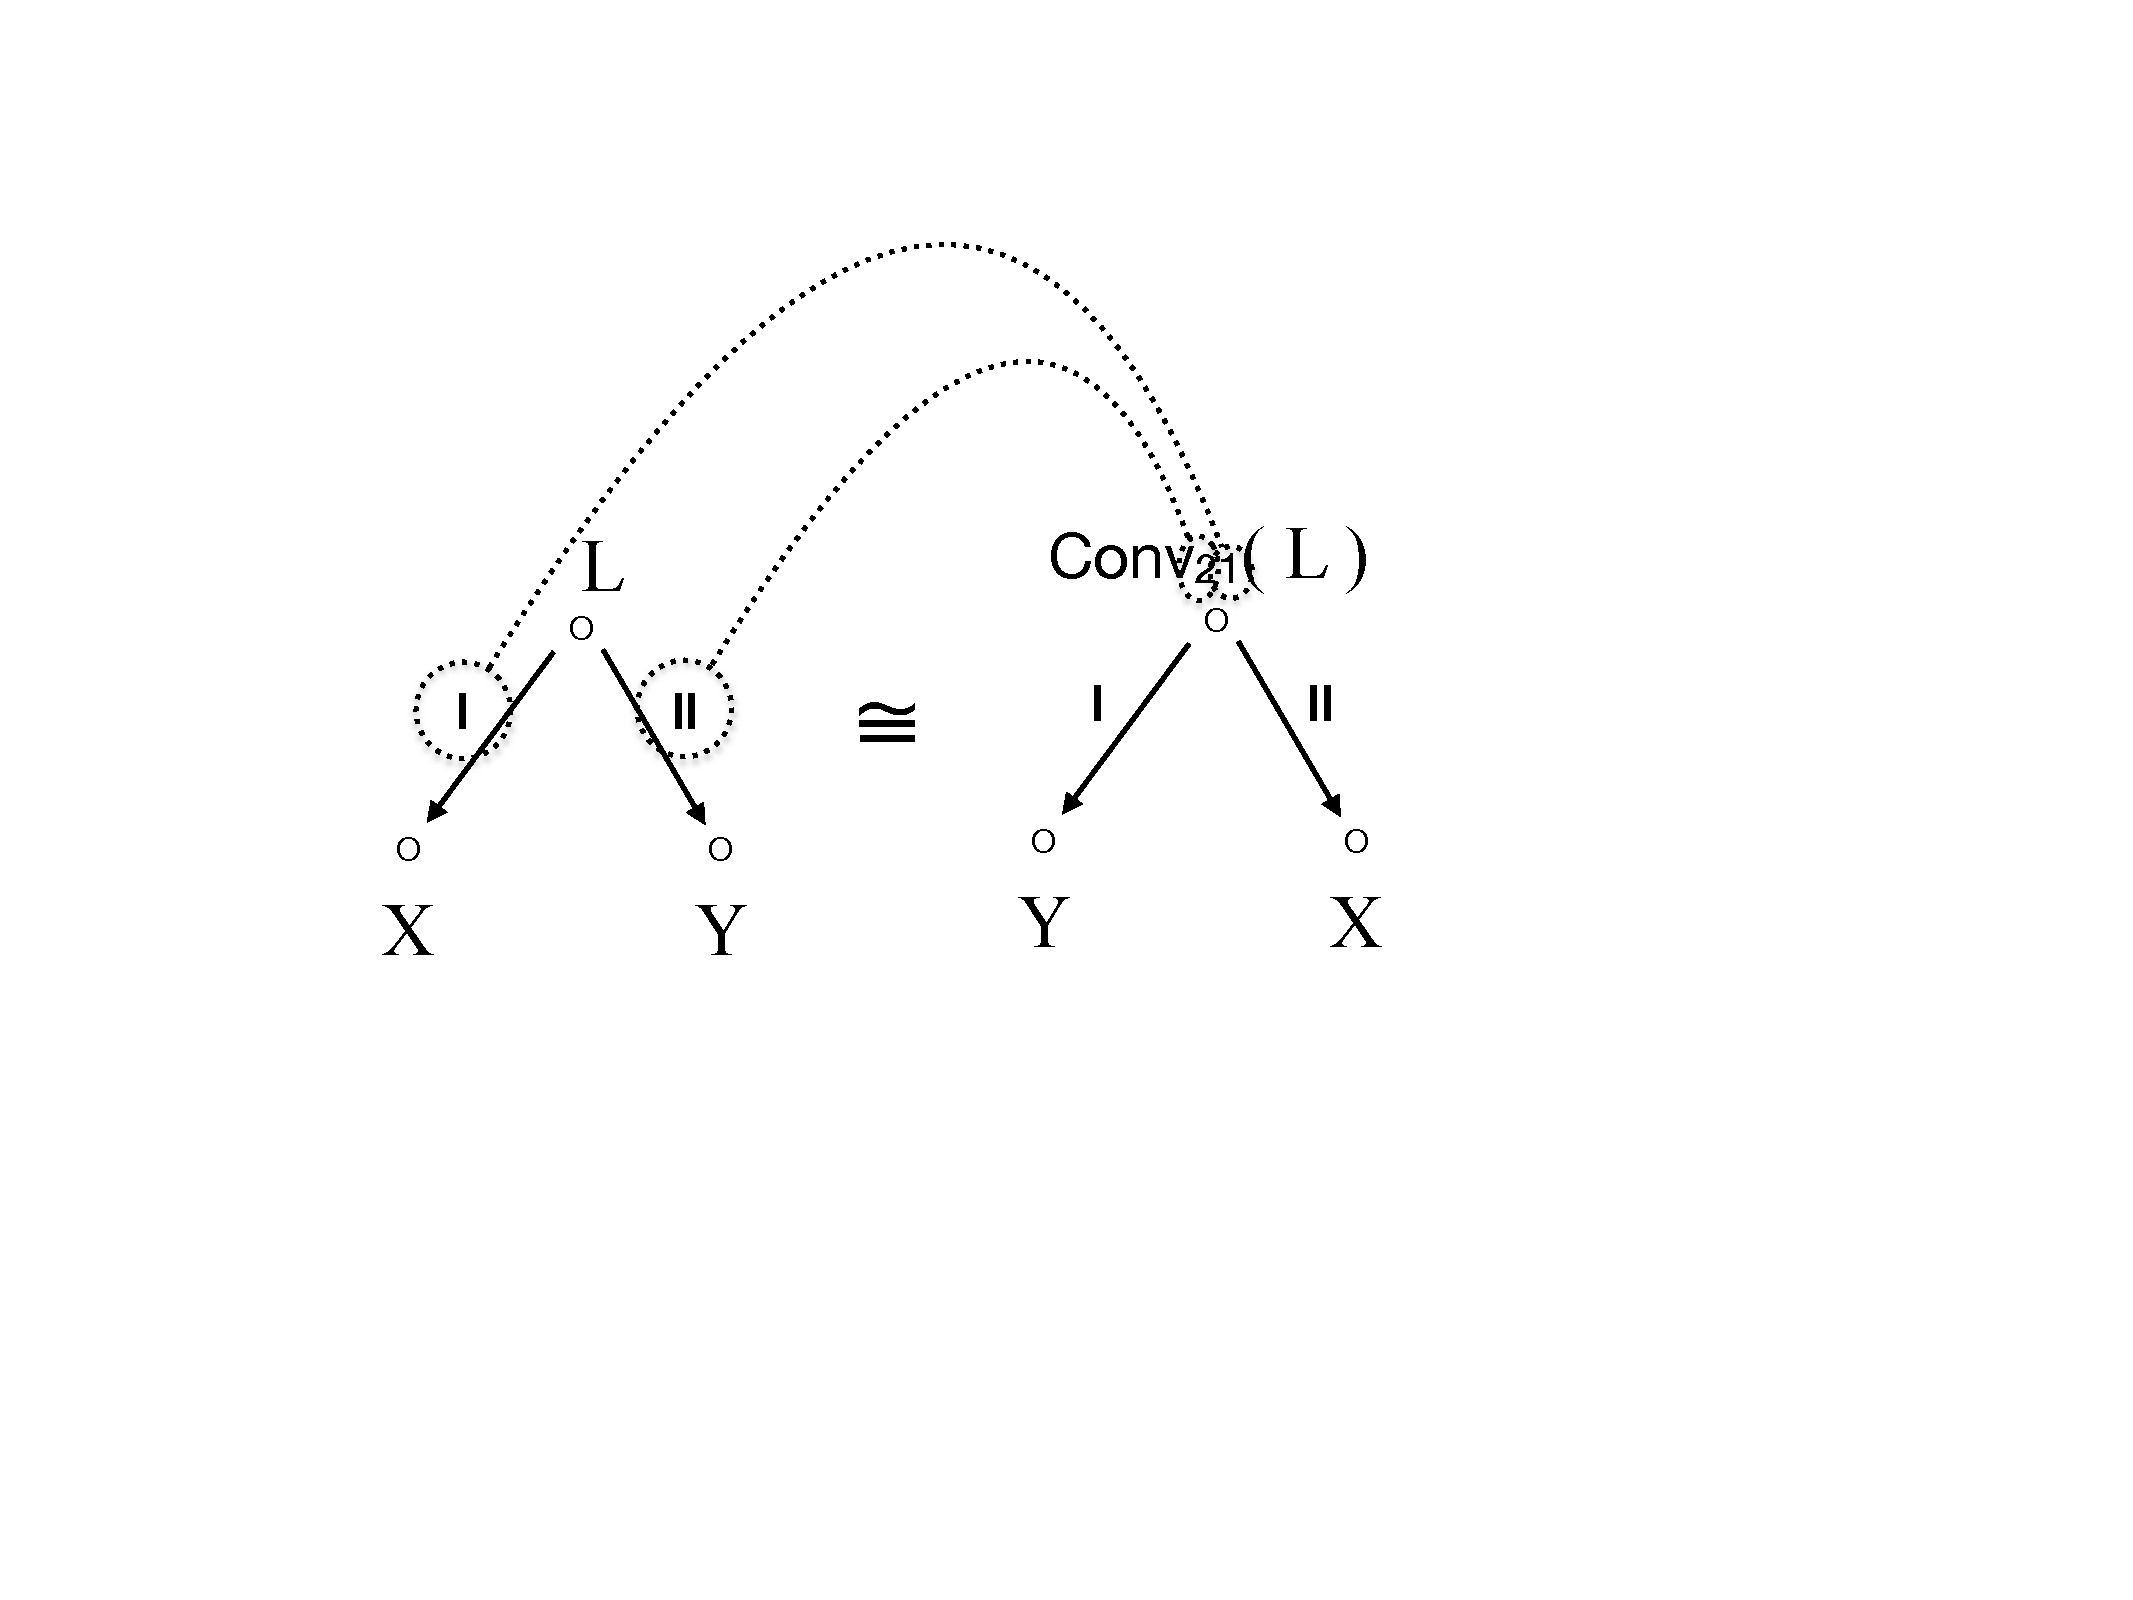
\includegraphics[width=5.5cm]{Fig/ParaLF/CorrSyntPConv-21.pdf}\\
{\small For instance: \textit{X follows Y.}\enskip$\cong$\enskip\textit{Y precedes}\tsub{\lfappl{Conv$_{21}$}{\textit{follow}}} \textit{X.}}
\caption{Correspondence between L's DSyntAs and those of \lfappl{Conv\tsub{21}}{L}}\label{fig:Conv-ijk}
\end{figure}

\begin{longtable*}[l]{ l l >{\raggedright\arraybackslash}p{6.5cm} }

\multicolumn{3}{l}{\textbf{French}} \\

\lfappl{Conv\tsub{21}}{\textit{inclure} \lfgp{X is a set}} & = & \textit{appartenir}\textbf{,} \idiom{\textit{faire partie}} \\
\lfappl{Conv\tsub{3214}}{\textit{prêter}} & = & \textit{emprunter} \\
\multicolumn{3}{l}{\quad\lfgp{N\tsub{X} \textit{prête} N\tsub{Y} \textit{à} N\tsub{Z} \textit{pour la période} N\tsub{W}}} \\
\lfappl{Conv\tsub{3214$\cap$}}{\textit{acheter}} & = & \textit{vendre} \\
\multicolumn{3}{l}{\quad\lfgp{N\tsub{X} \textit{achète} N\tsub{Y} \textit{à} N\tsub{Z} \textit{pour} N\tsub{W}}} \\
\lfappl{Conv\tsub{3214$\cap$}}{\textit{vendre}} & = & \textit{acheter} \\
\lfappl{Conv\tsub{1432$\supset$}}{\textit{acheter}} & = & \textit{payer} \\
\lfappl{Conv\tsub{21}}{\lfgp{\textit{être}} \textit{parent}} & = & \lfgp{\textit{être}} \textit{enfant} \\
\lfappl{Conv\tsub{213}}{\lfgp{\textit{être}} \textit{maître}} & = & \lfgp{\textit{être}} \textit{élève} \lfgp{\textit{du prof. Ménard en math}} \\
\vspace{2pt}\lfappl{Conv\tsub{21}}{\textit{meilleur}} & = & \textit{pire}\vspace{6pt} \\

\multicolumn{3}{l}{\textbf{Russian}} \\

\lfappl{Conv\tsub{21}}{\textit{soder\v{z}at\palati} \lfgp{X is a set}} & = & \textit{prinadle\v{z}at\palati} \\
\lfappl{Conv\tsub{3214}}{\textit{odol\v{z}it\palati}\sensenum{I} \lfgp{N\tsub{\textsc{dat}}}} & = & \textit{odol\v{z}it\palati}\sensenum{II} \lfgp{\textit{u} N\tsub{\textsc{gen}}} \\
\multicolumn{3}{l}{\quad\lfgp{N\tsub{X-\textsc{nom}} \textit{odol\v{z}il} N\tsub{Y-\textsc{acc}} N\tsub{Z-\textsc{dat}} \textit{na vremja} N\tsub{W-\textsc{acc}}}} \\
\lfappl{Conv\tsub{3214$\cap$}}{\textit{kupit\palati}} & = & \textit{prodat\palati} \\
\multicolumn{3}{l}{\quad\lfgp{N\tsub{X-\textsc{nom}} \textit{kupil} N\tsub{Y-\textsc{acc}} \textit{u} N\tsub{Z-\textsc{gen}} \textit{za} N\tsub{W-\textsc{acc}}}} \\
\lfappl{Conv\tsub{3214$\cap$}}{\textit{prodat\palati}} & = & \textit{kupit\palati} \\
\lfappl{Conv\tsub{1432$\supset$}}{\textit{kupit\palati}} & = & \textit{zaplatit\palati} \\
\lfappl{Conv\tsub{21}}{\lfgp{\textit{byt\palati}} \textit{roditelem}} & = & \lfgp{\textit{byt\palati}} \textit{rebënkom} \\
\lfappl{Conv\tsub{213}}{\lfgp{\textit{byt\palati}} \textit{u\v{c}itelem}} & = &\lfgp{\textit{byt\palati}} \textit{u\v{c}enikom} \lfgp{\textit{prof. Menara po matematike}} \\
\lfappl{Conv\tsub{21}}{\textit{tja\v{z}elee}} & = & \textit{leg\v{c}e} \\

\end{longtable*}

\refstepcounter{LFlist}
\subsubsection*{{\small [\arabic{LFlist}]} \lf{Anti} \lfgp{{\scriptsize Latin} *\textit{antonymum}}: antonym}\label{lf:Anti}
\addcontentsline{toc}{subsection}{{\footnotesize [\arabic{LFlist}]} \lf{Anti}: antonym}\index[lf]{Anti@\lf{Anti}|emph}\index[notion]{antonym|emph}

\lfappl{Anti}{L} has a meaning opposite to that of L and is, therefore, a possible substitute for L in the syntactic structure of the utterance with preservation of the meaning, but under the condition that a negation is added to \lfappl{Anti}{L} as illustrated in \Next[a--b].

\begingroup

\ex. \a. Chris was \emph{absent} from the meeting.\\*
         $\equiv$
     \b. Chris was \emph{not present}\tsub{\lfappl{Anti}{\textit{absent}}} at the meeting.

\endgroup

However, such equivalence is valid only for contradictory antonyms\index[notion]{antonym!contradictory [=~complementary] \tld} (see type~\ref{txt:contradictoryAntonym} of antonyms after the illustrations below); with other types of antonyms, the semantic equivalence is only approximate or does not obtain at all. The paraphrastic\index[notion]{paraphrase} relation holding between a lexical unit L and \lfappl{Anti}{L}\thinspace+\thinspace{}Negation is too complex to be summarized here with a single paraphrasing rule, and it is considered below separately for each of the four types of antonyms.

\begin{longtable*}[l]{ l l >{\raggedright\arraybackslash}p{7cm} }

\multicolumn{3}{l}{\textbf{English}} \\*

\lfappl{Anti}{\textit{respect}\tsub{(N)}} & = & \textit{disrespect}\tsub{(N)} \\
\lfappl{Anti}{\textit{small}\tsub{(Adj)}} & = & \textit{big}\tsub{(Adj)} \\
\lfappl{Anti}{\textit{hot}} & = & \textit{cold}\tsub{(Adj)} \\
\lfappl{Anti}{\textit{with}} & = & \textit{without} \\
\lfappl{Anti}{\textit{dress}\tsub{(V)}} & = & \textit{undress}\tsub{(V)} \\
\lfappl{Anti\tsub{$\cap$}}{\textit{build}\tsub{(V)}} & = & \textit{destroy} \\
\vspace{2pt}\lfappl{Anti}{\textit{Yummy!}} & = & \textit{Yuck!} \\[6pt]

\multicolumn{3}{l}{\textbf{French}} \\*

\lfappl{Anti}{\textit{respect}} & = & \textit{irrespect} \\
\lfappl{Anti\tsub{$\supset$}}{\textit{mentionner}} & = & \idiom{\textit{passer sous silence}} \\
\lfappl{Anti}{\textit{petit}\tsub{(Adj)}} & = & \textit{grand}\tsub{(Adj)} \\
\lfappl{Anti}{\textit{chaud}\tsub{(Adj)}} & = & \textit{froid}\tsub{(Adj)} \\
\lfappl{Anti}{\textit{avec}} & = & \textit{sans} \\
\lfappl{Anti}{\textit{habiller}} & = & \textit{déshabiller} \\
\lfappl{Anti\tsub{$\cap$}}{\textit{construire}} & = & \textit{détruire} \\*
\vspace{2pt}\lfappl{Anti}{\textit{Miam !}} & = & \textit{Beurk !}\vspace{6pt} \\

\multicolumn{3}{l}{\textbf{Russian}} \\*

\lfappl{Anti}{\textit{uva\v{z}enie}} & = & \textit{neuva\v{z}enie} \\
\lfappl{Anti\tsub{$\supset$}}{\textit{upomjanut\palati}} & = & \idiom{\textit{obojti mol\v{c}aniem}} \\
\lfappl{Anti}{\textit{malen\palati{}kij}} & = & \textit{bol\palati{}\v{s}oj} \\
\lfappl{Anti}{\textit{gorja\v{c}ij}} & = & \textit{xolodnyj} \\
\lfappl{Anti}{\textit{s}} & = & \textit{bez} \\
\lfappl{Anti}{\textit{odet\palati}} & = & \textit{razdet\palati} \\
\lfappl{Anti\tsub{$\cap$}}{\textit{stroit\palati}} & = & \textit{razru\v{s}at\palati} \\
\lfappl{Anti}{\textit{Ux\onewdf{}ty!}}\footnotemark\index[notion]{wordform} & = & \textit{Fu!} \\

\end{longtable*}\footnotetext{\label{fn:greyUnderscoring}The grey underscoring of the space between two strings of letters, as in \textsc{ux\onewdf{}ty}, shows that, linguistically speaking, this expression is a single wordform, which is traditionally spelled in two words (cf. \textsc{at\onewdf{}all}, \textsc{at\onewdf{}last} or \textsc{by\onewdf{}far}).}

Antonyms come in four types: contradictory, contrary, scalar and positioning antonyms.

\begin{enumerate}

\item \notion{Contradictory} (or~\notion{complementary}) \notion{antonyms}\index[notion]{antonym!contradictory [=~complementary] \tld}\phantomsection\label{txt:contradictoryAntonym}. A contradictory antonym is opposed to its ``partner'' by a negation of the highest level of its meaning, i.e., that applies to the central component of its lexicographic definition\index[notion]{component of a definition!central \tld}\index[notion]{definition!central component of a \tld} \parencite[Sec.~2.4.1]{MelcukPolguere2018}: `\lfappl{Anti}{L}' $=$ `non L'. Two mutually contradictory antonyms represent the two values of a binary category. For instance, \textsc{present}\tsub{(Adj)} \senseex{in a room} is a contradictory antonym of \textsc{absent}\tsub{(Adj)} \senseex{from a room}:

\begin{tabular}{ l l p{7cm} }

`[X] absent from Y' & = & `[X] \emph{not} present in Y' \\

\end{tabular}

Contradictory antonyms do not (or hardly) allow for gradation: *\textit{more}\verythinspace/\verythinspace\textit{less present in a room}. In contrast, the remaining three types of antonyms are gradable.

\item \notion{Contrary antonyms}\index[notion]{antonym!contrary \tld}. Two mutually contrary antonyms are opposed by a negation that is deeply embedded in the lexicographic definition\index[notion]{definition!lexicographic \tld} of one of them, i.e., that applies to a peripheral component\index[notion]{component of a definition!peripheral \tld}\index[notion]{definition!peripheral component of a \tld}. For instance, \textsc{close}\tsub{(V)} \senseex{a door} is a contrary antonym of \textsc{open}\tsub{(V)} \senseex{a door}:

\begin{tabular}{ l l p{7cm} }

`X opens Y' & = & `X causes that Y becomes open\tsub{(Adj)}' \\
`X closes Y' & = & `X causes that Y becomes \emph{not} open\tsub{(Adj)}' \\

\end{tabular}

These semantic decompositions show that `close\tsub{(V)}' $\neq$ `not open\tsub{(V)}' and, therefore, that \textsc{close}\tsub{(V)} and \textsc{open}\tsub{(V)} are not contradictory antonyms.

\item\phantomsection\label{item:scalarAntonym} \notion{Scalar antonyms}\index[notion]{antonym!scalar \tld}. They are opposed by the components `more' $\sim$ `less' in their lexicographic definitions\index[notion]{definition!lexicographic \tld}: `more'\slashs`less' indicates the position on a gradable scale, or on an axis. For instance, \textsc{heavy}\tsub{(Adj)} and \textsc{light}\tsub{(Adj)} are scalar antonyms:

\begin{tabular}{ l l p{7.5cm} }

`X is heavy' & = & `X's weight is \emph{higher} [=~`\emph{more} high'] than the normal weight of Xs' \\
`X is light' & = & `X's weight is \emph{lower} [=~`\emph{less} high'] than the normal weight of Xs' \\

\end{tabular}

The opposition between `more' and `less' is reducible to the opposition by negation \parencite[190]{Melcuk2015a-e}. Note that if two adjectives are scalar antonyms, their comparative degrees are conversives as well; thus, we have `X is heavier than Y' = `Y is lighter than~X'.

\item \notion{Positioning antonyms}\index[notion]{antonym!positioning \tld}. These antonyms denote two opposite spatial or temporal positions (in a literal or metaphorical sense). For instance, \textsc{top}\tsub{(N)} \senseex{the top of the shelves} and \textsc{bottom}\tsub{(N)} \senseex{the bottom of the shelves} are positioning antonyms:

\begin{tabular}{ l l p{7.2cm} }
`top of X' & = & `part of X that is the \emph{furthest} [=~`\emph{least} close'] to the surface on which X is located' \\
`bottom of X' & = & `part of X that is the \emph{closest} [=~`\emph{most} close'] to the surface on which X is located' \\
\end{tabular}

\end{enumerate}

As is seen, all types of antonyms are based on negation. It is the position of negation in the lexicographic definition\index[notion]{definition!lexicographic \tld} of lexical units that are \lfappl{Anti}{L} that determines the type of antonymy. In the enumeration of the four antonym types above, we started with the negation occupying the uppermost position in the definition and concluded with the negation that is the most deeply embedded.

A lexical unit can have antonyms of different types. Such is, for instance, the lexeme \textsc{destroy}, appearing in \Next: 

\begingroup
\small

\ex. They destroyed the bridge. \\
     `They caused that the bridge ceased to exist' = `They caused the bridge to \emph{not}[exist]'

\endgroup

\textsc{destroy} has two antonyms: a contradictory one -- \textsc{spare}\tsub{(V)}, cf. \Next, and a contrary one -- \textsc{build}\tsub{(V)}, cf. \NNext.

\begingroup
\small

\ex. They spared the bridge. \\
         `They \emph{not}[caused that the bridge ceased to exist]'
         
\ex. They built the bridge. \\
         `They caused that the bridge \emph{not}[\emph{not}[exist]]' = `They caused that the bridge exists' \\
         \hphantom{......................................................................................}(`\emph{not}[\emph{not}[exist]]' = `exist')

\endgroup

For all four types of antonyms only one LF is used: \lf{Anti}. Theoretically speaking, it is easy to distinguish the four \lf{Anti} LFs by means of super- or subscripts -- e.g. \lf{Anti\tsup{contrad}}, \lf{Anti\tsup{contrary}}, etc. This is, however, superfluous, since each antonym should have its own lexicographic description -- in particular, its definition -- in a lexicographic model\index[notion]{lexicon!\tld\ model}\index[notion]{model!lexicon \tld}\index[notion]{lexicography}, which allows the user of the model to see the meaning relation\index[notion]{meaning!\tld\ relation}\index[notion]{relation!meaning \tld} between L and \lfappl{Anti}{L}.

Note that the cases where a lexical unit has antonyms of different types are infrequent enough.

\largerpage
Sometimes the negation underlying the antonymy has to be encoded  as such in LF formulas; then the LF \lf{Non}\index[lf]{Non@\lf{Non}|emph} `not' is used. Thus, \lf{Non} -- rather than \lf{Anti} -- combines with semantically empty LFs, such as those that represent support verbs\index[notion]{support verb}\index[notion]{verb!support \tld} (\lf{Oper\tsub{i}}\index[lf]{Operi@\lf{Oper\tsub{i}}}, \lf{Func\tsub{i}}\index[lf]{Funci@\lf{Func\tsub{i}}} and \lf{Labor\tsub{ij}}\index[lf]{Laborij@\lf{Labor\tsub{ij}}}, in \chapref{chap:syntLFs}, \sectref{sec:verbeSupport}). And, from a logical viewpoint, a semantically empty verb cannot have an antonym: an antonym of L is supposed to have an opposite meaning with respect to that of L, while a light verb has no meaning. Therefore, we have:

\begingroup
\small
\ex. \begingroup\setlength{\tabcolsep}{2pt}
\begin{tabular}[t]{ l l >{\raggedright\arraybackslash}p{8cm} }
\lfappl{Oper\tsub{1}}{\textit{consent}\tsub{(N)}} & = & \textit{give}\textbf{,} \textit{grant} \lfgp{\textsc{art} \tld} \\
\lfappl{NonOper\tsub{1}}{\textit{consent}\tsub{(N)}} & = & \textit{refuse} \lfgp{\textsc{art} \tld} \\
\end{tabular}\endgroup

\endgroup

\begin{historicalremark}
The previous presentations of LFs, e.g. \textcite[75--81]{MelcukEtAl1999}, did not introduce the LF \lf{Non} explicitly. In these publications the LF \lf{Non} (as \lf{Non} or \lf{non}) was simply smuggled into complex LF formulas.
\end{historicalremark}

\section{Three LFs related to \lf{Syn} and \lf{Anti}: \lf{Gener}, \lf{Figur}, \lf{Contr}}\label{sec:LFapparenteesSynAnti}

\refstepcounter{LFlist}
\subsubsection*{{\small [\arabic{LFlist}]} \lf{Gener} \lfgp{{\scriptsize Latin} \textit{genus}}: generic term}\label{lf:Gener}
\addcontentsline{toc}{subsection}{{\footnotesize [\arabic{LFlist}]} \lf{Gener}: generic term}\index[lf]{Gener@\lf{Gener}|emph}

\lfappl{Gener}{L} -- a generic term\index[notion]{generic term|emph} for L -- stands for the name of one of the semantic classes\index[notion]{semantic!\tld\ class} to which L's meaning may belong. It applies to L of any PoS and, like \lf{Syn}, it borrows L's PoS:

\begin{quote}
\begingroup
\small
\phantomsection\label{txt:PoSGener}\begin{tabular}{ l c c c c c }
   \midrule
   \multicolumn{6}{l}{\lf{Gener}: borrows L's PoS} \\
   \midrule
   \textbf{L} & V & N & Adj & Adv & Claus \\
   \midrule
   \textbf{\lfappl{Gener}{L}} & V & N & Adj & Adv & Claus\lfgp{?} \\
   \midrule
\end{tabular}
\endgroup
\end{quote}

\index[notion]{government pattern!\tld\ of an LF value element}\index[notion]{value of an LF!government pattern of an element of the \tld}
\begin{longtable*}[l]{ l l >{\raggedright\arraybackslash}p{8cm} }

\multicolumn{3}{l}{\textbf{English}} \\*

\lfappl{Gener}{\textit{love}\tsub{(N)}} & = & \textit{feeling} \lfgp{\textit{of} \tld}\textbf{;} \textit{emotion} \lfgp{\textit{of} \tld} \\%[1pt]
\lfappl{Gener}{\textit{gas}\tsub{(N)}} & = & \lfgp{\textit{gaseous}} \textit{substance} \\
\vspace{2pt}\lfappl{Gener}{\textit{see}\tsub{(V)}} & = & \textit{perceive} \lfgp{\textit{visually}} \\[6pt]

\multicolumn{3}{l}{\textbf{French}} \\*

\lfappl{Gener}{\textit{amour}} & = & \textit{sentiment} \lfgp{\textit{d'}\tld}\textbf{;} \textit{émotion}  \\
\lfappl{Gener}{\textit{gaz}} & = & \textit{substance} \lfgp{\textit{gazeuse}}\\
\vspace{2pt}\lfappl{Gener}{\textit{voir}} & = & \textit{percevoir} \lfgp{\textit{visuellement}} \\[6pt]

\multicolumn{3}{l}{\textbf{Russian}} \\*

\lfappl{Gener}{\textit{ljub\suffixsplit{}ov\palati}} & = & \textit{\v{c}uvstvo} \lfgp{\tld\textit{vi}}\textbf{;} \textit{èmocija} \\
\lfappl{Gener}{\textit{gaz}} & = & \lfgp{\textit{gazoobraznoe}} \textit{ve\v{s}\v{c}estvo} \\
\lfappl{Gener}{\textit{videt\palati}} & = & \textit{vosprinimat\palati} \lfgp{\textit{zritel\palati{}no}} \\

\end{longtable*}

\paragraph*{Identifying \lfappl{Gener}{L}.}

For a lexical unit to belong to the value of \lfappl{Gener}{L} it is necessary and sufficient to appear in the following constructions:

\begin{itemize}

\item for nouns: L\textit{,} L′\textit{,} L′′\textit{, ... and other} \lfappl{Gener}{L} 

\begingroup
\small

\ex. \textit{melons, raspberries, mangoes, ... and other fruits}\tsub{\lfappl{Gener}{\textit{melon}}}

\endgroup

\item for verbs, adjectives and adverbs: L\textit{,} L′\textit{,} L′′\textit{, ... and} \lfappl{Gener}{L} \textit{in other ways}

\begingroup
\small

\ex. \a. \textit{see, smell, ... and perceive}\tsub{\lfappl{Gener}{\textit{see}}} \textit{in other ways}
     \b. \textit{fried, boiled, ... and cooked}\tsub{\lfappl{Gener}{\textit{fried}}} \textit{in other ways}

\endgroup

\end{itemize}

These examples show that \lf{Gener} is a powerful classifier: it identifies numerically important semantic classes\index[notion]{semantic!\tld\ class} of lexical units. For instance:

\begin{itemize}

\item the noun \textsc{dog} is \lf{Gener} of \textsc{basset}, \textsc{bulldog}, \textsc{collie}, \textsc{dachshund}, \textsc{dalmatian}, \idiom{\textsc{german shepherd}}, \textsc{husky}, \textsc{labrador}, \textsc{poodle}, \textsc{setter},~...
    
\item the noun \textsc{feeling}\index[notion]{noun!\tld\ of feeling} is \lf{Gener} of \textsc{adoration}, \textsc{despair}\tsub{(N)}, \textsc{dread}\tsub{(N)}, \textsc{excitement}, \textsc{fear}\tsub{(N)}, \textsc{gratitude}, \textsc{love}\tsub{(N)}, \textsc{remorse}, ...

\end{itemize}

The compatibility of a \lf{Gener} with the above constructions allows for the distinction between \lf{Gener} and \lf{Syn}\tsub{$\subset$}\index[lf]{Syn@\lf{Syn}!\lf{Syn}\tsub{$\subset$}}. Thus, \textsc{dream}\tsub{(N)} is a \lf{Syn}\tsub{$\subset$} of \textsc{nightmare}, rather than a \lf{Gener}, because English does not have an important enough class of lexical units denoting different types of dreams.

\paragraph*{\lf{Gener}-based paraphrasing.}\label{par:GenerBasedParaphrasing}\index[notion]{paraphrase}

The lexical stock and the lexical cooccurrence\index[notion]{cooccurrence, restricted!lexical \tld} of the language allowing, a given \lfappl{Gener}{L} can be used in the two following equivalences grouped under paraphrasing rule \textbf{R\tsub{\lf{Gener}}}:\footnote{These equivalences are described by two distinct paraphrasing rules (Rules~4 and~5) in \textcite[p.\thinspace152]{Melcuk2013c-e}.}

\begin{center}
\phantomsection\label{txt:RParaphGener}\APolbox{11.2cm}{%
\begin{tabular}{ l l l }
\textbf{R\tsub{\lf{Gener}}:} & a) & L\tsub{(N)}\enskip{\small$\equiv$}\enskip\lfappl{Gener}{L\tsub{(N)}}\thinspace\syntRel{R}\thinspace L\tsub{(N)} \vspace{3pt}\\

&
& \begingroup\setlength{\tabcolsep}{0pt}\renewcommand{\arraystretch}{.8}\begin{tabular}{ l }
{\small\textit{anger}\tsub{(N)}\enskip$\equiv$\enskip\textit{feeling}\tsub{\lfappl{Gener}{\textit{anger}$_\text{(N)}$}} \textit{of anger}} \\
{\small\textit{submission}\enskip$\equiv$\enskip\textit{attitude}\tsub{\lfappl{Gener}{\textit{submission}}} \textit{of submission}} \\
{\small\textit{smell}\tsub{(N)}\enskip$\equiv$\enskip\textit{sense}\tsub{\lfappl{Gener}{\textit{smell}$_\text{(N)}$}} \textit{of smell}}
\end{tabular}\endgroup  \vspace{3pt}\\

& b) & L\enskip{\small$\equiv$}\enskip\lfappl{Gener}{L}\thinspace\syntRel{R}\thinspace\lfappl{A\tsub{0}/Adv\tsub{0}/Adv\tsub{1}}{L}  \vspace{3pt}\\

&
& \begingroup\setlength{\tabcolsep}{0pt}\renewcommand{\arraystretch}{.8}\begin{tabular}{ l  }
{\small For L\tsub{(N)}: \textit{anger}\tsub{(N)}\enskip$\equiv$\enskip\textit{angry}\tsub{\lfappl{A\tsub{0}}{\textit{anger}$_\text{(N)}$}} \textit{feeling}\tsub{\lfappl{Gener}{\textit{anger}$_\text{(N)}$}}} \\
{\small For L\tsub{(V)}: \textit{see}\enskip$\equiv$\enskip\textit{perceive}\tsub{\lfappl{Gener}{\textit{see}}} \textit{visually}\tsub{\lfappl{Adv\tsub{1}}{\textit{see}}}} \\
{\small For L\tsub{(Adj)}: \textit{visual}\enskip$\equiv$\enskip\textit{visually}\tsub{\lfappl{Adv\tsub{0}}{\textit{visual}}} \textit{perceptible}\tsub{\lfappl{Gener}{\textit{visual}}}} \\
\end{tabular}\endgroup  \vspace{3pt}\\
\multicolumn{3}{>{\raggedright\arraybackslash}p{10cm}}{{\small See below for the description of the LFs \lf{A\tsub{0}} (\sectref{sec:derivationsStructurales}, [\ref{lf:A0}], p.\thinspace\pageref{lf:A0}), \lf{Adv\tsub{0}} (\sectref{sec:derivationsStructurales}, [\ref{lf:Adv0}], p.\thinspace\pageref{lf:A0}) and \lf{Adv\tsub{1}} (\sectref{sec:derivAdvAct}, [\ref{lf:Adv-i}], p.\thinspace\pageref{lf:Adv-i}).}} \\
\end{tabular}
}
\end{center}\index[notion]{paraphrase!deep-syntactic paraphrasing rule!\textbf{R\tsub{\lf{Gener}}}|emph}\index[lf]{A0@\lf{A\tsub{0}}}\index[lf]{Adv0@\lf{Adv\tsub{0}}}\index[lf]{Advi@\lf{Adv\tsub{i}}!\lf{Adv\tsub{1}}}\index[notion]{relation!deep-syntactic \tld}\index[notion]{actantial relation}\index[notion]{relation!actantial \tld}

In subrules a) and b) above, the deep-syntactic relation~\syntDname{R} on the right-hand side of the equivalence remains unspecified, as it varies according to the semantic valence\index[notion]{valence!semantic \tld} and government pattern\index[notion]{government pattern} of each particular \lfappl{Gener}{L}; for instance:

\begingroup
\small

\ex. \a. \textsc{color}\tsub{(N, `color of X that is Y')}: \textit{the color}\tsub{\lfappl{Gener}{\textit{purple}\tsub{(N)}}}\thinspace\syntRel{II}\thinspace\textit{purple}
     \b. \textsc{feeling}\tsub{(`feeling of X towards Y that is Z')}: \textit{the feeling}\tsub{\lfappl{Gener}{\textit{love}\tsub{(N)}}}\thinspace\syntRel{III}\thinspace\lfgp{\textit{of}} \textit{love}
     \c. \textsc{number}\tsub{(N)}: \textit{the number}\tsub{\lfappl{Gener}{\textit{nine}}}\thinspace\syntRel{ATTR}\thinspace\textit{nine}

\endgroup

\paragraph*{Multiplicity of the values of \lfappl{Gener}{L}.}

A lexical unit L can have multiple elements of the value for \lfappl{Gener}{L}. This happens in two cases.

The first case is trivial. As for any other LF, there can be multiple elements of the value of \lfappl{Gener}{L} that are (quasi-)synonyms; for instance:

\begingroup
\small

\ex. \begingroup\setlength{\tabcolsep}{2pt}
\begin{tabular}[t]{ l l >{\raggedright\arraybackslash}p{8cm} }
\lfappl{Gener}{\textit{fear}\tsub{(N)}} & = & \textit{feeling} \lfgp{\textit{of} \tld}\textbf{;} \textit{emotion} \lfgp{\textit{of} \tld} \\*
& & \lfgp{\lfappl{Syn\tsub{$\supset$}}{\textit{feeling}} = \textit{emotion}} \\*
\lfappl{Gener}{\textit{bin}\tsub{(N)}} & = & \textit{container}\textbf{;} \textit{receptacle} \\*
& & \lfgp{\lfappl{Syn\tsub{$\cap$}}{\textit{container}} = \textit{receptacle}} \\\end{tabular}\endgroup

\endgroup

The second case is more remarkable as it is conditioned by the special character of L's meaning. Two subcases are distinguished:

\begin{itemize}

\item L denotes\index[notion]{denotation} more than one kind of thing and, therefore, L belongs to more than one semantic class\index[notion]{semantic!\tld class}. This phenomenon  corresponds to L's \notion{semantic ambivalence}\index[notion]{ambivalence, semantic}\index[notion]{semantic!\tld\ ambivalence} \parencite{MilicevicPolguere2010-e,SmirnovaTolochin2018}, that is, to the presence of a disjunction in L's definition.\footnote{See also the related notions of \emph{facet}\verythinspace/\verythinspace\emph{subsense} \parencite{Cruse1995} and \emph{logical polysemy} \parencite{Pustejovsky1995}.}

\item  L's definition contains a classifying component -- called \notion{semantic-class marking component}\index[notion]{component of a definition!semantic-class marking \tld} \parencite[Sec.~2.4.1.2]{MelcukPolguere2018} -- that underlies a value of \lfappl{Gener}{L}.   If, at the same time, the central component\index[notion]{definition!central component of a \tld}\index[notion]{component of a definition!central \tld} of L's definition\index[notion]{definition!lexicographic \tld} underlies also a value of \lfappl{Gener}{L}, which is a prototypical case, L obtains more than one type of \lfappl{Gener}{L}.

\end{itemize}

Let us take an example: the definition of the lexeme \textsc{snow}\tsub{(N)}, which illustrates both situations.

\begingroup
\small

\ex. \label{ldef:defSNOW-n}\APolbox{11cm}{%
   \begin{tabular}{ l p{8cm} }
   \textit{snow on Y} :
   &
   frozen water that is falling or has fallen from the sky on geographical place Y \newline
   \setlength{\tabcolsep}{.5pt}\begin{tabular}{ p{0.2cm} >{\raggedright\arraybackslash}p{6cm} }
   \SpecDiff & in the form of white flakes \\
   \end{tabular} \\
   & or \\
   &
   this falling \newline
   \setlength{\tabcolsep}{.5pt}\begin{tabular}{ p{0.2cm} >{\raggedright\arraybackslash}p{6cm} }
   \SpecDiff & which is a weather phenomenon \\
   \end{tabular} \\
%   \multicolumn{2}{|l|}{Ex.: \textit{How is an atom of the \textbf{element} 54 (Xe) likely to act during a chemical reaction?}} \\
\end{tabular}
}

\endgroup

In the above definition, the disjunction in the central component (`or') and the semantic-class marking component (`which is a weather phenomenon') combine to produce two types of \lfappl{Gener}{\textit{snow}\tsub{(N)}}:

\begingroup
\small

\ex. \begingroup\setlength{\tabcolsep}{2pt}
\begin{tabular}[t]{ l l >{\raggedright\arraybackslash}p{7cm} }
\lfappl{Gener}{\textit{snow}\tsub{(N)}} & = & (i)\hspace{3pt} \textit{substance}\textbf{;} \\*
& & (ii) \textit{precipitation}\textbf{,} \idiom{\textit{weather condition}} \\
\end{tabular}\endgroup

\endgroup

Formula \Last presupposes that we are dealing with one single sense of \textsc{snow}\tsub{(N)}, that is, with one lexeme, and not with a case of polysemy\index[notion]{polysemy}, that is, with two lexemes -- one denoting\index[notion]{denotation} a substance and one denoting the event of its falling. This can be demonstrated using the \emph{Unifying cooccurrence}\index[notion]{cooccurrence, restricted} criterion presented in \textcite[Ch.~11, Sec.~3.2.2]{Melcuk2013c-e}. Indeed, a given occurrence of \textit{snow}\tsub{(N)} in an utterance can be used to refer to both substance and event simultaneously:

\begingroup
\small

\ex. The snow that \emph{started} \lfgp{snow as precipitation} this morning \\
     \hphantom{.....}is beautifully \emph{fluffy} \lfgp{snow as substance}.

\endgroup

For this reason, both types of denotation of \textsc{snow}\tsub{(N)} (substance and meteorological event) have to be considered as belonging to one lexical unit, with a disjunctive central component\index[notion]{definition!lexicographic \tld}\index[notion]{definition!disjunctive central component of a \tld}\index[notion]{component of a definition!disjunctive central \tld} in its definition.

 The classifying power of \lf{Gener} makes this LF particularly important in the structuring of natural language lexical networks\index[notion]{lexical network}\index[notion]{network \lfgp{see also \textit{graph}}!lexical \tld} and in the description of lexical regularities\index[notion]{regularity} -- see \chapref{chap:NotionLF}, \sectref{sec:generalizationsGener}.
 
\begin{furtherreading}
For more on generic terms and lexicographic definitions, see \textcite[Sec.~3]{Polguere2022a} and \textcite{Goddard2017}.
\end{furtherreading}

\refstepcounter{LFlist}
\subsubsection*{{\small [\arabic{LFlist}]} \lf{Figur} \lfgp{{\scriptsize Latin} \textit{figuraliter} `figuratively'}: figurative term}\label{lf:Figur}
\addcontentsline{toc}{subsection}{{\footnotesize [\arabic{LFlist}]} \lf{Figur}: figurative term}\index[lf]{Figur@\lf{Figur}|emph}

\lfappl{Figur}{L} is a metaphorical expression having the same meaning as the noun L plus a somehow artistic representation of L; it is either a lexical unit or a collocation whose base is L and the collocate, a noun that takes L as its DSyntA\thinspace\syntDname{I}. The relation of paraphrase between L and \lfappl{Figur}{L} is accounted for by the \textbf{R\tsub{\lf{Figur}}}\index[notion]{paraphrase!deep-syntactic paraphrasing rule!\textbf{R\tsub{\lf{Figur}}}|emph} paraphrasing rule:

\begin{center}
\phantomsection\label{txt:RParaphFigur}\APolbox{3.7cm}{%
\textbf{R\tsub{\lf{Figur}}:}\quad L\enskip{\small$\cong$}\enskip\lfappl{Figur}{L}
}
\end{center}

The equivalence established by this rule is approximate because the use of \lfappl{Figur}{L} necessarily adds to the meaning of L a rhetorical content, as illustrated by \Next[a--b]:

\begingroup
\small

\ex. \a. He never experienced \emph{passion}.\\
         $\cong$
     \b. He never experienced the \emph{flame of passion}\tsub{\lfappl{Figur}{\textit{passion}}}.

\endgroup

\begin{quote}
\begingroup
\small
\begin{tabular}{ l c }
   \midrule
   \multicolumn{2}{ l }{\lf{Figur}: nominal} \\
   \midrule
   \textbf{L} & N \\
   \midrule
   \textbf{\lfappl{Figur}{L}} & N \\
   \midrule
\end{tabular}
\endgroup
\end{quote}

Being a figurative \emph{substitute} explains the status of \lf{Figur} as a paradigmatic (rather than syntagmatic) LF\index[notion]{lexical function!paradigmatic vs. syntagmatic \tlds}. It is used for stylistic effects, and for this reason it is close to the syntagmatic LF \lf{Epit} -- \chapref{chap:syntLFs}, [\ref{lf:Epit}], p.\thinspace\pageref{lf:Epit}\index[lf]{Epit@\lf{Epit}}. See also the remark on the syntactic similarity of \lf{Figur} to two other syntagmatic LFs: \lf{Germ}\index[lf]{Germ@\lf{Germ}} and \lf{Culm}\index[lf]{Culm@\lf{Culm}} -- \chapref{chap:syntLFs}, [\ref{lf:Germ}--\ref{lf:Culm}], p.\thinspace\pageref{txt:Figur-Germ-Culm}.

\index[notion]{government pattern!\tld\ of an LF value element}\index[notion]{value of an LF!government pattern of an element of the \tld}\index[notion]{cooccurrence, restricted}
\begin{longtable*}[l]{ l l >{\raggedright\arraybackslash}p{7cm} }

\multicolumn{3}{l}{\textbf{English}} \\*

\lfappl{Figur}{\lfgp{bubonic} \textit{plague}\tsub{(N)}} & = & \idiom{\textit{Black Death}}  \\
\lfappl{Figur}{\textit{power}\tsub{(N)}} & = & \textit{reins of} \tld  \\
\lfappl{Figur}{\textit{passion}} & = & \textit{flame of} \tld \\
\lfappl{Figur}{\textit{fog}\tsub{(N)}} & = & \textit{curtain of} \tld\vspace{6pt} \\

\multicolumn{3}{l}{\textbf{French}} \\*

\lfappl{Figur}{\textit{pétrole}} & = & \idiom{\textit{or noir}} \\
\lfappl{Figur}{\textit{pouvoir}} & = & \textit{rênes du} \tld \\
\lfappl{Figur}{\textit{passion}} & = & \textit{flamme de la} \tld \\
\lfappl{Figur}{\textit{brouillard}} & = & \textit{rideau de} \tld\vspace{6pt} \\

\multicolumn{3}{l}{\textbf{Russian}} \\*

\lfappl{Figur}{\textit{vlast\palati}} & = & \idiom{\textit{brazdy pravlenija}} \\
\lfappl{Figur}{\textit{strast\suffixsplit{}\palati}} & = & \textit{plamja} \tld\textit{i} \\
\lfappl{Figur}{\textit{tuman}} & = & \textit{pelena} \tld\textit{a} \\

\end{longtable*}

\refstepcounter{LFlist}
\subsubsection*{{\small [\arabic{LFlist}]} \lf{Contr} \lfgp{{\scriptsize Latin} \textit{contrarium}}: contrastive term}\label{lf:Contr}
\addcontentsline{toc}{subsection}{{\footnotesize [\arabic{LFlist}]} \lf{Contr}: contrastive term}\index[lf]{Contr@\lf{Contr}|emph}

\lfappl{Contr}{L} is a lexical entity that expresses a meaning that is in contrastive opposition with that of L, while not being an \lf{Anti} of the latter.

The contrastive opposition of L and the value of \lfappl{Contr}{L} is not just conceptual, but truly lexical -- i.e., language-dependent. In particular, it has to be manifested in phrasemes\index[notion]{phraseme} of the language, such as the italicized idiom in \Next below for \textsc{ice}\tsub{(N)} and its \lf{Contr} \textsc{fire}\tsub{(N)}.

\begingroup
\small

\ex. They are \emph{\idiom{like ice and fire}}, but friends nonetheless.

\endgroup

\begin{quote}
\begingroup
\small
\begin{tabular}{ l c c c c c}
   \midrule
   \multicolumn{6}{l}{\lf{Contr}: borrows L's PoS} \\
   \midrule
    \textbf{L} & V & N & Adj & Adv & Claus \\
   \midrule
   \textbf{\lfappl{Contr}{L}} & V & N & Adj & Adv & Claus \\
   \midrule
\end{tabular}
\endgroup
\end{quote}

\begin{longtable*}[l]{ l l >{\raggedright\arraybackslash}p{7cm} }

\multicolumn{3}{l}{\textbf{English}} \\*

\lfappl{Contr}{\textit{sea}} & = & \textit{land}\tsub{(N)}  \\
\lfappl{Contr}{\textit{ice}\tsub{(N)}} & = & \textit{fire}\tsub{(N)}  \\
\lfappl{Contr}{\textit{black}\tsub{(Adj)}} & = & \textit{white}\tsub{(Adj)}  \\
\lfappl{Contr}{\textit{here}} & = & \textit{there}\vspace{6pt}  \\

\multicolumn{3}{l}{\textbf{French}} \\*

\lfappl{Contr}{\textit{manger}\tsub{(V)}} & = & \textit{boire}\tsub{(V)} \\
\lfappl{Contr}{\textit{terre}} & = & \textit{mer} \\
\lfappl{Contr}{\textit{eau}} & = & \textit{feu} \\
\lfappl{Contr}{\textit{nous}} & = & \textit{eux} \\
\lfappl{Contr}{\textit{noir}\tsub{(Adj)}} & = & \textit{blanc}\tsub{(Adj)} \\
\lfappl{Contr}{\textit{ici}} & = & \textit{là}\vspace{6pt} \\

\multicolumn{3}{l}{\textbf{Russian}} \\*

\lfappl{Contr}{\textit{more}} & = & \textit{su\v{s}a} \\
\lfappl{Contr}{\textit{lëd}} & = & \textit{plamen\palati} \\
\lfappl{Contr}{\textit{my}} & = & \textit{oni} \\
\lfappl{Contr}{\textit{\v{c}ërnyj}} & = & \textit{belyj} \\
\lfappl{Contr}{\textit{zdes\palati}} & = & \textit{tam} \\

\end{longtable*}

\section{Structural, i.e. syntactically motivated, derivatives}\label{sec:derivationsStructurales}

The following five LFs -- \lf{S\tsub{0}}, \lf{V\tsub{0}}, \lf{A\tsub{0}}, \lf{Adv\tsub{0}} and \lf{Claus\tsub{0}} -- represent the five possible derivations that modify L's deep part of speech\index[notion]{part of speech [PoS]!deep \tld}, but do not entail semantic increments to L: nominalization, verbalization, adjectivization, adverbialization and clausativization. The ``\lf{\tsub{0}}'' subscript in the name of these LFs indicates that they are structural (purely syntactic) derivatives.

\refstepcounter{LFlist}
\subsubsection*{{\small [\arabic{LFlist}]} \lf{S\tsub{0}} \lfgp{{\scriptsize Latin} \textit{substantivum}}: nominalization}\label{lf:S0}
\addcontentsline{toc}{subsection}{{\footnotesize [\arabic{LFlist}]} \lf{S\tsub{0}}: nominalization}\index[lf]{S0@\lf{S\tsub{0}}|emph}

\lf{S\tsub{0}} applies to a non-nominal lexical unit L and returns a noun having the same meaning as L.

\begin{quote}
\begingroup
\small 
\begin{tabular}{ l c c c c }
   \midrule
   \multicolumn{5}{l}{\lf{S\tsub{0}}: nominal} \\
   \midrule
   \textbf{L} & V & Adj & Adv & Claus \\
   \midrule
   \textbf{\lfappl{S\tsub{0}}{L}} & N & N & N & N \\
   \midrule
\end{tabular}
\endgroup
\end{quote}

\begin{longtable*}[l]{ l l >{\raggedright\arraybackslash}p{7cm} }

\multicolumn{3}{l}{\textbf{English}} \\*

\lfappl{S\tsub{0}}{\textit{present}\tsub{(V)}} & = & \textit{presentation}  \\
\lfappl{S\tsub{0}}{\textit{leave}\tsub{(V)}} & = & \textit{departure}  \\
\lfappl{S\tsub{0}}{\textit{fall}\tsub{(V)}} & = & \textit{fall}\tsub{(N)}  \\
\lfappl{S\tsub{0}}{\textit{close}\tsub{(Adj)}} & = & \textit{proximity}  \\*
\lfappl{S\tsub{0}}{\textit{Bang!}} & = & \textit{gunshot}\vspace{6pt}  \\

\multicolumn{3}{l}{\textbf{French}} \\*

\lfappl{S\tsub{0}}{\textit{présenter}} & = & \textit{présentation} \\
\lfappl{S\tsub{0}}{\textit{partir}} & = & \textit{départ} \\
\lfappl{S\tsub{0}}{\textit{tomber}} & = & \textit{chute} \\
\lfappl{S\tsub{0}}{\textit{proche}} & = & \textit{proximité} \\
\lfappl{S\tsub{0}}{\textit{près}} & = & \textit{proximité} \\
\lfappl{S\tsub{0}}{\textit{Pan !}} & = & \idiom{\textit{coup de feu}}\vspace{6pt} \\

\multicolumn{3}{l}{\textbf{Russian}} \\*

\lfappl{S\tsub{0}}{\textit{predstavljat\palati}} & = & \textit{predstavlenie} \\
\lfappl{S\tsub{0}}{\textit{uez\v{z}at\palati}} & = & \textit{ot\palati\palat{}ezd} \\
\lfappl{S\tsub{0}}{\textit{padat\palati}} & = & \textit{padenie} \\
\lfappl{S\tsub{0}}{\textit{blizkij}} & = & \textit{blizost\palati} \\
\lfappl{S\tsub{0}}{\textit{rjadom}} & = & \textit{blizost\palati} \\
\lfappl{S\tsub{0}}{\uslabel{child language} \textit{Pif-paf!}} & = & \textit{vystrel} \\

\end{longtable*}

\refstepcounter{LFlist}
\subsubsection*{{\small [\arabic{LFlist}]} \lf{V\tsub{0}} \lfgp{{\scriptsize Latin} \textit{verbum}}: verbalization}\label{lf:V0}
\addcontentsline{toc}{subsection}{{\footnotesize [\arabic{LFlist}]} \lf{V\tsub{0}}: verbalization}\index[lf]{V0@\lf{V\tsub{0}}|emph}

\lf{V\tsub{0}} applies to a non-verbal lexical unit L and returns a verb having the same meaning as L.

\begin{quote}
\begingroup
\small
\begin{tabular}{ l c c c c }
   \midrule
   \multicolumn{5}{l}{\lf{V\tsub{0}}: verbal} \\
   \midrule
   \textbf{L} & N & Adj & Adv & Claus \\
   \midrule
   \textbf{\lfappl{V\tsub{0}}{L}} & V & V & V & V \\
   \midrule
\end{tabular}
\endgroup
\end{quote}

Obviously, only lexical units being genuine predicates\index[notion]{predicate, semantic} -- i.e., denoting facts\index[notion]{fact@`fact'} -- can have a \lf{V\tsub{0}}.

\begin{longtable*}[l]{ l l >{\raggedright\arraybackslash}p{7cm} }

\multicolumn{3}{l}{\textbf{English}} \\*

\lfappl{V\tsub{0}}{\textit{presentation}} & = & \textit{present}\tsub{(V)}  \\
\lfappl{V\tsub{0}}{\textit{oath}} & = & \textit{swear}\tsub{(V)}  \\
\lfappl{V\tsub{0}}{\textit{compliment}\tsub{(N)}} & = & \textit{compliment}\tsub{(V)}  \\
\lfappl{V\tsub{0}}{\textit{age}\tsub{(N)}} & = & \textit{be} \lfgp{NUM\thinspace$+$\thinspace{}N}\tsub{Y} \textit{old} \lfconstr{N denotes a time unit -- e.g., \textsc{month}, \textsc{year}, \textsc{century}} \senseex{She is 33 years old.}  \\
\lfappl{V\tsub{0}}{\textit{stinking}\tsub{(Adj)}} & = & \textit{stink}\tsub{(V)}  \\
\lfappl{V\tsub{0}}{\textit{energetic}} & = & \uslabel{colloquial} \idiom{\textit{be full of beans}}  \\
\lfappl{V\tsub{0}}{\textit{impatient}} & = & \uslabel{colloquial} \idiom{\textit{champ at the bit}}  \\
\lfappl{V\tsub{0}}{\textit{Bang!}} & = & \textit{fire}\tsub{(V)}  \\
\lfappl{V\tsub{0}}{\textit{Wow!}} & = & \textit{be impressed} \vspace{6pt} \\

\multicolumn{3}{l}{\textbf{French}} \\*

\lfappl{V\tsub{0}}{\textit{présentation}} & = & \textit{présenter} \\
\lfappl{V\tsub{0}}{\textit{serment}} & = & \textit{jurer} \\
\lfappl{V\tsub{0}}{\textit{erreur}} & = & \textit{se tromper} \\
\lfappl{V\tsub{0}}{\textit{âge}} & = & \textit{avoir} \lfgp{NUM\thinspace$+$\thinspace{}N}\tsub{Y} \lfconstr{N denotes a time unit -- e.g., \textsc{mois}, \textsc{an}, \textsc{siècle}} \senseex{Elle a 33 ans.} \\
\lfappl{V\tsub{0}}{\uslabel{colloquial} \textit{puant}} & = & \uslabel{colloquial} \textit{puer} \\
\lfappl{V\tsub{0$\supset$}}{\textit{énergique}} & = & \uslabel{colloquial} \idiom{\textit{avoir bouffé du lion}} \\
\lfappl{V\tsub{0}}{\textit{impatient}} & = & \textit{s'impatienter}\textbf{;} \idiom{\textit{prendre le mors aux dents}}\textbf{,} \idiom{\textit{ronger son frein}} \\
\lfappl{V\tsub{0}}{\textit{Pan !}} & = & \idiom{\textit{faire feu}} \\
\lfappl{V\tsub{0}}{\textit{Waouh !}} & = & \textit{être en admiration} \vspace{6pt} \\

\multicolumn{3}{l}{\textbf{Russian}} \\*

\lfappl{V\tsub{0}}{\textit{predstavlenie}} & = & \textit{predstavljat\palati} \\
\lfappl{V\tsub{0}}{\textit{kljatva}} & = & \textit{pokljast\palati{}sja} \\
\lfappl{V\tsub{0}}{\textit{o\v{s}ibka}} & = & \textit{o\v{s}ibit\palati{}sja} \\
\lfappl{V\tsub{0}}{\textit{vozrast}} & = & \lfgp{N\tsub{X-\textsc{dat}}} \textit{byt\palati} \lfgp{NUM\thinspace$+$\thinspace{}N}\tsub{Y} \lfconstr{N denotes a time unit -- e.g., \textsc{mesjac}, \textsc{god}, \textsc{vek}} \senseex{Ej 33 goda.} \\
\lfappl{V\tsub{0}}{\textit{vonju\v{c}ij}} & = & \textit{vonjat\palati} \\
\lfappl{V\tsub{0$\supset$}}{\textit{s\v{c}astlivyj}} & = & \idiom{\textit{byt\palati na sed\palati{}mom nebe}} \\
\lfappl{V\tsub{0}}{\uslabel{child language} \textit{Pif-paf!}} & = & \textit{vystrelit\palati} \\
\lfappl{V\tsub{0}}{\textit{Ux\onewdf{}ty!}} & = & \textit{byt\palati{} v vostorge} \\

\end{longtable*}

\refstepcounter{LFlist}
\subsubsection*{{\small [\arabic{LFlist}]} \lf{A\tsub{0}} \lfgp{{\scriptsize Latin} \textit{adjectivum}}: adjectivization}\label{lf:A0}
\addcontentsline{toc}{subsection}{{\footnotesize [\arabic{LFlist}]} \lf{A\tsub{0}}: adjectivization}\index[lf]{A0@\lf{A\tsub{0}}|emph}

\lf{A\tsub{0}} applies to a non-adjectival lexical unit L and returns an adjective having the same meaning as L.

\begin{quote}
\begingroup
\small
\begin{tabular}{ l c c c c }
   \midrule
   \multicolumn{5}{l}{\lf{A\tsub{0}}: adjectival} \\
   \midrule
   \textbf{L} & V & N & Adv & Claus \\
   \midrule
   \textbf{\lfappl{\lf{A\tsub{0}}}{L}} & Adj & Adj & Adj & Adj \\
   \midrule
\end{tabular}
\endgroup
\end{quote}

\begin{longtable*}[l]{ l l >{\raggedright\arraybackslash}p{7cm} }

\multicolumn{3}{l}{\textbf{English}} \\*

\lfappl{A\tsub{0}}{\textit{compare}} & = & \textit{comparative} \\
\lfappl{A\tsub{0}}{\textit{time}\tsub{(N)}} & = & \textit{temporal} \\
\lfappl{A\tsub{0}}{\textit{school}\tsub{(N)}} & = & \textit{scholar} \\
\lfappl{A\tsub{0}}{\textit{rotation}} & = & \textit{gyratory} \\
\lfappl{A\tsub{0}}{\textit{rapidly}} & = & \textit{rapid}\tsub{(Adj)} \\
\lfappl{A\tsub{0}}{\textit{closely}} & = & \textit{close}\tsub{(Adj)}\vspace{6pt} \\

\multicolumn{3}{l}{\textbf{French}} \\*

\lfappl{A\tsub{0}}{\textit{comparer}} & = & \textit{comparatif} \\
\lfappl{A\tsub{0}}{\textit{temps}} & = & \textit{temporel} \\
\lfappl{A\tsub{0}}{\textit{port}} & = & \textit{portuaire} \\
\lfappl{A\tsub{0}}{\textit{rotation}} & = & \textit{giratoire} \\
\lfappl{A\tsub{0}}{\textit{rapidement}} & = & \textit{rapide}\tsub{(Adj)} \\
\lfappl{A\tsub{0}}{\textit{près}} & = & \textit{proche}\vspace{6pt} \\
% Trouver un A0 d'un clausatif

\multicolumn{3}{l}{\textbf{Russian}} \\*

\lfappl{A\tsub{0}}{\textit{sravnivat\palati}} & = & \textit{sravnitel\palati{}nyj} \\
\lfappl{A\tsub{0}}{\textit{vremja}} & = & \textit{vremennoj} \\
\lfappl{A\tsub{0}}{\textit{port}} & = & \textit{portovyj} \\
\lfappl{A\tsub{0}}{\textit{vra\v{s}\v{c}enie}} & = & \textit{vra\v{s}\v{c}atel\palati{}nyj} \\
\lfappl{A\tsub{0}}{\textit{bystro}} & = & \textit{bystryj} \\
\lfappl{A\tsub{0}}{\textit{rjadom}} & = & \textit{blizkij} \\

\end{longtable*}

\phantomsection\label{txt:A0NonPurelyStructural}Contrary to \lfappl{S\tsub{0}}{L} and \lfappl{V\tsub{0}}{L},
the LF application \lfappl{A\tsub{0}}{L} returns an adjective that does not have \emph{exactly} the same meaning as L. This is so for the following reason. \lfappl{A\tsub{0}}{L} is used as adjectival modifier of a noun, for instance \textit{the temporal coordinate} means `the coordinate relative to time',\footnote{On the lexicographic definition of \lf{A\tsub{0}} lexical units, see \textcite[Sec.~4.1.1]{MelcukPolguere2018}.}\index[notion]{definition!lexicographic \tld} and the syntactic relation of modification (deep-syntactic relation \syntDname{ATTR}\index[notion]{ATTR@\syntDname{ATTR}}) between the lexemes \textsc{coordinate} and \textsc{temporal} [=~\lfappl{A\tsub{0}}{\textit{time}}] expresses the semanteme `relative \lfgp{to}', which connects `coordinate' and `time', as shown in \figref{fig:Ch5-valeurSensA0}.

\begin{figure}

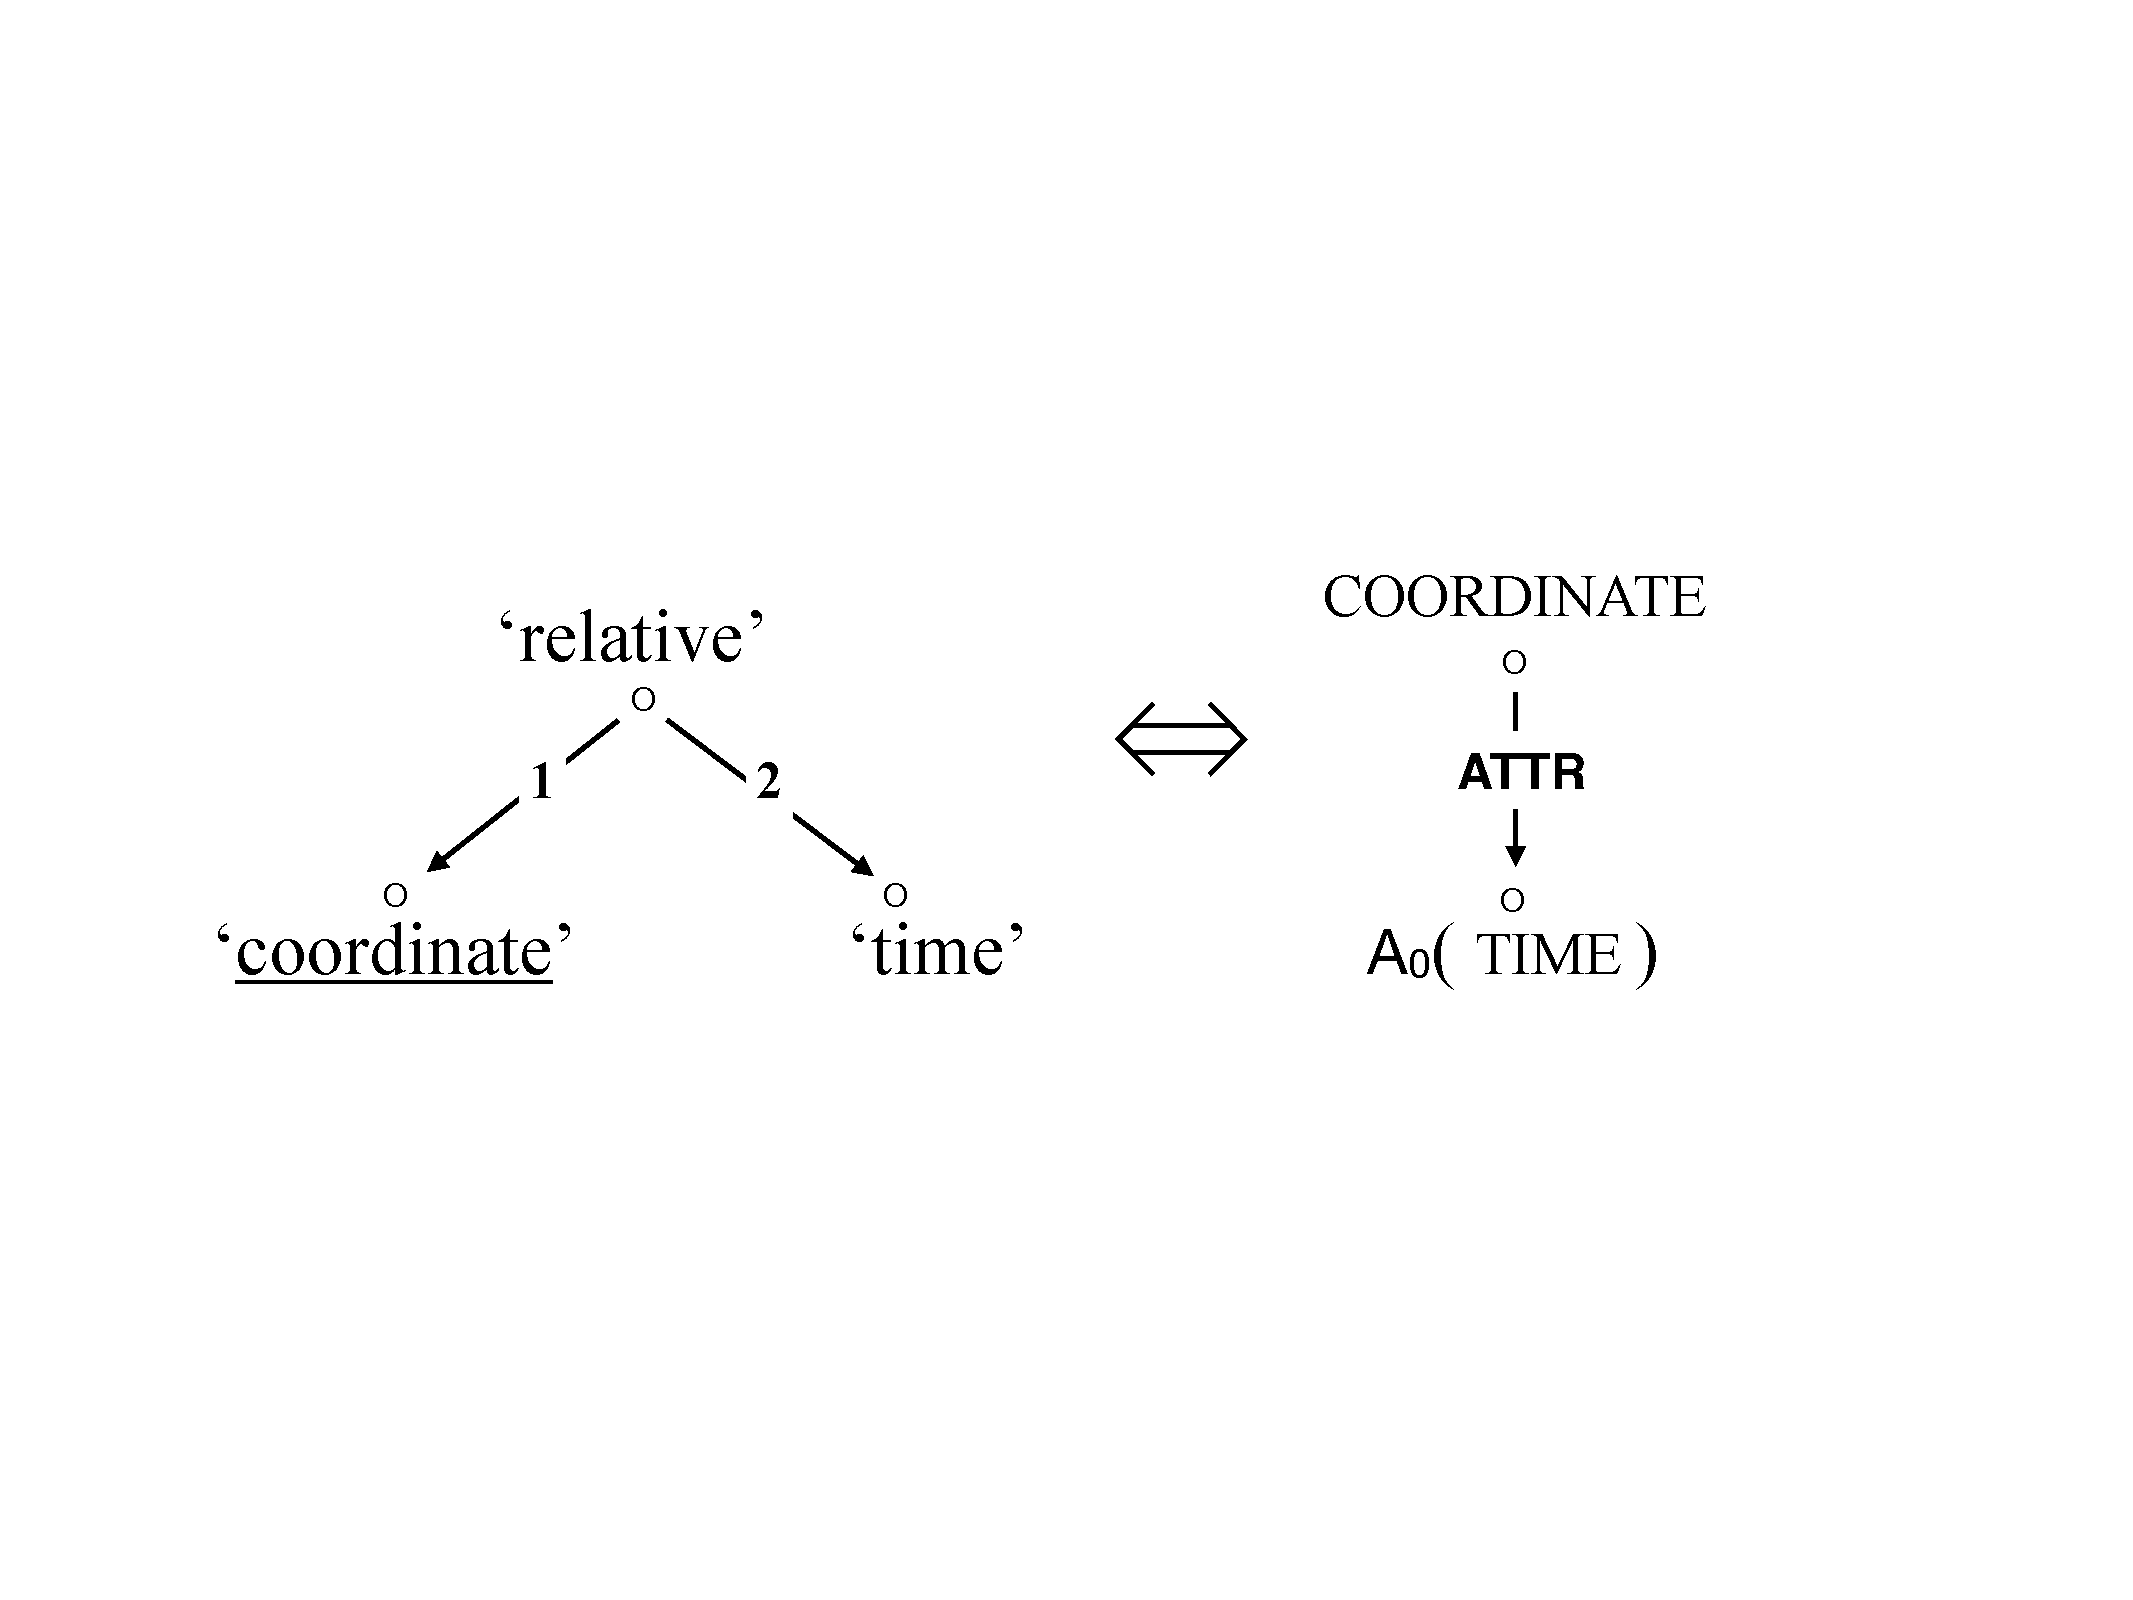
\includegraphics[width=7.3cm]{Fig/ParaLF/SemSyntA0.pdf}
\caption{Semantic content carried by an \lf{A\tsub{0}} syntactic modifier}\label{fig:Ch5-valeurSensA0}
\end{figure}

The semanteme `relative \lfgp{to}' is always included in the meaning of \lf{A\tsub{0}}. Given this semantic increment, it is not the case that \textsc{time}\tsub{(N)} is \lf{S\tsub{0}} of \textsc{temporal}; the \lf{S\tsub{0}} of \textsc{temporal} is \textsc{temporality}. The correspondences between these three lexemes are illustrated in paraphrases\index[notion]{paraphrase} \Next[a--c].

\begingroup
\small

\ex. \a. We measure the dimension of existence relative to \emph{time}.
     \b. We measure the \emph{temporal} dimension of existence.
     \c. We measure the dimension of existence relative to its \emph{temporality}.

\endgroup

The LF that associates \textsc{temporal} to \textsc{temporality} is called \lf{A\tsub{1}} -- an adjective characterizing the first deep-syntactic actant of L (that is, of \textsc{temporality}): \lfappl{A\tsub{1}}{\textsc{temporality}} = \textsc{temporal}. The LF \lf{A\tsub{1}} is presented below (\sectref{sec:derivAdjAct}, [\ref{lf:A-i}], p.\thinspace\pageref{lf:A-i}).

The lexical triplet {\scshape time}\tsub{(N)}, {\scshape temporal} and {\scshape temporality} forms a configuration of lexical links that is visualized in \figref{fig:configA0S0A1}. This type of configuration is highly recurrent in the lexical network\index[notion]{lexical network}\index[notion]{network \lfgp{see also \textit{graph}}!lexical \tld} of English and other languages.

\begin{figure}

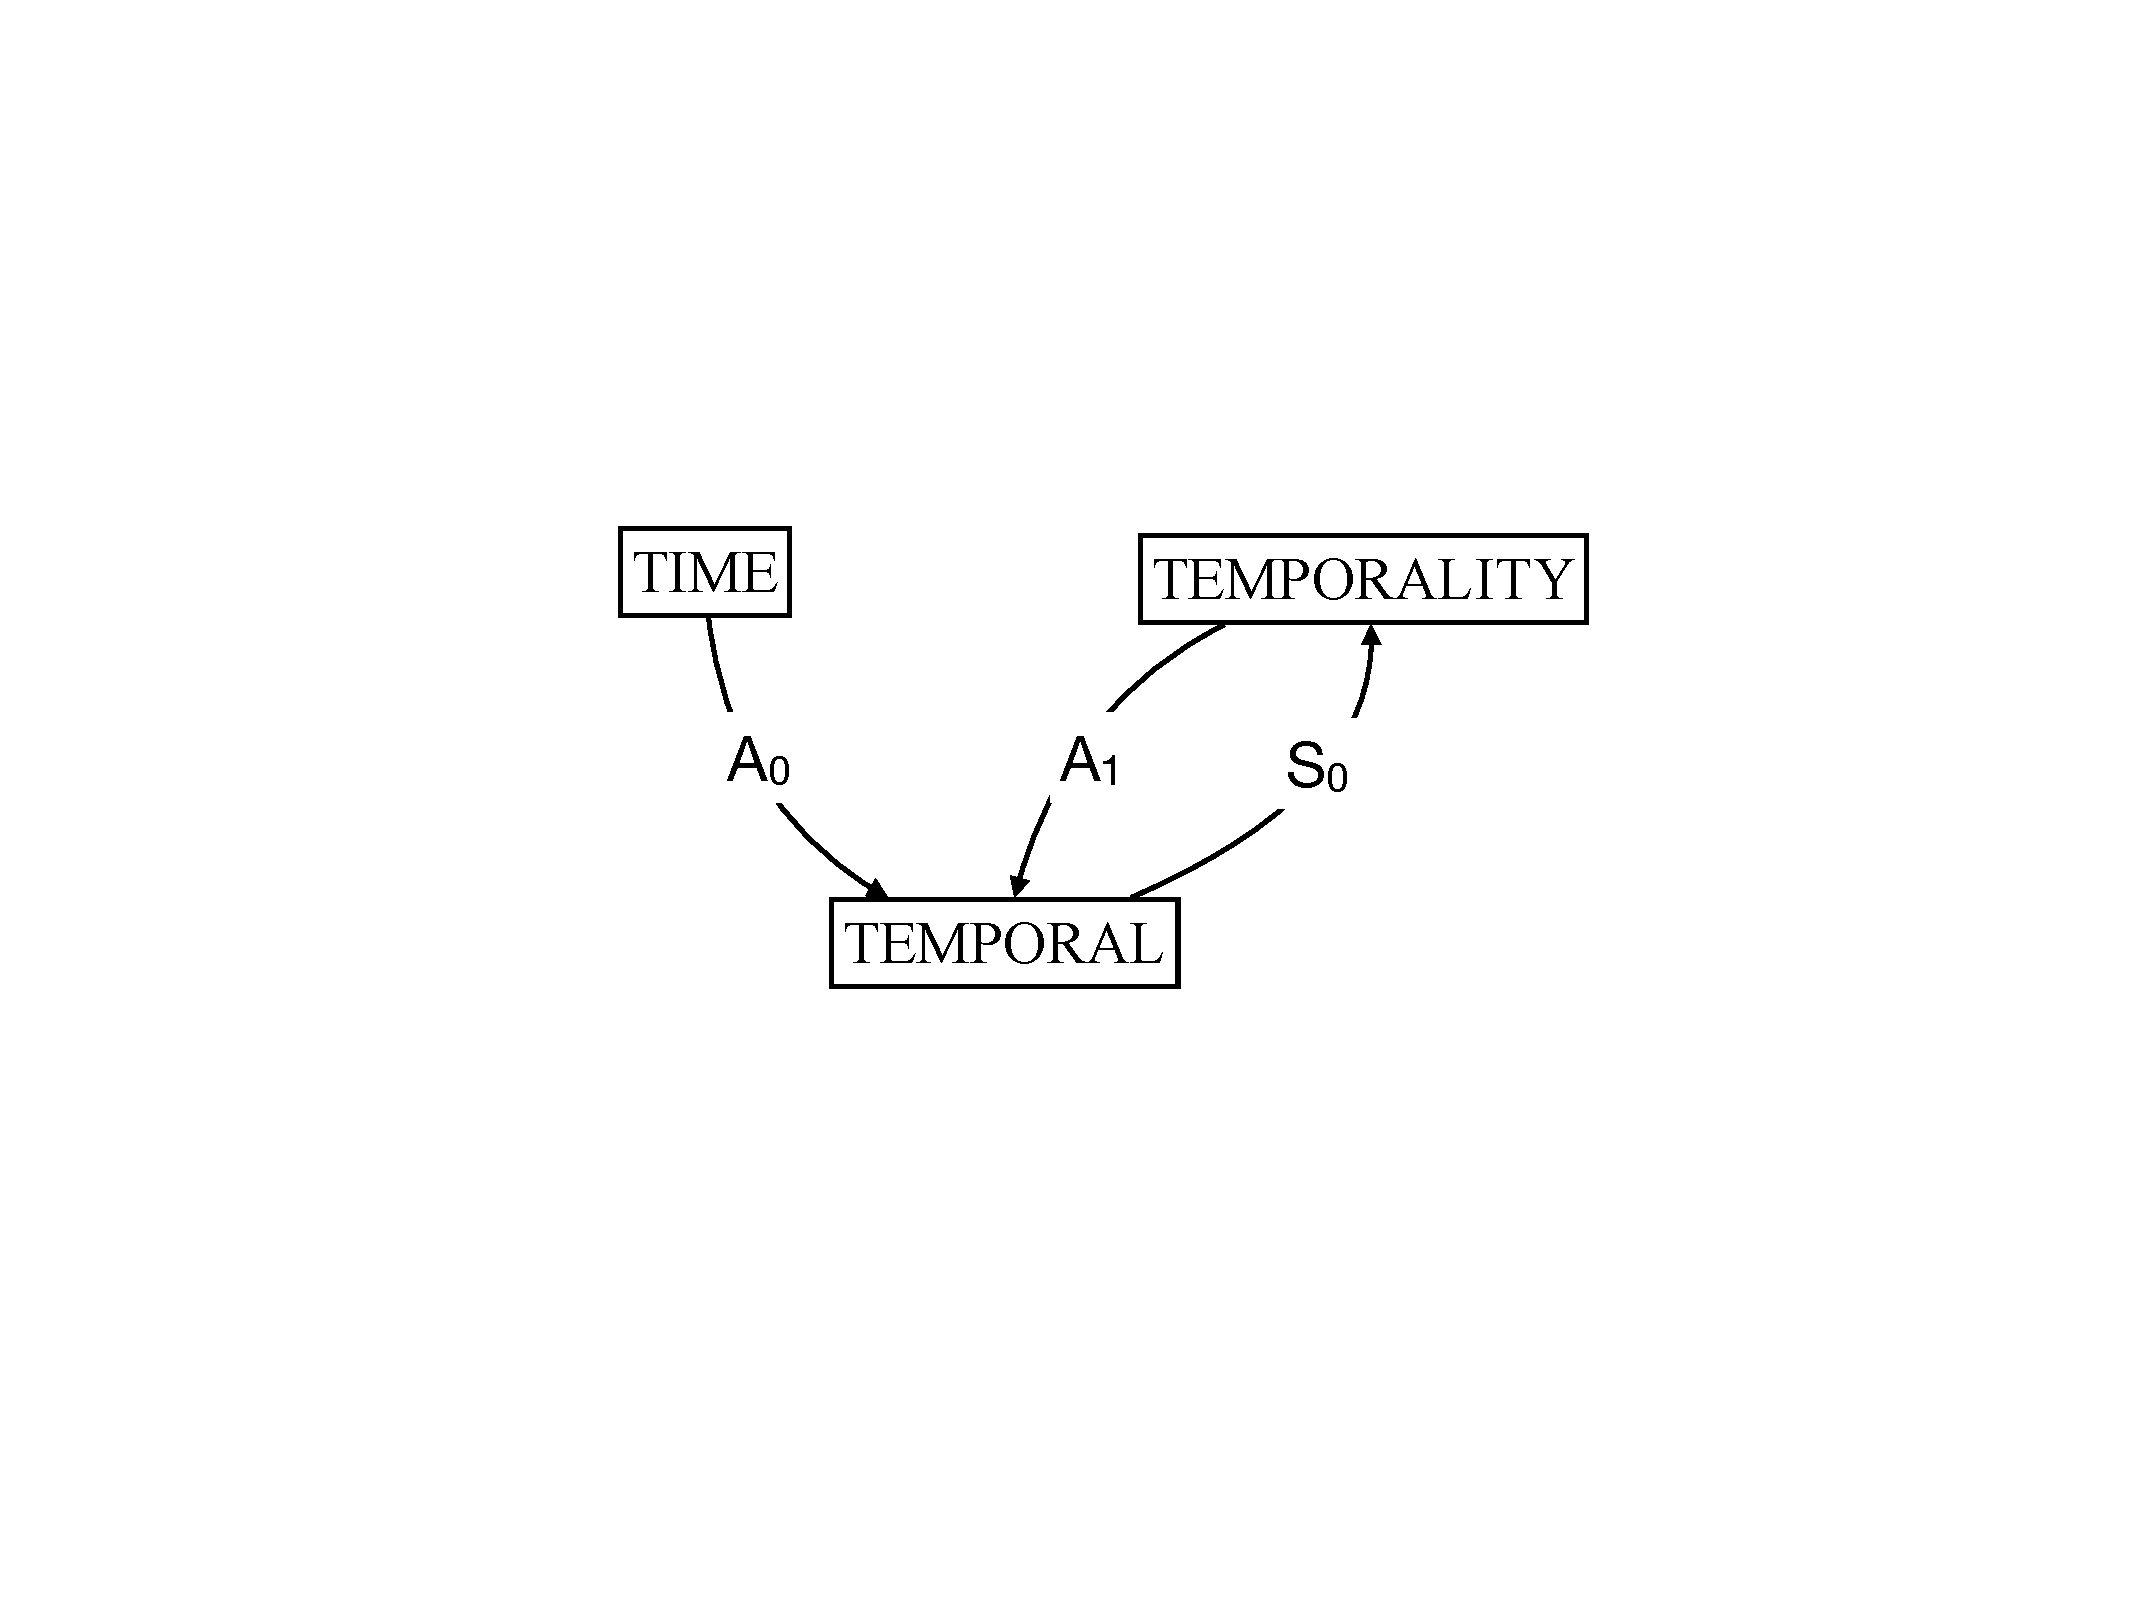
\includegraphics[width=4.7cm]{Fig/ParaLF/configA0S0A1.pdf}
\caption{Typical configuration of lexical links for \lf{A\tsub{0}} $\sim$ \lf{S\tsub{0}} $\sim$  \lf{A\tsub{1}}}\label{fig:configA0S0A1}
\end{figure}

\refstepcounter{LFlist}
\subsubsection*{{\small [\arabic{LFlist}]} \lf{Adv\tsub{0}} \lfgp{{\scriptsize Latin} \textit{adverbium}}: adverbialization}\label{lf:Adv0}
\addcontentsline{toc}{subsection}{{\footnotesize [\arabic{LFlist}]} \lf{Adv\tsub{0}}: adverbialization}\index[lf]{Adv0@\lf{Adv\tsub{0}}|emph}

\lf{Adv\tsub{0}} applies to a non-adverbial lexical unit L and returns an adverb\index[notion]{adverb} having the same meaning as L.

\begin{quote}
\begingroup
\small
\begin{tabular}{ l c c c c}
   \midrule
   \multicolumn{5}{l}{\lf{Adv\tsub{0}}: adverbial} \\
   \midrule
   \textbf{L} & V & N & Adj & Claus \\
   \midrule
   \textbf{\lfappl{Adv\tsub{0}}{L}} & Adv & Adv & Adv & Adv \\
   \midrule
\end{tabular}
\endgroup
\end{quote}

\begin{longtable*}[l]{ l l >{\raggedright\arraybackslash}p{7cm} }

\multicolumn{3}{l}{\textbf{English}} \\*

\lfappl{Adv\tsub{0}}{\textit{see}\tsub{(V)}} & = & \textit{visually} \lfgp{\textit{horrible to see}\enskip$\equiv$\enskip\textit{visually horrible}}  \\
\lfappl{Adv\tsub{0}}{\textit{vision}} & = & \textit{visually}  \\
\lfappl{Adv\tsub{0}}{\textit{alphabet}} & = & \textit{alphabetically}  \\
\lfappl{Adv\tsub{0}}{\textit{rapid}\tsub{(Adj)}} & = & \textit{rapidly}  \\*
\lfappl{Adv\tsub{0}}{\textit{close}\tsub{(Adj)}} & = & \textit{closely}\vspace{6pt}  \\

\multicolumn{3}{l}{\textbf{French}} \\*

\lfappl{Adv\tsub{0}}{\textit{voir}} &= & \textit{visuellement} \lfgp{\textit{insupportable à voir}\enskip$\equiv$\enskip\textit{visuellement insupportable}} \\
\lfappl{Adv\tsub{0}}{\textit{vue}} &= & \textit{visuellement} \\
\lfappl{Adv\tsub{0}}{\textit{alphabet}} &= & \textit{alphabétiquement} \\
\lfappl{Adv\tsub{0}}{\textit{rapide}\tsub{(Adj)}} &= & \textit{rapidement} \\
\lfappl{Adv\tsub{0}}{\textit{proche}} &= & \textit{près}\vspace{6pt} \\

\multicolumn{3}{l}{\textbf{Russian}} \\*

\lfappl{Adv\tsub{0}}{\textit{videt\palati}} & = & \idiom{\textit{na vid}} \lfgp{\textit{protivno videt}\enskip$\equiv$\enskip\textit{protivnyj \idiom{na vid}}} \\
\lfappl{Adv\tsub{0}}{\textit{zrenie}} & = & \textit{zritel\palati{}no} \\
\lfappl{Adv\tsub{0}}{\textit{alfavit}} & = & \textit{po alfavitu} \\
\lfappl{Adv\tsub{0}}{\textit{bystryj}} & = & \textit{bystro} \\*
\lfappl{Adv\tsub{0}}{\textit{blizkij}} & = & \textit{blizko} \\

\end{longtable*}

\lf{Adv\tsub{0}} should not be mistaken for another adverbialization LF, namely \lf{Adv\tsub{i}}\index[lf]{Advi@\lf{Adv\tsub{i}}}, which is examined below (\sectref{sec:derivAdvAct}, [\ref{lf:Adv-i}], p.\thinspace\pageref{lf:Adv-i}):

\begingroup
\small

\ex. \begingroup\setlength{\tabcolsep}{2pt}
\begin{tabular}[t]{ l l l >{\raggedright\arraybackslash}p{7cm} }
{\smaller English} & \lfappl{Adv\tsub{1}}{\textit{see} \lfgp{N\tsub{Y}}} &= & \textit{at the sight} \lfgp{\textit{of} N\tsub{Y}}\quad ($\equiv$\enskip\textit{seeing} \lfgp{N\tsub{Y}})  \\
{\smaller French} & \lfappl{Adv\tsub{1}}{\textit{voir} \lfgp{N\tsub{Y}}} &= & \textit{à la vue} \lfgp{\textit{de} N\tsub{Y}}  \\
{\smaller Russian} & \lfappl{Adv\tsub{1}}{\textit{videt\palati} \lfgp{N\tsub{Y-\textsc{acc}}}} &= & \textit{pri vide} \lfgp{N\tsub{Y-\textsc{gen}}}  \\
\end{tabular}\endgroup

\endgroup

\refstepcounter{LFlist}
\subsubsection*{{\small [\arabic{LFlist}]} \lf{Claus\tsub{0}} \lfgp{{\scriptsize Latin} *\textit{clausativum}}: clausativization}\label{lf:Claus0}
\addcontentsline{toc}{subsection}{{\footnotesize [\arabic{LFlist}]} \lf{Claus\tsub{0}}: clausativization}\index[lf]{Claus0@\lf{Claus\tsub{0}}|emph}

\lf{Claus\tsub{0}} applies to a non-clausative\index[notion]{clausative} lexical unit L and returns a clausative having the same meaning as L.

\lfappl{Claus\tsub{0}}{L} is a clausative lexical entity -- that is, a lexical entity syntactically equivalent to a sentence (cf. \chapref{chap:NotionLF}, \sectref{sec:notionPdD}, p.\thinspace\pageref{txt:Claus0}). \lf{Claus\tsub{0}} turns the meaning of its lexical argument L into the meaning of an utterance communicatively dominated\index[notion]{communicative!\tld\ dominance} by the semantic component `I signal \lfgp{that L ...}'. In this respect, \lf{Claus\tsub{0}} is not a pure structural derivation, just like \lf{A\tsub{0}}\index[lf]{A0@\lf{A\tsub{0}}} (see above, p.\thinspace\pageref{txt:A0NonPurelyStructural}); it adds a piece of communicative information (`I signal \lfgp{that L ...}') to the derivative.

\begin{soundbox}{To signal vs. to communicate}
\index[notion]{signal, to}\notion{To signal} is a term \parencite[249--250]{Melcuk2001b}: in contrast to \notion{to communicate}, it denotes an enunciation mode that precludes negation and interrogation. A signaled expression does not state something about the world, but manifests an internal (mental, emotional or physiological) state of the Speaker.
\end{soundbox}

\begin{quote}
\begingroup
\small
\begin{tabular}{l c c c c }
   \midrule
   \multicolumn{5}{l}{\lf{Claus\tsub{0}}: clausative} \\
   \midrule
   \textbf{L} & V & N & Adj & Adv \\
   \midrule
   \textbf{\lfappl{Claus\tsub{0}}{L}} & Claus & Claus & Claus & Claus \\
   \midrule
\end{tabular}
\endgroup
\end{quote}

\lf{Claus\tsub{0}} should not be mistaken for the \lf{Imper}\index[lf]{Imper@\lf{Imper}} LF (\sectref{sec:flFlexion}, [\ref{lf:Imper}], p.\thinspace\pageref{lf:Imper}), whose values are syntactically also clausatives, but which carry an additional meaning: `I signal that \emph{I want you to do} [L]'. 

\begin{longtable*}[l]{ l l >{\raggedright\arraybackslash}p{7cm} }

\multicolumn{3}{l}{\textbf{English}} \\*

\lfappl{Claus\tsub{0}}{\textit{congratulations}} & = & \textit{Congratulations!}\textbf{,} \textit{Congrats!} \\
\lfappl{Claus\tsub{0}}{\textit{meow}\tsub{(V)}} & = & \textit{Meow!} \\
\lfappl{Claus\tsub{0}Son}{\textit{cat}} & = & \textit{Meow!} \vspace{2pt}\\*
\multicolumn{3}{ p{11cm} }{\leftskip=0.5cm{\small\remark{Note.}For the LF \lf{Son}, see \chapref{chap:syntLFs}, [\ref{lf:Son}], p.\thinspace\pageref{lf:Son}.}} \vspace{2pt}\\
%\lfappl{Claus\tsub{0}Son}{\textit{chute}} & = & \textit{Badaboum !} \\
\lfappl{Claus\tsub{0}}{\textit{explosion}} & = & \textit{Boom!} \\
\lfappl{Claus\tsub{0}}{\textit{gunshot}} & = & \textit{Bang!}\textbf{,} \textit{Pow!} \\
\lfappl{Claus\tsub{0}}{\uslabel{informal} \textit{yucky}} & = & \textit{Yuck!}\vspace{6pt} \\

\multicolumn{3}{l}{\textbf{French}} \\*

\lfappl{Claus\tsub{0}}{\textit{féliciter}} & = & (\textit{Mes}) \textit{Félicitations !}\textbf{;} \textit{Chapeau !} \\
\lfappl{Claus\tsub{0}}{\textit{miauler}} & = & \textit{Miaou !} \\
\lfappl{Claus\tsub{0}Son}{\textit{chat}} & = & \textit{Miaou !} \\
\lfappl{Claus\tsub{0}Son}{\textit{chute}} & = & \textit{Badaboum !} \\
\lfappl{Claus\tsub{0}}{\textit{explosion}} & = & \textit{Boum !} \\
\lfappl{Claus\tsub{0}}{\idiom{\textit{coup de feu}}} & = & \textit{Pan !} \\
\lfappl{Claus\tsub{0}}{\textit{dégoûtant}} & = & \textit{Beurk !}\vspace{6pt} \\

\multicolumn{3}{l}{\textbf{Russian}} \\*

\lfappl{Claus\tsub{0}}{\textit{pozdravlenije}} & = & \textit{Pozdravljaju!} \\
\lfappl{Claus\tsub{0}}{\textit{mjaukat\palati}} & = & \textit{Mjau!} \\
\lfappl{Claus\tsub{0}Son}{\textit{ko\v{s}ka}} & = & \textit{Mjau!} \\
\lfappl{Claus\tsub{0}Son}{\textit{padenie}} & = & \textit{Bax!} \\
\lfappl{Claus\tsub{0}}{\textit{vystrel}} & = & \uslabel{child language} \textit{Pif-paf!} \\
\lfappl{Claus\tsub{0}}{\textit{protivnyj}} & = & \textit{Fi!}\textbf{;} \textit{Fu!} \\

\end{longtable*}

\begin{historicalremark}
The \lf{Claus\tsub{0}} LF was introduced in \textcite{MelcukPolguere2021} in order to better dovetail the set of structural derivative LFs with that of deep parts of speech\index[notion]{part of speech [PoS]!deep \tld}. \lf{Claus\tsub{0}} cancels the neological LF \lf{Enun}\index[lf]{Enun@\lf{Enun} \lfgp{no longer used}} ({\smaller Latin} \textit{\={e}nunti\={a}tus}), which was used in the \notion{DiCo}\index[notion]{lexical database!DiCo}\index[notion]{DiCo} lexicographic\index[notion]{lexicography} project\index[notion]{lexicography} \parencite{Polguere2000b}.
\end{historicalremark}

\section{Predicative derivatives}\label{sec:derivationPredicativisation}

\refstepcounter{LFlist}
\subsubsection*{{\small [\arabic{LFlist}]} \lf{Pred} \lfgp{{\scriptsize Latin} *\textit{praedic\={a}tum} `[a] predicate'}: predicativization}\label{lf:Pred}
\addcontentsline{toc}{subsection}{{\footnotesize [\arabic{LFlist}]} \lf{Pred}: predicativization}\index[lf]{Pred@\lf{Pred}|emph}

\lfappl{Pred}{L} is a verbal lexical unit that means `be\tsub{(copul)}~L'; it serves to turn a predicative\index[notion]{predicativity} noun, an adjective or an adverb L into a verb. Thus, \lf{Pred} plays the role of the copula\index[notion]{copula verb}\index[notion]{verb!copula \tld}; it is the paradigmatic counterpart of the syntagmatic LF \lf{Copul}\index[notion]{lexical function!paradigmatic vs. syntagmatic \tlds} (\chapref{chap:syntLFs}, [\ref{lf:Copul}], p.\thinspace\pageref{lf:Copul}).

Note that for adjectives and adverbs, the LF \lf{Pred} is semantically equivalent to \lf{V\tsub{0}}\index[lf]{V0@\lf{V\tsub{0}}} (see above, [\ref{lf:V0}], p.\thinspace\pageref{lf:V0}):

\begingroup
\small

\ex. \lfappl{Pred}{\textit{unexpected}}\thinspace=\thinspace\lfappl{V\tsub{0}}{\textit{unexpected}} \thinspace=\thinspace \idiom{\textit{come as a bolt from the blue}}

\endgroup

For quasi-predicative\index[notion]{predicate, semantic!quasi-\tld}\index[notion]{quasi-predicate} nouns denoting Agents\index[notion]{Agent (semantic role)!\tld\ noun}, \lf{Pred} is semantically equivalent to \lf{Fact\tsub{0}}\index[lf]{Facti@\lf{Fact\tsub{i}}!\lf{Fact\tsub{0}}} (\chapref{chap:syntLFs}, [\ref{lf:Fact-i}], p.\thinspace\pageref{txt:Fact0Descr}):

\begingroup
\small

\ex. \lfappl{Pred}{\textit{cook}\tsub{(N)}}\thinspace=\thinspace\lfappl{Fact\tsub{0}}{\textit{cook}\tsub{(N)}} \thinspace=\thinspace \textit{cook}\tsub{(V)} {\small `be a cook'}

\endgroup

\begin{quote}
\begingroup
\small
\begin{tabular}{ l c c c }
   \midrule
   \multicolumn{4}{l}{\lf{Pred}: verbal} \\
   \midrule
   \textbf{L} & N\tsub{(predic)} & Adj & Adv \\
   \midrule
   \textbf{\lfappl{Pred}{L}} & V & V & V \\
   \midrule
\end{tabular}
\endgroup
\end{quote}

\begin{longtable*}[l]{ l l >{\raggedright\arraybackslash}p{7cm} }

\multicolumn{3}{l}{\textbf{English}} \\*

\lfappl{Pred}{\textit{beggar}} & = & \textit{beg} {\small `be a beggar'} \lfgp{\textit{He begs for a living.}} \\
\lfappl{Pred}{\textit{cook}\tsub{(N)}} & = & \textit{cook}\tsub{(V)} {\small `be a cook'} \lfgp{\textit{He cooks in a posh restaurant.}} \\
\lfappl{Pred}{\textit{unexpected}} & = & \idiom{\textit{come as a bolt from the blue}} \\
\lfappl{Pred}{\textit{inseparable}} & = & \idiom{\textit{be joined at the hip}} \vspace{6pt} \\

\multicolumn{3}{l}{\textbf{French}} \\*

\lfappl{Pred}{\textit{mendiant}} & = & \textit{mendier} \\
\lfappl{Pred}{\textit{cuisinier}} & = & \textit{cuisiner} \\
\lfappl{Pred}{\textit{aisé} \lfgp{financièrement}} &= & \idiom{\textit{avoir les moyens}} \\
\lfappl{Pred\tsub{$\supset$}}{\textit{riche}\tsub{(Adj)}} &= & \uslabel{colloquial} \idiom{\textit{péter dans la soie}} \\
\lfappl{Pred}{\textit{inséparables}\tsub{(Adj)}} & = & \idiom{\textit{être comme les} (\textit{cinq}) \textit{doigts de la main}}\textbf{,} \\
 & & \idiom{\textit{être comme les deux doigts de la main}} \vspace{6pt} \\

\multicolumn{3}{l}{\textbf{Russian}} \\*

\lfappl{Pred}{\textit{ni\v{s}\v{c}ij}} & = & \textit{ni\v{s}\v{c}enstvovat\palati} \\
\lfappl{Pred}{\textit{direktor}} & = & \textit{direktorstvovat\palati} \\
\lfappl{Pred\tsub{$\supset$}}{\textit{bogatyj}} &= & \idiom{\textit{katat\palati{}sja kak syr v masle}} \\
\lfappl{Pred}{\textit{neo\v{z}idannyj}} & = & \uslabel{literary} \idiom{\textit{pojavit\palati{}sja kak \v{c}ërt iz tabakerki}} \\
\lfappl{Pred}{\textit{nerazlu\v{c}ny}} & = & \uslabel{colloquial} \idiom{\lfgp{N\tsub{X-\textsc{acc}}} \textit{vodoj ne razol\palati{}ë\v{s}\palati}} \\

\end{longtable*}

\paragraph*{\lf{Pred} in configurational\slashs complex LFs.}\index[notion]{lexical function!complex \tld}\index[notion]{lexical function!configurational \tld}\index[notion]{complex LF}\index[notion]{configurational LF}

\lf{Pred} is mostly combined with adjectival\slashs{}adverbial LFs \lf{Magn}\index[lf]{Magn@\lf{Magn}}, \lf{Ver}\index[lf]{Ver@\lf{Ver}} and \lf{Bon}\index[lf]{Bon@\lf{Bon}} (\chapref{chap:syntLFs}, \sectref{sec:collocatifsModif}, [\ref{lf:Magn}\slashs\ref{lf:Ver}\slashs\ref{lf:Bon}], p.\thinspace\pageref{lf:Magn}) to form configurational or complex LFs.

\begingroup
\small

\ex. \begingroup\setlength{\tabcolsep}{2pt}
\begin{tabular}[t]{ l l l >{\raggedright\arraybackslash}p{4.5cm} }
{\smaller English} & \lfappl{Magn+Pred}{\textit{angry}} & = & \textit{fume}\tsub{(V)} \\
{\smaller English} & \lfappl{Magn+Pred}{\textit{hungry}} & = & \textit{starve} \\
{\smaller French} & \lfappl{Magn+Pred}{\textit{chauve}\tsub{(N)} {\small `bald person'}} & = & \uslabel{vulgar} $\ulcorner$\textit{\begin{otherlanguage}{french}avoir une perruque en peau de fesse\end{otherlanguage}}$\urcorner$ {\footnotesize lit. `have a buttock-skin wig'} \\
{\smaller English} & \lfappl{PredMagn}{\textit{animosity}} = & & \\
 & \lfappl{Magn+Func\tsub{0}}{\textit{animosity}} & = & \idiom{\textit{run rampant}} \\
{\smaller English} & \lfappl{PredVer}{\textit{dress}\tsub{(N)}} & = & \textit{fit}\tsub{(V)}\textbf{;} \idiom{\textit{sit well}} \lfgp{\textit{with} N} \\
%\textrm{French} & \lfappl{Bon+Pred}{\textit{temps} {\scriptsize `weather'}} & = & \idiom{\textit{faire beau}} \\
\end{tabular}\endgroup

\endgroup

Note that cases of the configurational \emph{paradigmatic}\index[notion]{lexical function!paradigmatic vs. syntagmatic \tlds} LF \lf{Magn+Pred} were mistakenly described as cases of the complex \emph{syntagmatic} LF \lf{PredMagn} in \textcite[216--217]{Melcuk2015a-e}.

For more on the use of \lf{Pred} in complex LFs, see the description of the syntagmatic LF \lf{Plus}\index[lf]{Plus@\lf{Plus}} (\chapref{chap:syntLFs}, [\ref{lf:Plus}], p.\thinspace\pageref{lf:Plus}).

\section{Nominal derivatives}\label{sec:derivNom}

Nominal derivatives fall into two classes: actantial (\sectref{sec:derivNomAct}) vs. circumstantial (\sectref{sec:derivNomCirc}). Note that adjectival (\sectref{sec:derivAdjAct}) and adverbial (\sectref{sec:derivAdvAct}) derivatives are only actantial.

\subsection{Nominal actantial derivatives}\label{sec:derivNomAct}

This section presents, in the first place, the LFs \lf{S\tsub{1}}, \lf{S\tsub{2}}, \lf{S\tsub{3}}, ... -- for short, \lf{S\tsub{i}}. \lf{S\tsub{i}} applies to a predicative lexical unit\index[notion]{predicativity} -- predicate\index[notion]{predicate, semantic} or quasi-predicate\index[notion]{predicate, semantic!quasi-\tld} -- and returns the name for its DSyntA\thinspace\syntDname{I}, \syntDname{II}, \syntDname{III}, ...

Also included in this section are two more specific LFs intimately related to \lf{S\tsub{i}}: \lf{Equip} and \lf{Cap}.

\refstepcounter{LFlist}
\subsubsection*{{\small [\arabic{LFlist}]} \lf{S\tsub{i}}: typical name for L's DSyntA\thinspace\syntDname{i}}\label{lf:S-i}
\addcontentsline{toc}{subsection}{{\footnotesize [\arabic{LFlist}]} \lf{S\tsub{i}}: typical name for L's DSyntA\thinspace\syntDname{i}}\index[lf]{Si@\lf{S\tsub{i}}|emph}

\lfappl{S\tsub{i}}{L} is a nominal lexical entity that is the name for L's DSyntA\thinspace\syntDname{I}, \syntDname{II}, \syntDname{III}, ...

\begin{quote}
\begingroup
\small
\begin{tabular}{ l  c c c c c }
   \midrule
   \multicolumn{6}{l}{\lf{S\tsub{i}}: nominal} \\
   \midrule
   \textbf{L} & V & N & Adj & Adv & Claus \\
   \midrule
   \textbf{\lfappl{S\tsub{i}}{L}} & N & N & N & N & N\\
   \midrule
\end{tabular}
\endgroup
\end{quote}

\begin{longtable*}[l]{ l l >{\raggedright\arraybackslash}p{7cm} }

\multicolumn{3}{l}{\textbf{English}} \\*

\lfappl{S\tsub{1}}{\textit{sell}\tsub{(V)}} & = & \textit{seller} \\
\multicolumn{3}{l}{\quad\lfgp{N\tsub{X} \textit{sells} N\tsub{Y} \textit{to} N\tsub{Z} \textit{for} N\tsub{W}}} \\
\lfappl{S\tsub{2}}{\textit{sell}\tsub{(V)}} & = & \textit{merchandise} \\
\lfappl{S\tsub{3}}{\textit{sell}\tsub{(V)}} & = & \textit{buyer} \\
\lfappl{S\tsub{4}}{\textit{sell}\tsub{(V)}} & = & \textit{price} \\
\lfappl{S\tsub{1}}{\textit{chemistry}} & = & \textit{chemist} \\
\multicolumn{3}{l}{\quad\lfgp{\textit{chemistry done by} N\tsub{X}}} \\
\lfappl{S\tsub{1}}{\textit{mute}\tsub{(Adj)}} & = & \textit{mute}\tsub{(N)} \\
\multicolumn{3}{l}{\quad\lfgp{N\tsub{X} \textit{is mute}}} \\
\lfappl{S\tsub{1}}{\textit{lazy}} & = & \uslabel{colloquial} \textit{lazybones} \\
\multicolumn{3}{l}{\quad\lfgp{N\tsub{X} \textit{is lazy}}}\vspace{6pt} \\

\multicolumn{3}{l}{\textbf{French}} \\*

\lfappl{S\tsub{1}}{\textit{vendre}} & = & \textit{vendeur} \\
\lfappl{S\tsub{2}}{\textit{vendre}} & = & \textit{marchandise} \\
\lfappl{S\tsub{3}}{\textit{vendre}} & = & \textit{acheteur} \\
\lfappl{S\tsub{4}}{\textit{vendre}} & = & \textit{prix} \\
\lfappl{S\tsub{1}}{\textit{chimie}} & = & \textit{chimiste} \\
\lfappl{S\tsub{1}}{\textit{muet}\tsub{(Adj)}} & = & \textit{muet}\tsub{(N)}\vspace{6pt} \\
%\lfappl{S\tsub{2}}{\textit{À bas} \lfgp{N\tsub{Y}} \textit{!}} & = & \textit{ennemi} \\

\multicolumn{3}{l}{\textbf{Russian}} \\*

\lfappl{S\tsub{1}}{\textit{prodavat\palati}} & = & \textit{prodavec} \\
\lfappl{S\tsub{2}}{\textit{prodavat\palati}} & = & \textit{tovar} \\
\lfappl{S\tsub{3}}{\textit{prodavat\palati}} & = & \textit{pokupatel\palati} \\
\lfappl{S\tsub{4}}{\textit{prodavat\palati}} & = & \textit{cena} \\
\lfappl{S\tsub{1}}{\textit{ximija}} & = & \textit{ximik} \\
\lfappl{S\tsub{1}}{\textit{nemoj}\tsub{(Adj)}} & = & \textit{\textit{nemoj}}\tsub{(N)} \\

\end{longtable*}

\refstepcounter{LFlist}
\subsubsection*{{\small [\arabic{LFlist}]} \lf{Equip} \lfgp{{\scriptsize French} \textit{équipage} `crew'}: team that allows L's referent\index[notion]{referent} to function}\label{lf:Equip}
\addcontentsline{toc}{subsection}{{\footnotesize [\arabic{LFlist}]} \lf{Equip}: team that allows L's referent to function}\index[lf]{Equip@\lf{Equip}|emph}

\lfappl{Equip}{L} is a nominal lexical entity that designates an organized set of individuals (or, more generally, of living beings) involved in the functioning of L's referent; in other words, \lfappl{Equip}{L} designates the set of L's DSyntAs~\syntDname{I}. Consequently, L is a quasi-predicative\index[notion]{predicate, semantic!quasi-\tld}\index[notion]{quasi-predicate} noun denoting a functioning entity\index[notion]{entity@`entity'}.

\begin{quote}
\begingroup
\small
\begin{tabular}{ l c }
   \midrule
   \multicolumn{2}{l}{\lf{Equip}: nominal} \\
   \midrule
   \textbf{L} & N  \\
   \midrule
   \textbf{\lfappl{Equip}{L}} & N \\
   \midrule
\end{tabular}
\endgroup
\end{quote}

\begin{longtable*}[l]{ l l >{\raggedright\arraybackslash}p{7cm} }

\multicolumn{3}{l}{\textbf{English}} \\*

\lfappl{Equip}{\textit{ship}\tsub{(N)}} & = & \textit{crew} \\
\lfappl{Equip}{\textit{theater}} & = & \textit{company} \\
\lfappl{Equip}{\textit{newspaper}} & = & \idiom{\textit{editorial staff}}\vspace{6pt} \\

\multicolumn{3}{l}{\textbf{French}} \\*

\lfappl{Equip}{\textit{navire}} & = & \textit{équipage} \\
\lfappl{Equip}{\textit{théâtre}} & = & \textit{troupe} \\
\lfappl{Equip}{\textit{journal}} & = & \textit{rédaction}\vspace{6pt} \\

\multicolumn{3}{l}{\textbf{Russian}} \\*

\lfappl{Equip}{\textit{sudno}} & = & \textit{èkipa\v{z}} \\
\lfappl{Equip}{\textit{teatr}} & = & \textit{truppa} \\
\lfappl{Equip}{\textit{gazeta}} & = & \textit{redakcija} \\

\end{longtable*}

\newpage
According to its nature, \lf{Equip} applies only to lexical units whose DSyntA\thinspace\syntDname{I} denotes a participant -- \lfappl{S\tsub{1}}{L} -- that makes the entity L function.  In other words, \lf{Equip} means `set of \lf{S\tsub{1}}'; compare the above English illustrations of \lf{Equip} with~\Next:

\begingroup
\small

\ex. \begingroup\setlength{\tabcolsep}{2pt}
\begin{tabular}[t]{ l l >{\raggedright\arraybackslash}p{7cm} }
\lfappl{S\tsub{1}}{\textit{ship}\tsub{(N)}} & = & \textit{sailor} \lfgp{(\textit{ship's}) \textit{crew}\enskip$\equiv$\enskip\textit{set of sailors}} \\
\lfappl{S\tsub{1}}{\textit{theater}} & = & \textit{actor} \lfgp{(\textit{theater's}) \textit{company}\enskip$\equiv$\enskip\textit{set of actors}} \\
\lfappl{S\tsub{1}}{\textit{newspaper}} & = & \textit{journalist} \lfgp{\idiom{\textit{editorial staff}}\enskip$\equiv$\enskip\textit{set of journalists}} \\
\end{tabular}\endgroup

\endgroup

The meaning `set [of Xs]' is represented by the LF \lf{Mult}\index[lf]{Mult@\lf{Mult}} (\sectref{sec:flFlexion}, [\ref{lf:Mult}], p.\thinspace\pageref{lf:Mult}). It is thus possible to propose a paraphrasing rule \textbf{R\tsub{\lf{Equip}}} that states the following semantic equivalence:

\begin{center}
\phantomsection\label{txt:RParaphEquip}\APolbox{8.5cm}{%
\renewcommand{\arraystretch}{1.1}
\begin{tabular}{ l l }
\textbf{R\tsub{\lf{Equip}}:} & \lfappl{Equip}{L}\enskip{\small$\equiv$}\enskip\lfappl{MultS\tsub{1}}{L} \\*
& {\small\textit{crew} \senseex{of a ship}\enskip$\equiv$\enskip\textit{set of sailors}\tsub{\lfappl{S$_\text{1}$}{\textit{ship}}} \senseex{of a ship}} \\
\end{tabular}
}
\end{center}\index[notion]{paraphrase!deep-syntactic paraphrasing rule!\textbf{R\tsub{\lf{Equip}}}|emph}

We can foresee a possible generalization of the LF \lf{Equip} in order to cover cases corresponding to \lf{MultS\tsub{2}}, \lf{MultS\tsub{3}}, etc. With such a generalization, it would be necessary to distinguish \lf{Equip\tsub{1}}, \lf{Equip\tsub{2}}, \lf{Equip\tsub{3}}, etc.

\refstepcounter{LFlist}
\subsubsection*{{\small [\arabic{LFlist}]} \lf{Cap} \lfgp{{\scriptsize Latin} \textit{caput} `head'}: person in charge of L's referent\index[notion]{referent}}\label{lf:Cap}
\addcontentsline{toc}{subsection}{{\footnotesize [\arabic{LFlist}]} \lf{Cap}: person in charge of L's referent}\index[lf]{Cap@\lf{Cap}|emph}

\lfappl{Cap}{L} is a nominal lexical entity that designates the individual in charge of a functioning entity L (in fact, in charge of the set of L's DSyntAs\thinspace\syntDname{I}). As for \lf{Equip}, L is a quasi-predicative\index[notion]{predicate, semantic!quasi-\tld}\index[notion]{quasi-predicate} noun.

\begin{quote}
\begingroup
\small
\begin{tabular}{ l c }
   \midrule
   \multicolumn{2}{l}{\lf{Cap}: nominal} \\
   \midrule
   \textbf{L} & N  \\
   \midrule
   \textbf{\lfappl{Cap}{L}} & N \\
   \midrule
\end{tabular}
\endgroup
\end{quote}

\lfappl{Cap}{L} denotes a specific element of the set of \lfappl{S\tsub{1}}{L}. Two cases have to be distinguished:

\begin{itemize}

\item if L denotes a group of individuals (e.g. a tribe, a pack of animals, etc.), \lfappl{Cap}{L} denotes the main member of this group;

\item if L denotes a functioning entity (e.g. a plane, a school, etc.) run by a group of individuals -- that is, run by \lfappl{Equip}{L}\index[lf]{Equip@\lf{Equip}}, \lfappl{Cap}{L} is the main member of \lfappl{Equip}{L}.

\end{itemize}

\begin{longtable*}[l]{ l l >{\raggedright\arraybackslash}p{7cm} }

\multicolumn{3}{l}{\textbf{English}} \\*

\lfappl{Cap}{\textit{kingdom}} & = & \textit{king} \\
\lfappl{Cap}{\textit{mafia}} & = & \textit{don}\textbf{,} \textit{godfather} \\
\lfappl{Cap}{\textit{ship}\tsub{(N)}} & = & \textit{captain}\sensenum{1} \\
\lfappl{Cap}{\textit{plane}\tsub{(N)}} & = & \textit{captain}\sensenum{2} \\
\lfappl{Cap}{\textit{school}\tsub{(N)}} & = & \textit{principal}\tsub{(N)} \\
\lfappl{Cap}{\textit{tribe}} & = & \textit{chief} (\textit{of} \textsc{art} \tld) \\
\lfappl{Cap}{\lfgp{\textit{wolf}} \textit{pack}\tsub{(N)}} & = & \textit{leader} (\textit{of} \textsc{art} \tld)\vspace{6pt} \\

\multicolumn{3}{l}{\textbf{French}} \\*

\lfappl{Cap}{\textit{royaume}} & = & \textit{roi} \\
\lfappl{Cap}{\textit{mafia}} & = & \textit{parrain} \\
\lfappl{Cap}{\textit{navire}} & = & \textit{capitaine}\sensenum{1} \\
\lfappl{Cap}{\textit{avion}} & = & \textit{capitaine}\sensenum{2}\textbf{,} \textit{commandant} (\textit{de bord}) \\
\lfappl{Cap}{\textit{gare}} & = & \idiom{\textit{chef de gare}} \\
\lfappl{Cap}{\textit{tribu}} & = & \textit{chef}\sensenum{1} (\textit{de} (\textsc{art}) \tld) \\
\lfappl{Cap}{\textit{meute}} & = & \textit{chef}\sensenum{2} (\textit{de} (\textsc{art}) \tld)\vspace{6pt} \\

\multicolumn{3}{l}{\textbf{Russian}} \\*

\lfappl{Cap}{\textit{korolevstvo}} & = & \textit{korol\palati} \\
\lfappl{Cap}{\textit{mafija}} & = & \textit{boss} \\
\lfappl{Cap}{\textit{sudno}} & = & \textit{kapitan} \\
\lfappl{Cap}{\textit{samolët}} & = & \idiom{\textit{komandir korablja}} \\
\lfappl{Cap}{\textit{plem\suffixsplit ja}} & = & \textit{vo\v{z}d\palati} (\tld\textit{eni}) \\
\lfappl{Cap}{\textit{sta\suffixsplit ja}} & = & \textit{vo\v{z}ak} (\tld\textit{i}) \\

\end{longtable*}

\subsection{Nominal circumstantial derivatives}\label{sec:derivNomCirc}\index[notion]{circumstantial}

As seen above, \lf{S\tsub{i}}\index[lf]{Si@\lf{S\tsub{i}}} applies to a predicative or quasi-predicative\index[notion]{predicate, semantic}\index[notion]{predicate, semantic!quasi-\tld}\index[notion]{quasi-predicate} lexical unit L and returns the general name for DSyntA\thinspace\syntDname{i} of L. In contrast, the next five LFs -- \lf{S\tsub{loc}}\index[lf]{Sloc@\lf{S\tsub{loc}}}, \lf{S\tsub{instr}}\index[lf]{Sinstr@\lf{S\tsub{instr}}}, \lf{S\tsub{med}}\index[lf]{Smed@\lf{S\tsub{med}}}, \lf{S\tsub{res}}\index[lf]{Sres@\lf{S\tsub{res}}} and \lf{S\tsub{mod}}\index[lf]{Smod@\lf{S\tsub{mod}}} -- return for L the name of L's prototypical \notion{circumstantials} (a.k.a. adverbials, or adjuncts): locative, instrumental, means, result and manner circumstantials.

The domain of application\index[notion]{domain of application of an LF}\index[notion]{application of an LF!domain of \tld}\index[notion]{lexical function!domain of application of a \tld} of a circumstantial LF is determined by its semantic content, namely:

\begin{itemize}

\item \lf{S\tsub{loc}} applies to an L that denotes either an entity or a fact (action, event, process, state, ...), since both entities and facts can have localizations;

\item \lf{S\tsub{instr}} and \lf{S\tsub{med}} apply to an L that denotes an action -- i.e. a particular type of fact, since only actions involve instruments and means;

\item \lf{S\tsub{res}} and \lf{S\tsub{mod}} take an L that denotes a dynamic fact (action, event, process): only dynamic facts have results and happen in a certain way.

\end{itemize}

Because of their particular semantic content, the circumstantial LFs do not apply to adjectives and adverbs. All circumstantial LFs have the same PoS table:

\begin{quote}
\begingroup
\phantomsection\label{exLvalPossible}\small
\begin{tabular}{ l c c c }
   \midrule
   \multicolumn{4}{l}{\lf{S\tsub{loc\slashs{}instr\slashs{}med\slashs{}res\slashs{}mod}}: nominal} \\
   \midrule
   \textbf{L} & V & N & Claus \\
   \midrule
   \textbf{\lfappl{S\tsub{loc\slashs{}instr\slashs{}med\slashs{}res\slashs{}mod}}{L}} & N & N & N \\
   \midrule
\end{tabular}
\endgroup
\end{quote}

The order\index[notion]{lexical function!ordering of \tlds}\index[notion]{ordering of LFs} of presentation of circumstantial LFs follows, roughly speaking, the hierarchy of circumstantials in natural languages: from more to less linguistically privileged circumstantials.

\begin{historicalremark}
A different ordering\index[notion]{lexical function!ordering of \tlds}\index[notion]{ordering of LFs} of circumstantial LFs was used in previous publications, namely: \lf{S\tsub{loc}}, instead of heading the enumeration, was arbitrarily placed in the penultimate position.
\end{historicalremark}

\refstepcounter{LFlist}
\subsubsection*{{\small [\arabic{LFlist}]} \lf{S\tsub{loc}} \lfgp{{\scriptsize Latin} \textit{locus} `place'}: name of the prototypical location}\label{lf:S-loc}
\addcontentsline{toc}{subsection}{{\footnotesize [\arabic{LFlist}]} \lf{S\tsub{loc}}: name of the prototypical location}\index[lf]{Sloc@\lf{S\tsub{loc}}|emph}

\lfappl{S\tsub{loc}}{L} is a nominal lexical entity that is the name of the prototypical location of the referent of L.

\begin{longtable*}[l]{ l l >{\raggedright\arraybackslash}p{6cm} }

\multicolumn{3}{l}{\textbf{English}} \\*

\lfappl{S\tsub{loc}}{\textit{surgery}} & = & \idiom{\textit{operation room}} \\
\lfappl{S\tsub{loc}}{\textit{smoke}\tsub{(V)}} & = & \idiom{\textit{smoking area}}\textbf{;} \idiom{\textit{smoking room}} \\
\lfappl{S\tsub{loc}}{\uslabel{formal} \textit{excrete}} & = & \textit{bathroom}\textbf{,} \textit{restroom}\textbf{,} \textit{toilet}\tsub{(N)}\textbf{,} \textit{washroom}\textbf{;} \textit{privy}\textbf{;} \textit{outhouse} \\
\lfappl{S\tsub{loc}}{\textit{orphan}} & = & \textit{orphanage} \\
\lfappl{S\tsub{loc}}{\textit{cattle}} & = & \textit{stable}\tsub{(N)}\vspace{6pt} \\

\multicolumn{3}{l}{\textbf{French}} \\*

\lfappl{S\tsub{loc}}{\textit{opération} \lfgp{chirurgicale}} & = & \idiom{\textit{salle d'opération}}\textbf{;} \idiom{\textit{bloc opératoire}} \\
\lfappl{S\tsub{loc}}{\textit{fumer}} & = & \textit{espace fumeur}(\textit{s})\textbf{;} \textit{fumoir} \\
\lfappl{S\tsub{loc}}{\idiom{\textit{faire ses besoins}}} & = & \uslabel{vulgar} \textit{chiottes}\textbf{,} \textit{toilettes}\textbf{,} \textit{W.-C.}\textbf{;} \uslabel{formal}~\idiom{\textit{lieu d'aisance}(\textit{s})}\textbf{;} \textit{latrine} \\
\lfappl{S\tsub{loc}}{\textit{orphelin}} & = & \textit{orphelinat} \\
\lfappl{S\tsub{loc}}{\textit{bétail}} & = & \textit{étable}\vspace{6pt} \\

\multicolumn{3}{l}{\textbf{Russian}} \\*

\lfappl{S\tsub{loc}}{\textit{operacija}} & = & \textit{operacionnaja} \\
\lfappl{S\tsub{loc}}{\textit{kurit\palati}} & = & \idiom{\textit{mesto dlja kurenija}}\textbf{,} \uslabel{colloquial}~\textit{kurilka} \\
\lfappl{S\tsub{loc}}{\uslabel{colloquial} \idiom{\textit{spravljat\palati nu\v{z}du}}} & = & \textit{tualet}\textbf{,} \textit{ubornaja}\textbf{;} \uslabel{colloquial}~\textit{sortir} \\
\lfappl{S\tsub{loc}}{\textit{sirota}} & = & \idiom{\textit{detskij dom}} \\
\lfappl{S\tsub{loc}}{\textit{skot}} & = & \textit{xlev} \\

\end{longtable*}

\refstepcounter{LFlist}
\subsubsection*{{\small [\arabic{LFlist}]} \lf{S\tsub{instr}} \lfgp{{\scriptsize Latin} \textit{instrumentum} `tool'}: name of the prototypical instrument}\label{lf:S-instr}
\addcontentsline{toc}{subsection}{{\footnotesize [\arabic{LFlist}]} \lf{S\tsub{instr}}: name of the prototypical instrument}\index[lf]{Sinstr@\lf{S\tsub{instr}}|emph}

\lfappl{S\tsub{instr}}{L} is a nominal lexical entity that is the name of the instrument, in the most general sense, which is prototypically used to do L.

\begin{longtable*}[l]{ l l >{\raggedright\arraybackslash}p{7cm} }

\multicolumn{3}{l}{\textbf{English}} \\*

\lfappl{S\tsub{instr}}{\textit{drink}\tsub{(V)}} & = & \textit{glass}\textbf{;} \textit{cup} \\
\lfappl{S\tsub{instr}}{\textit{shower}\tsub{(V)}} & = & \textit{shower}\tsub{(N)}\sensenum{II} \lfgp{equipment} \\
\lfappl{S\tsub{instr}}{\textit{wash}\tsub{(V)} \lfgp{oneself}} & = & \textit{washcloth} \\
\lfappl{S\tsub{instr}}{\textit{fry}\tsub{(V)}} & = & \idiom{\textit{frying pan}}\textbf{,} \textit{skillet}\textbf{;} \textit{fryer} \\
\lfappl{S\tsub{instr}}{\textit{smell}\tsub{(V)}} & = & \textit{nose}\tsub{(N)} \\
\lfappl{S\tsub{instr}}{\textit{murder}\tsub{(N)}} & = & \idiom{\textit{murder weapon}} \\
\lfappl{S\tsub{instr}}{\textit{Snip!}} & = & \textit{scissors}\vspace{6pt} \\

\multicolumn{3}{l}{\textbf{French}} \\*

\lfappl{S\tsub{instr}}{\textit{boire}} & = & \textit{verre}\textbf{;} \textit{tasse} \\
\lfappl{S\tsub{instr}}{\textit{se doucher}} & = & \textit{douche}\sensenum{II} \lfgp{equipment} \\
\lfappl{S\tsub{instr}}{\textit{se laver}} & = & \idiom{\textit{gant de toilette}} \\
\lfappl{S\tsub{instr}}{\textit{frire}} & = & \senseex{une} \textit{poêle}\textbf{;} \textit{friteuse} \\
\lfappl{S\tsub{instr}}{\textit{sentir}} & = & \textit{nez} \\
\lfappl{S\tsub{instr}}{\textit{crime}} & = & \idiom{\textit{arme du crime}} \\
\lfappl{S\tsub{instr}}{\textit{Glouglou !} } & = & \textit{verre}\vspace{6pt} \\

\multicolumn{3}{l}{\textbf{Russian}} \\*

\lfappl{S\tsub{instr}}{\textit{pit\palati}} & = & \textit{stakan}\textbf{;} \textit{\v{c}a\v{s}ka}\textbf{;} \textit{rjumka} \\
\lfappl{S\tsub{instr}}{\senseex{prinimat\palati} \textit{du\v{s}}\sensenum{I}} & = & \textit{du\v{s}}\sensenum{II} \lfgp{equipment}\\
\lfappl{S\tsub{instr}}{\textit{pri\v{c}ësyvat\palati{}sja}} & = & \textit{grebe\v{s}ok}\textbf{,} \textit{ras\v{c}ëska} \\
\lfappl{S\tsub{instr}}{\textit{\v{z}arit\palati}} & = & \textit{skovoroda}\textbf{;} \textit{fritjurnica} \\
\lfappl{S\tsub{instr}}{\textit{njuxat\palati}} & = & \textit{nos} \\
\lfappl{S\tsub{instr}}{\textit{prestuplenie}} & = & \idiom{\textit{orudie prestuplenija}} \\*
\lfappl{S\tsub{instr}}{\textit{\v{C}ik!}} & = & \textit{no\v{z}}\textbf{;} \textit{no\v{z}nicy} \\

\end{longtable*}

In the above examples, {\smaller English}~\textit{Snip!}, {\smaller French}~\textit{Glouglou !} and {\smaller Russian}~\textit{\v{C}ik!} are clausative\index[notion]{clausative} elements of the value of the LF \lf{Claus\tsub{0}SonS\tsub{0}} for the verbs {\smaller English}~\textit{cut}, {\smaller French}~\textit{boire} and {\smaller Russian}~\textit{rezat\palati} -- cf. \lf{Son}, \chapref{chap:syntLFs}, [\ref{lf:Son}], p.\thinspace\pageref{lf:Son}\index[lf]{Claus0@\lf{Claus\tsub{0}}}\index[lf]{Son@\lf{Son}}\index[lf]{S0@\lf{S\tsub{0}}}.

\refstepcounter{LFlist}
\subsubsection*{{\small [\arabic{LFlist}]} \lf{S\tsub{med}} \lfgp{{\scriptsize Latin} \textit{medius} `middle'; via such expressions as \textit{by inter}+med+\textit{iary of}}: name of the prototypical means}\label{lf:S-med}
\addcontentsline{toc}{subsection}{{\footnotesize [\arabic{LFlist}]} \lf{S\tsub{med}}: name of the prototypical means}\index[lf]{Smed@\lf{S\tsub{med}}|emph}

\lfappl{S\tsub{med}}{L} is a nominal lexical entity that is the name of the means which is prototypically used to do L.

\begin{longtable*}[l]{ l l >{\raggedright\arraybackslash}p{7cm} }

\multicolumn{3}{l}{\textbf{English}} \\*

\lfappl{S\tsub{med}}{\textit{shower}\tsub{(V)}} & = & \textit{water}\tsub{(N)}\textbf{;} \textit{soap}\tsub{(N)} \\
\lfappl{S\tsub{med}}{\textit{fry}\tsub{(V)}} & = & \textit{oil}\tsub{(N)} \\
\lfappl{S\tsub{med}}{\textit{glue}\tsub{(V)}} & = & \textit{glue}\tsub{(N)}\vspace{6pt} \\

\multicolumn{3}{l}{\textbf{French}} \\*

\lfappl{S\tsub{med}}{\textit{se doucher}} & = & \textit{eau}\textbf{;} \textit{savon} \\
\lfappl{S\tsub{med}}{\textit{frire}} & = & \textit{huile} \\
\lfappl{S\tsub{med}}{\textit{coller}} & = & \textit{colle}\vspace{6pt} \\

\multicolumn{3}{l}{\textbf{Russian}} \\*

\lfappl{S\tsub{med}}{\senseex{prinimat\palati} \textit{du\v{s}}\sensenum{I}} & = & \textit{voda}\textbf{;} \textit{mylo} \\
\lfappl{S\tsub{med}}{\textit{\v{z}arit\palati}} & = & \textit{maslo} \\
\lfappl{S\tsub{med}}{\textit{kleit\palati}} & = & \textit{klej} \\

\end{longtable*}

\lf{S\tsub{med}} and \lf{S\tsub{instr}}\index[lf]{Sinstr@\lf{S\tsub{instr}}} are semantically distinguished by the fact that a means is ``consummated'' in the accomplishment of L, while an instrument remains with the user:

\begingroup
\small

\ex. \begingroup\setlength{\tabcolsep}{2pt}
\begin{tabular}[t]{ l l >{\raggedright\arraybackslash}p{7cm} }
\lfappl{S\tsub{med}}{\textit{nail}\tsub{(V)}} & = & \textit{nail}\tsub{(N)} \\
\lfappl{S\tsub{instr}}{\textit{nail}\tsub{(V)}} & = & \textit{hammer}\tsub{(N)} \\
\end{tabular}\endgroup

\endgroup

\refstepcounter{LFlist}
\subsubsection*{{\small [\arabic{LFlist}]} \lf{S\tsub{res}} \lfgp{{\scriptsize Latin} \textit{result\={a}re} `have as an outcome'}: name of the prototypical result}\label{lf:S-res}
\addcontentsline{toc}{subsection}{{\footnotesize [\arabic{LFlist}]} \lf{S\tsub{res}}: name of the prototypical result}\index[lf]{Sres@\lf{S\tsub{res}}|emph}

\lfappl{S\tsub{res}}{L} is a nominal lexical entity that is the name of the prototypical expected result of L.

\begin{longtable*}[l]{ l l >{\raggedright\arraybackslash}p{7cm} }

\multicolumn{3}{l}{\textbf{English}} \\*

\lfappl{S\tsub{res}}{\textit{treat}\tsub{(V)} \senseex{medically}} & = & (\textit{good}) \textit{health} \\
\lfappl{S\tsub{res}}{\textit{harm}\tsub{(V)}} & = & \textit{harm}\tsub{(N)} \\
\lfappl{S\tsub{res}}{\textit{murder}\tsub{(V)}} & = & \textit{corpse}\textbf{,} (\textit{dead}) \textit{body} \\
\lfappl{S\tsub{res}}{\textit{reflection}} & = & \textit{fruits of} \textsc{art} \tld\vspace{6pt} \\

\multicolumn{3}{l}{\textbf{French}} \\*

\lfappl{S\tsub{res}}{\textit{soigner}} & = & (\textit{bonne}) \textit{santé} \\
\lfappl{S\tsub{res}}{\textit{nuire}} & = & \textit{dommage} \\
\lfappl{S\tsub{res}}{\textit{assassiner}} & = & \textit{mort}\tsub{(N)}\textbf{;} \textit{corps} \\
\lfappl{S\tsub{res}}{\textit{réflexion}} & = & \textit{fruit de} \textsc{art} \tld\vspace{6pt} \\

\multicolumn{3}{l}{\textbf{Russian}} \\*

\lfappl{S\tsub{res}}{\textit{le\v{c}it\palati}} & = & (\textit{dobroe}) \textit{zdorov\palati{}e} \\
\lfappl{S\tsub{res}}{\textit{vredit\palati}} & = &  \textit{vred} \\
\lfappl{S\tsub{res}}{\textit{ubit\palati}} & = &  \textit{ubityj}\textbf{;} \textit{trup}\textbf{;} (\textit{m\"ertvoe}) \textit{telo} \\*
\lfappl{S\tsub{res}}{\textit{razdum\suffixsplit\palati{}ja}} & = &  \textit{plod} \tld\textit{ij} \\

\end{longtable*}

\refstepcounter{LFlist}
\subsubsection*{{\small [\arabic{LFlist}]} \lf{S\tsub{mod}} \lfgp{{\scriptsize Latin} \textit{modus} `manner'}: generic name of manner}\label{lf:S-mod}
\addcontentsline{toc}{subsection}{{\footnotesize [\arabic{LFlist}]} \lf{S\tsub{mod}}: generic name of manner}\index[lf]{Smod@\lf{S\tsub{mod}}|emph}

\lfappl{S\tsub{mod}}{L} is a nominal lexical entity that is the name of the manner in which L takes place.

We do not use \textit{prototypical}(\textit{ly}) in the characterization of \lf{S\tsub{mod}} for the following reason. In contrast to the preceding four circumstantial LFs, \lfappl{S\tsub{mod}}{L} is the name of the parameter ``L's manner'' and not the name of a particular manner in which L takes place. For instance, the noun \textit{gait} -- see English illustrations below -- is the value of \lfappl{S\tsub{mod}}{\textit{walk}\tsub{(V)}} since it means just `manner of walking', while \textit{limp}\tsub{(N)} denotes a particular manner of walking.

\begin{longtable*}[l]{ l l >{\raggedright\arraybackslash}p{7cm} }

\multicolumn{3}{l}{\textbf{English}} \\*

\lfappl{S\tsub{mod}}{\textit{live}\tsub{(V)}} & = & \textit{lifestyle}\textbf{;} \idiom{\textit{standard of living}} \\
\lfappl{S\tsub{mod}}{\textit{walk}\tsub{(V)}} & = & \textit{gait} \\
\lfappl{S\tsub{mod}}{\textit{box}\tsub{(V)}} & = & \senseex{boxing} \textit{style}\textbf{,} \textit{technique}\textbf{;} \textit{footwork}\vspace{6pt} \\

\multicolumn{3}{l}{\textbf{French}} \\*

\lfappl{S\tsub{mod}}{\textit{vivre}} & = & \idiom{\textit{mode de vie}}\textbf{;} \idiom{\textit{train de vie}} \\
\lfappl{S\tsub{mod}}{\textit{marcher}} & = & \textit{démarche} \\
\lfappl{S\tsub{mod}}{\textit{boxer}} & = & \textit{style}\textbf{,} \textit{technique} \senseex{de boxe}\textbf{;} \idiom{\textit{jeu de jambes}}\vspace{6pt} \\

\multicolumn{3}{l}{\textbf{Russian}} \\*

\lfappl{S\tsub{mod}}{\textit{\v{z}it\palati}} & = & \idiom{\textit{obraz \v{z}izni}} \\
\lfappl{S\tsub{mod}}{\textit{xodit\palati}} & = & \textit{poxodka} \\
\lfappl{S\tsub{mod}}{\textit{boksirovat\palati}} & = & \senseex{boksërskij} \textit{stil\palati}\textbf{,} \senseex{boksërskaja} \textit{texnika}\textbf{;} \idiom{\textit{rabota nog}} \\

\end{longtable*}

\section{Adjectival actantial derivatives}\label{sec:derivAdjAct}

The three next LFs account for adjectival derivatives relative to L's DSyntAs. They all have the same PoS table:

\begin{quote}
\begingroup
\small
\begin{tabular}{ l c c c c }
   \midrule
   \multicolumn{5}{l}{\lf{A\tsub{i}}, \lf{Able\tsub{i}}, \lf{Qual\tsub{i}}: adjectival} \\
   \midrule
   \textbf{L} & V & N & Adj & Claus \\
   \midrule
   \textbf{\lfappl{A\tsub{i}\slashs{}Able\tsub{i}\slashs{}Qual\tsub{i}}{L}} & Adj & Adj & Adj & Adj \\
   \midrule
\end{tabular}
\endgroup
\end{quote}

\refstepcounter{LFlist}
\subsubsection*{{\small [\arabic{LFlist}]} \lf{A\tsub{i}}: adjectival characterizer of L's DSyntA\thinspace\syntDname{i}}\label{lf:A-i}
\addcontentsline{toc}{subsection}{{\footnotesize [\arabic{LFlist}]} \lf{A\tsub{i}}: adjectival characterizer of L's DSyntA\thinspace\syntDname{i}}\index[lf]{Ai@\lf{A\tsub{i}}|emph}

\lfappl{A\tsub{i}}{L} is an adjectival lexical entity that denotes the characteristic of being the DSyntA\thinspace\syntDname{I}, \syntDname{II}, \syntDname{III}, ... of L.

\lfappl{A\tsub{i}}{L} is a ``pure'' semantic derivative, contrary to two other adjectival actantial derivatives carrying additional chunks of meaning: \lf{Able\tsub{i}} and \lf{Qual\tsub{i}} -- see [\ref{lf:Able-i}] and [\ref{lf:Qual-i}].

For adjectival arguments, \lfappl{A\tsub{1}}{L\tsub{(Adj)}} returns L\tsub{(Adj)} itself and therefore should not be used: an adjective is, by definition, its own \lf{A\tsub{1}}. Of course, \lf{A\tsub{2}}, \lf{A\tsub{3}}, etc. can apply to adjectives, as illustrated below.

\phantomsection\label{txt:A2UnderTheEffect}\begin{longtable*}[l]{ l l >{\raggedright\arraybackslash}p{7cm} }

\multicolumn{3}{l}{\textbf{English}} \\*

\lfappl{A\tsub{1}}{\textit{harm}\tsub{(V)}} & = & \textit{harmful} \\
\lfappl{A\tsub{1}}{\textit{victory}} & = & \textit{victorious} \\
\lfappl{A\tsub{2}}{\textit{victory}} & = & \textit{defeated} \\
\lfappl{A\tsub{2}}{\textit{discussion}} & = & \textit{under} \tld \\
\lfappl{A\tsub{2}}{\textit{effect}\tsub{(N)}} & = & \textit{under the} \tld\ \lfgp{\textit{of} N\tsub{X}} \\
\lfappl{A\tsub{2}}{\textit{informed}} & = & \textit{known} \\*
%\lfappl{A\tsub{1}}{\textit{vite}} & = & \textit{rapide}\tsub{(Adj)} \\
\lfappl{A\tsub{2}}{\textit{Yuck!}} & = & \textit{disgusting}\textbf{,} \uslabel{informal} \textit{yucky}\vspace{6pt} \\

\multicolumn{3}{l}{\textbf{French}} \\*

\lfappl{A\tsub{1}}{\textit{nuire}} & = & \textit{nuisible} \\
\lfappl{A\tsub{1}}{\textit{victoire}} & = & \textit{victorieux} \\
\lfappl{A\tsub{2}}{\textit{victoire}} & = & \textit{vaincu}\tsub{(Adj)} \\
\lfappl{A\tsub{2}}{\textit{discussion}} & = & \textit{en} \tld \\
\lfappl{A\tsub{2}}{\textit{effet}} & = & \textit{sous l'}\tld\ \lfgp{\textit{de} N\tsub{X}} \\
\lfappl{A\tsub{2}}{\textit{jaloux}\tsub{(Adj)}} & = & \textit{jalousé} \\
\lfappl{A\tsub{1}}{\textit{près}} & = & \textit{proche}\tsub{(Adj)} \\*
\lfappl{A\tsub{2}}{\textit{Beurk !}} & = & \textit{dégoûtant}\vspace{6pt} \\

\multicolumn{3}{l}{\textbf{Russian}} \\*

\lfappl{A\tsub{1}}{\textit{vredit\palati}} & = & \textit{vrednyj} \\
\lfappl{A\tsub{1}}{\textit{pobeda}} & = & \textit{pobedonosnyj} \\
\lfappl{A\tsub{2}}{\textit{pobeda}} & = & \textit{pobe\v{z}dënnyj}\tsub{(Adj)} \\
\lfappl{A\tsub{2}}{\textit{vozdejstvi\suffixsplit{}e}} & = & \textit{pod} \tld\textit{em} \lfgp{N\tsub{X-\textsc{gen}}} \\*
\lfappl{A\tsub{2}}{\textit{Fu!}} & = & \textit{protivnyj} \\

\end{longtable*}

\refstepcounter{LFlist}
\subsubsection*{{\small [\arabic{LFlist}]} \lf{Able\tsub{i}} \lfgp{{\scriptsize Latin} \textit{habilis} `able, manageable'}: adjectival characterizer of L's potential DSyntA\thinspace\syntDname{i}}\label{lf:Able-i}
\addcontentsline{toc}{subsection}{{\footnotesize [\arabic{LFlist}]} \lf{Able\tsub{i}}: adjectival characterizer of L's potential DSyntA\thinspace\syntDname{i}}\index[lf]{Ablei@\lf{Able\tsub{i}}|emph}

\lfappl{Able\tsub{i}}{L} is an adjectival lexical entity that denotes the determining property of being the \emph{potential} DSyntA\thinspace\syntDname{I}, \syntDname{II}, \syntDname{III}, ... of L (`such that it easily can do L'\slashs`such that it easily can be L-ed').

\begin{longtable*}[l]{ l l >{\raggedright\arraybackslash}p{7cm} }

\multicolumn{3}{l}{\textbf{English}} \\*

\lfappl{Able\tsub{1}}{\textit{chat}\tsub{(V)}} & = & \textit{chatty} \\
\lfappl{Able\tsub{2}}{\textit{read}\tsub{(V)}} & = & \textit{legible} \\
\lfappl{Able\tsub{1}}{\textit{doubt}\tsub{(V)}} & = & \textit{doubtful}\sensenum{a} \senseex{Joey is doubtful of my success.} \\
\lfappl{Able\tsub{2}}{\textit{doubt}\tsub{(V)}} & = & \textit{doubtful}\sensenum{b} \senseex{For Joey, my success is doubtful.} \\
\lfappl{Able\tsub{1}}{\textit{emotion}} & = & \textit{emotional}\vspace{6pt} \\

\multicolumn{3}{l}{\textbf{French}} \\*

\lfappl{Able\tsub{1}}{\textit{bavarder}} & = & \textit{bavard}\tsub{(Adj)} \\
\lfappl{Able\tsub{2}}{\textit{lire}} & = & \textit{lisible} \\
\lfappl{Able\tsub{1}}{\textit{peur}} & = & \textit{peureux}\tsub{(Adj)} \\*
\lfappl{Able\tsub{2}}{\textit{peur}} & = & \uslabel{Quebec} \textit{épeurant} \textbf{<} \textit{effrayant}\vspace{6pt} \\

\multicolumn{3}{l}{\textbf{Russian}} \\*

\lfappl{Able\tsub{1}}{\textit{boltat\palati}} & = & \textit{boltlivyj} \\
\lfappl{Able\tsub{2}}{\textit{\v{c}itat\palati}} & = & \textit{razbor\v{c}ivyj}  \lfgp{po\v{c}erk} \\
\lfappl{Able\tsub{1}}{\textit{bojat\palati{}sja}} & = & \textit{bojazlivyj} \\
\lfappl{Able\tsub{1}}{\textit{èmocija}} & = & \textit{èmocional\palati{}nyj} \\
\lfappl{Able\tsub{2}}{\textit{somnevat\palati{}sja}} & = & \textit{somnitel\palati{}nyj} \\

\end{longtable*}

\lf{Able\tsub{i}} is an actantial derived adjective enriched, with respect to \lf{A\tsub{i}}\index[lf]{Ai@\lf{A\tsub{i}}} (see [\ref{lf:A-i}] above), by the semantic content of potentiality, corresponding to such meaning as `be able to', `be capable of, `tend to', `ought to', etc. The exact meaning of each particular \lf{Able\tsub{i}} is specified by its lexicographic definition\index[notion]{definition!lexicographic \tld} in its own lexical entry\index[notion]{lexical entry}, just like for all similar cases.

\refstepcounter{LFlist}
\subsubsection*{{\small [\arabic{LFlist}]} \lf{Qual\tsub{i}} \lfgp{{\scriptsize Latin} \textit{qualitas} `quality'}: adjectival characterizer of L's probable DSyntA\thinspace\syntDname{i}}\label{lf:Qual-i}
\addcontentsline{toc}{subsection}{{\footnotesize [\arabic{LFlist}]} \lf{Qual\tsub{i}}: adjectival characterizer of L's probable DSyntA\thinspace\syntDname{i}}\index[lf]{Quali@\lf{Qual\tsub{i}}|emph}

\lfappl{Qual\tsub{i}}{L} is an adjectival lexical entity that denotes the determining property of being the \emph{probable} DSyntA\thinspace\syntDname{I}, \syntDname{II}, \syntDname{III}, ... of L (`such that it is predisposed\slashs{}strongly tends to do L'\slashs`such that it is predisposed\slashs{}strongly tends to be L-ed').

\lfappl{Qual\tsub{i}}{L} is a derived actantial adjective whose relation to L is of a more conceptual or cultural nature than a semantic one. Consequently, while \lfappl{Able\tsub{i}}{L}\index[lf]{Ablei@\lf{Able\tsub{i}}} is very often a morphological derivative\index[notion]{derivative!morphological \tld}\index[notion]{morphology!morphological derivative} of L, a \lfappl{Qual\tsub{i}}{L} never is.

\begin{longtable*}[l]{ l l >{\raggedright\arraybackslash}p{7cm} }

\multicolumn{3}{l}{\textbf{English}} \\*

\lfappl{Qual\tsub{1}}{\textit{chat}\tsub{(V)}} & = & \textit{voluble} \\
\lfappl{Qual\tsub{1}}{\textit{deceive}} & = & \textit{dishonest} \\
\lfappl{Qual\tsub{2}}{\textit{deceive}} & = & \textit{naive} \textbf{<} \textit{gullible} \\
\lfappl{Qual\tsub{1}}{\textit{fear}\tsub{(N)}} & = & \textit{cowardly}\tsub{(Adj)} \\
\lfappl{Qual\tsub{2}}{\textit{fear}\tsub{(N)}} & = & \textit{dangerous}\vspace{6pt} \\

\multicolumn{3}{l}{\textbf{French}} \\*

\lfappl{Qual\tsub{1}}{\textit{bavarder}} & = & \textit{volubile} \\
\lfappl{Qual\tsub{1}}{\textit{tromper}} & = & \textit{malhonnête} \\
\lfappl{Qual\tsub{2}}{\textit{tromper}} & = & \textit{naïf} \\
\lfappl{Qual\tsub{1}}{\textit{peur}} & = & \textit{lâche} \\
\lfappl{Qual\tsub{2}}{\textit{peur}} & = & \textit{dangereux}\vspace{6pt} \\

\multicolumn{3}{l}{\textbf{Russian}} \\*

\lfappl{Qual\tsub{1}}{\textit{boltat\palati}} & = & \textit{razgovor\v{c}ivyj} \\
\lfappl{Qual\tsub{1}}{\textit{obmanyvat\palati}} & = & \textit{ne\v{c}estnyj} \\
\lfappl{Qual\tsub{2}}{\textit{obmanyvat\palati}} & = & \textit{naivnyj} \\
\lfappl{Qual\tsub{1}}{\textit{ponimat\palati}} & = & \textit{umnyj} \\*
\lfappl{Qual\tsub{2}}{\textit{ponimat\palati}} & = & \textit{lëgkij}\textbf{,} \textit{prostoj} \\

\end{longtable*}

\section{Adverbial actantial  derivatives}\label{sec:derivAdvAct}

\refstepcounter{LFlist}
\subsubsection*{{\small [\arabic{LFlist}]} \lf{Adv\tsub{i}}: adverb that means `while being L's DSyntA\thinspace\lf{i}'}\label{lf:Adv-i}
\addcontentsline{toc}{subsection}{{\footnotesize [\arabic{LFlist}]} \lf{Adv\tsub{i}}: adverb that means `while being L's DSyntA\thinspace\lf{i}'}\index[lf]{Advi@\lf{Adv\tsub{i}}|emph}

\lfappl{Adv\tsub{i}}{L} is an adverbial\index[notion]{adverb} lexical entity with the following three properties:

\begin{itemize}

\item it is an adverbial that syntactically depends on a verb;

\item it is subject-oriented\index[notion]{subject, syntactic}, that is, it semantically bears on the DSyntA\thinspace\syntDname{I} of this verb;

\item it denotes the way L in which DSynA\thinspace\syntDname{I} of the verb in question does what it does being at the same time DSyntA\thinspace\syntDname{i} of L (in L's government pattern\index[notion]{government pattern}).

\end{itemize}

In prose, the above means that \lfappl{Adv\tsub{1}}{L} is equivalent to \textit{L-ing}\slashs\textit{being L} -- see \Next[a], and \lfappl{Adv\tsub{2/3/...}}{L} is equivalent to \textit{being L-ed}\slashs\textit{undergoing L} -- see \Next[b].

\begingroup
\small

\ex. \a. Chris looked at Tony \emph{suspiciously}\tsub{\lfappl{Adv\tsub{1}}{\textit{suspect}\tsub{(V)}}}. \lfgp{$\equiv$\enskip... suspecting something.}
      \b. Chris was arrested \emph{under suspicion}\tsub{\lfappl{Adv\tsub{2}}{\textit{suspect}\tsub{(V)}}} of murder. \lfgp{$\equiv$\enskip... being suspected of murder.}

\endgroup

\begin{quote}
\begingroup
\small
\begin{tabular}{ l c c c c }
   \midrule
   \multicolumn{5}{l}{\lf{Adv\tsub{i}}: adverbial} \\
   \midrule
   \textbf{L} & V & N & Adj & Claus \\
   \midrule
   \textbf{\lfappl{Adv\tsub{i}}{L}} & Adv & Adv & Adv & Adv\lfgp{?} \\
   \midrule
\end{tabular}
\endgroup
\end{quote}

\phantomsection\label{txt:Adv1IllustInSilence}\begin{longtable*}[l]{ l l >{\raggedright\arraybackslash}p{7cm} }

\multicolumn{3}{l}{\textbf{English}} \\*

\lfappl{Adv\tsub{1}}{\textit{admire}} & = & \textit{admiringly} \\
\lfappl{Adv\tsub{1}}{\textit{deceive}} & = & \textit{deceivingly} \\
\lfappl{Adv\tsub{1}}{\textit{silence}\tsub{(N)}} & = & \textit{in} \tld\textbf{;} \textit{silently} \\
\lfappl{Adv\tsub{1}}{\textit{confrontation}} & = & \textit{confrontationally}\textbf{;} \idiom{\textit{head to head}} \\
\lfappl{Adv\tsub{1}}{\textit{alone}} & = & \textit{single-handedly} \\
\lfappl{Adv\tsub{1}}{\textit{many}} & = & \idiom{\textit{in droves}} \\
\lfappl{Adv\tsub{2}}{\textit{see}\tsub{(V)}\slashs\textit{look}\tsub{(V)}} & = & \idiom{\textit{under the eyes}} \lfgp{\textit{of} N\tsub{X}} \\
\lfappl{Adv\tsub{2}}{\textit{try}\tsub{(V)} \lfgp{in court}} & = & \idiom{\textit{in the dock}}\vspace{6pt} \\

\multicolumn{3}{l}{\textbf{French}} \\*

\lfappl{Adv\tsub{1}}{\textit{admirer}} & = & \textit{admirativement} \\
\lfappl{Adv\tsub{1}}{\textit{tromper}} & = & \textit{trompeusement} \\
\lfappl{Adv\tsub{1}}{\textit{boiter}} & = & \textit{clopin-clopant} \\
\lfappl{Adv\tsub{2}}{\textit{voir}} & = & \idiom{\textit{à la vue}} \lfgp{\textit{de} N\tsub{X}} \\
\lfappl{Adv\tsub{2}}{\textit{regarder}} & = & \idiom{\textit{sous l'œil}} \lfgp{\textit{de} N\tsub{X}} \\
\lfappl{Adv\tsub{2}}{\textit{dire}} & = & \idiom{\textit{aux dires}} \lfgp{\textit{de} N\tsub{X}} \\
\lfappl{Adv\tsub{1}}{\textit{majorité}} & = & \textit{majoritairement} \\*
\lfappl{Adv\tsub{2}}{\textit{procès}} & = & \idiom{\textit{sur le banc des accusés}}\vspace{6pt} \\

\multicolumn{3}{l}{\textbf{Russian}} \\*

\lfappl{Adv\tsub{1}}{\textit{vosxi\v{s}\v{c}at\palati{}sja}} & = & \textit{s vosxi\v{s}\v{c}eniem}\textbf{;} \textit{v vosxi\v{s}\v{c}enii} \\
\lfappl{Adv\tsub{1}}{\textit{obmanyvat\palati}} & = & \textit{obman\v{c}ivo} \\
\lfappl{Adv\tsub{1}}{\textit{odin}} & = & \idiom{\textit{v odino\v{c}ku}} \\
\lfappl{Adv\tsub{2}}{\textit{govorit\palati}} & = & \textit{po slovam} \lfgp{N\tsub{X-\textsc{gen}}} \\
\lfappl{Adv\tsub{2}}{\textit{videt\palati}\slashs\textit{smotret\palati}} & = & \idiom{\textit{na glazax}}  \lfgp{N\tsub{X-\textsc{gen}}} \\
\lfappl{Adv\tsub{2}}{\textit{sudit\palati}} & = & \idiom{\textit{na skam\palati{}e podsudimyx}} \\

\end{longtable*}

\lf{Adv\tsub{i}} does not express any semantic addition with respect to L, and therefore it should not be mistaken for the semantically full syntagmatic prepositional LFs \lf{Instr}\index[lf]{Instr@\lf{Instr}}, which implies utilization, and \lf{Propt\tsub{i}}\index[lf]{Propti@\lf{Propt\tsub{i}}}, which implies causation (\chapref{chap:syntLFs}, [\ref{lf:Instr}] and [\ref{lf:Propt-i}], p.\thinspace\pageref{lf:Instr}--\pageref{txt:endPropt-i}).\phantomsection\label{txt:remAdv-iPropt-i}

\paragraph*{Comment~1.}

For \lfappl{Adv$_1$}{L}, DSyntA\thinspace\syntDname{I} of L almost always\footnote{See Comment~2 below.} coincides with DSyntA\thinspace\sensenum{I} of the governing verb; see \Next, where \textsc{Chris} is DSyntA\thinspace\syntDname{I} of \textsc{answer}\tsub{(V)} and, at the same time, DSyntA\thinspace\syntDname{I} in the government pattern\index[notion]{government pattern} of \textsc{hesitate}, and also of \textsc{hesitatingly} [=~\lfappl{Adv$_1$}{\textit{hesitate}}]:

\begingroup
\small

\ex.\label{ex:ChapParaLF-ChrisWalksHesitately} Chris answers \emph{hesitatingly}\tsub{\lfappl{Adv$_1$}{\textit{hesitate}}}.

\endgroup

\noindent
The semantics\thinspace$\Leftrightarrow$\thinspace{}syntax correspondence\index[notion]{correspondence between representation levels} for sentence \Last looks as in \figref{fig:Ch3-SemRDSyntR-Adv1}.

\begin{figure}

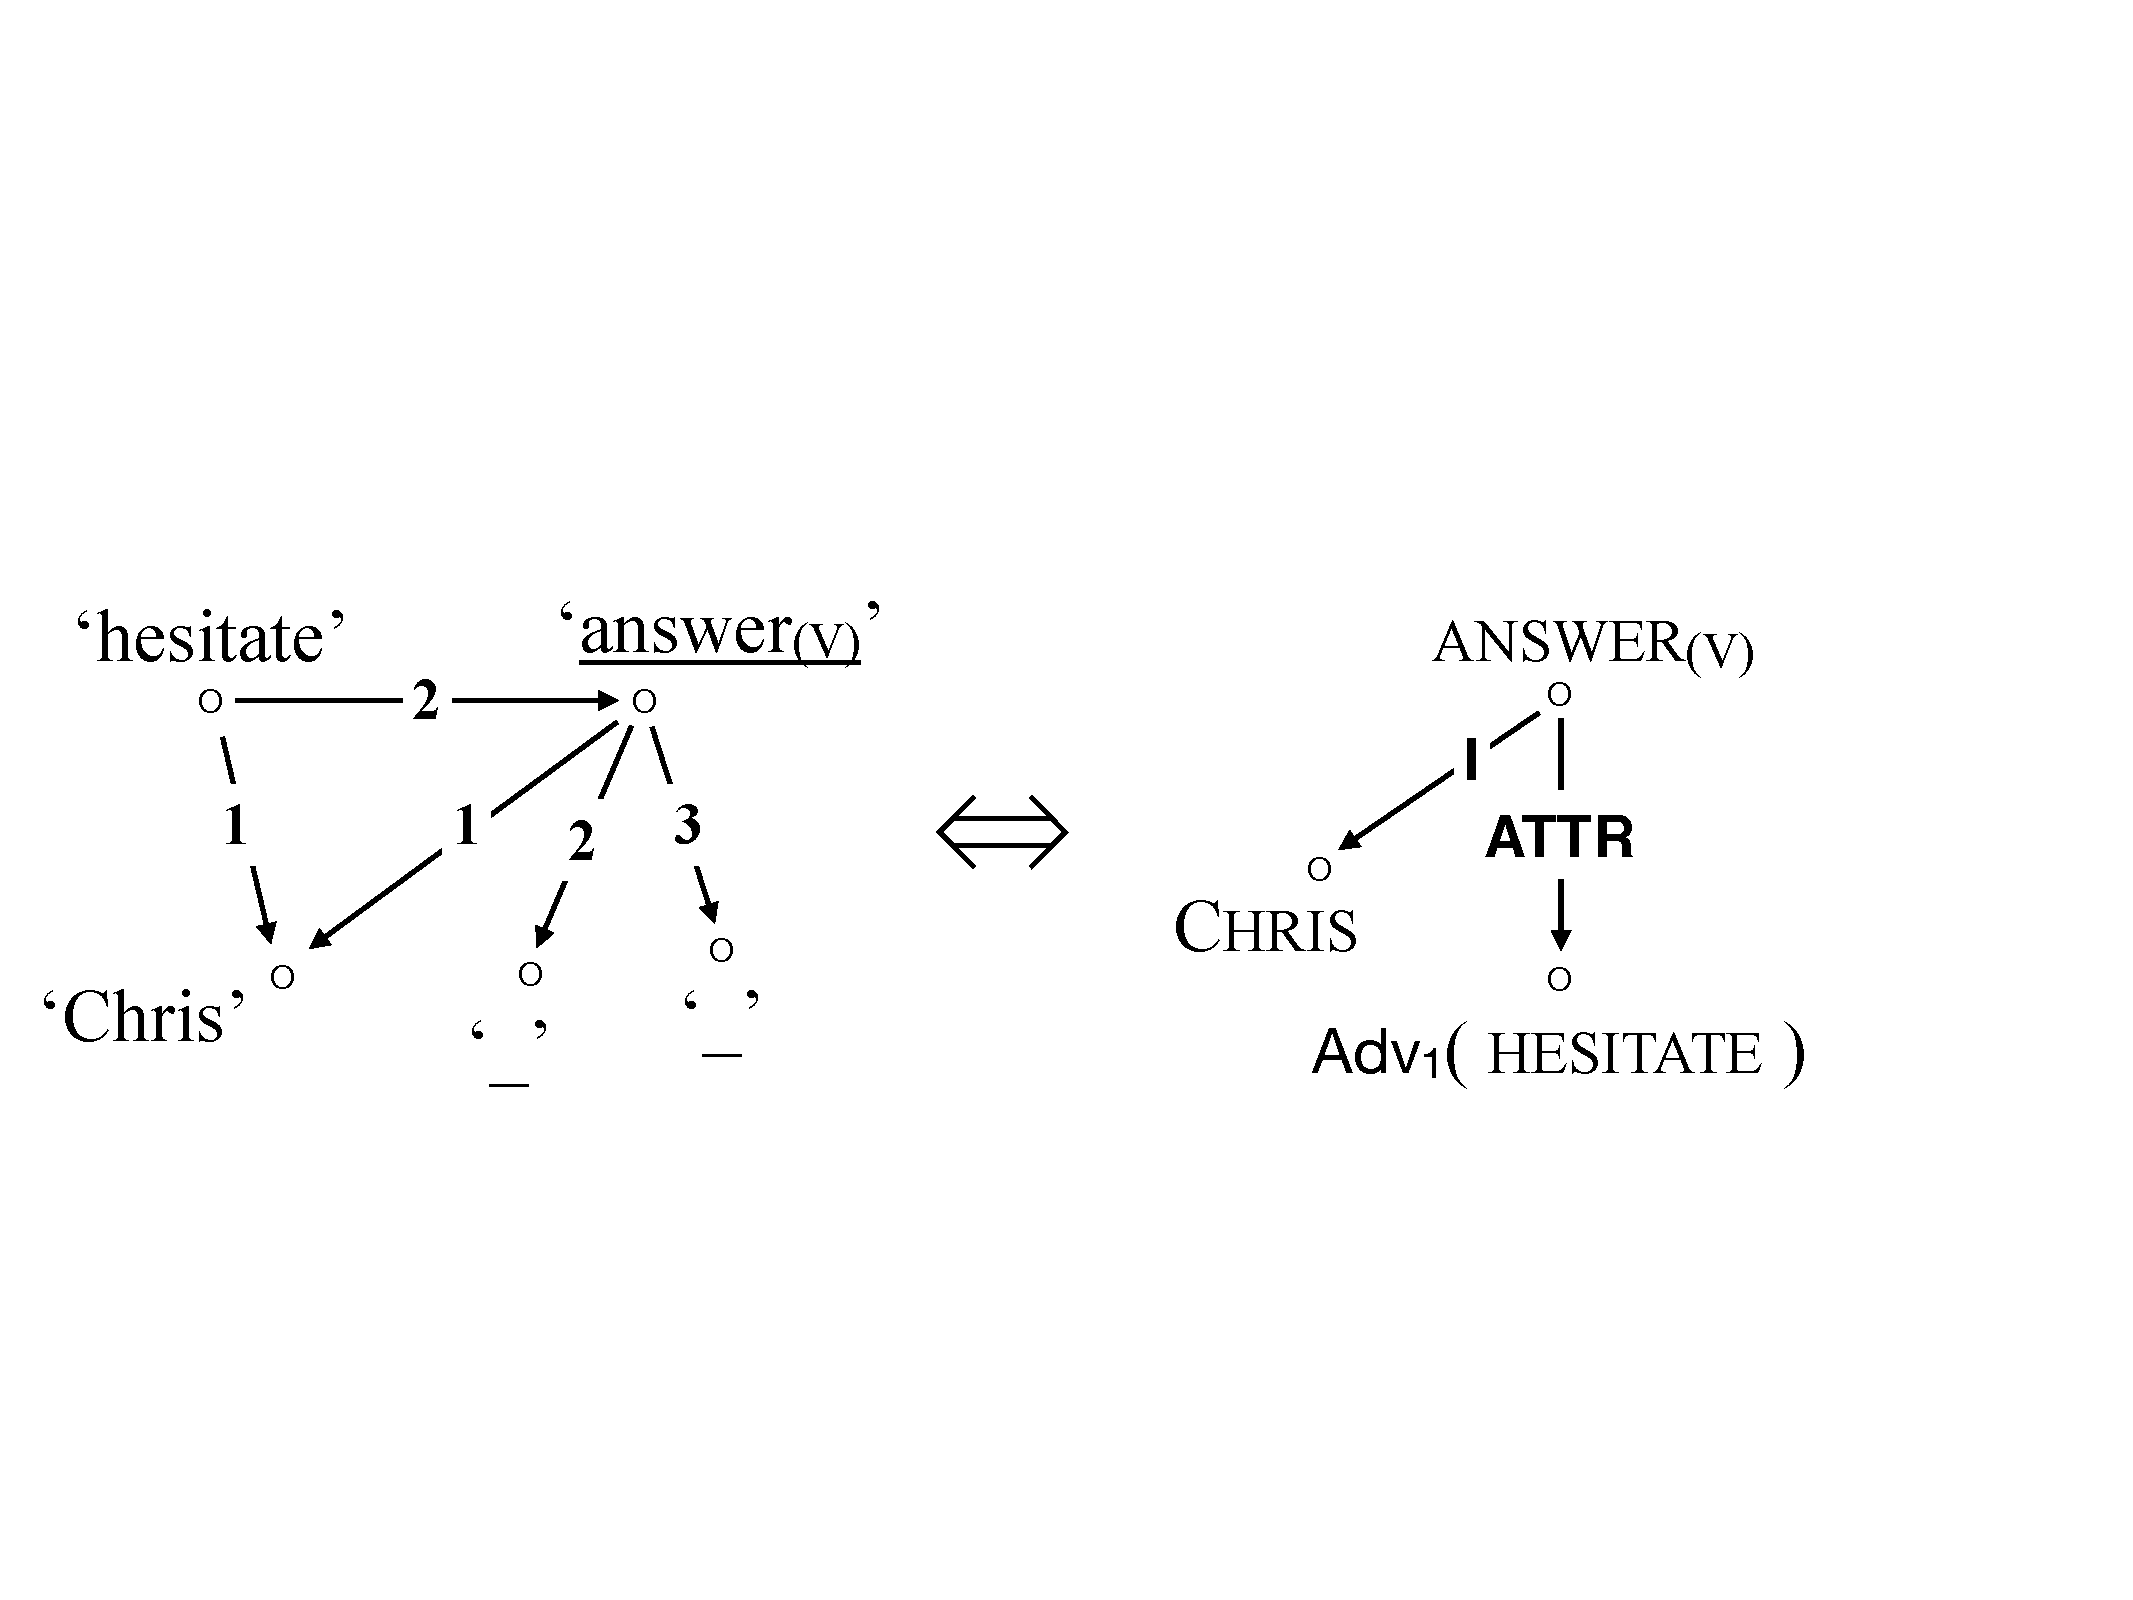
\includegraphics[width=9.5cm]{Fig/ParaLF/SemR-DSyntR-Adv1.pdf}
\caption{Sem\thinspace$\Leftrightarrow$\thinspace{}DSynt correspondence for the sentence \textit{Chris answers hesitatingly.}}\label{fig:Ch3-SemRDSyntR-Adv1}
\end{figure}

For \lfappl{Adv$_{2/3...}$}{L} things are more complicated since these adverbials involve a passive-like\index[notion]{voice, grammatical} use of L; for instance, see \Next, together with the corresponding Sem\thinspace$\Leftrightarrow$\thinspace{}DSynt correspondence in \figref{fig:Ch3-SemRDSyntR-Adv2}.

\begingroup
\small

\ex.\label{ex:ChapParaLF-ChrisFaintedUnderTheEyes} Chris fainted \emph{\idiom{under the eyes}}\tsub{\lfappl{Adv$_2$}{\textit{look}\tsub{(V)}}} of his uncle.

\endgroup

\begin{figure}

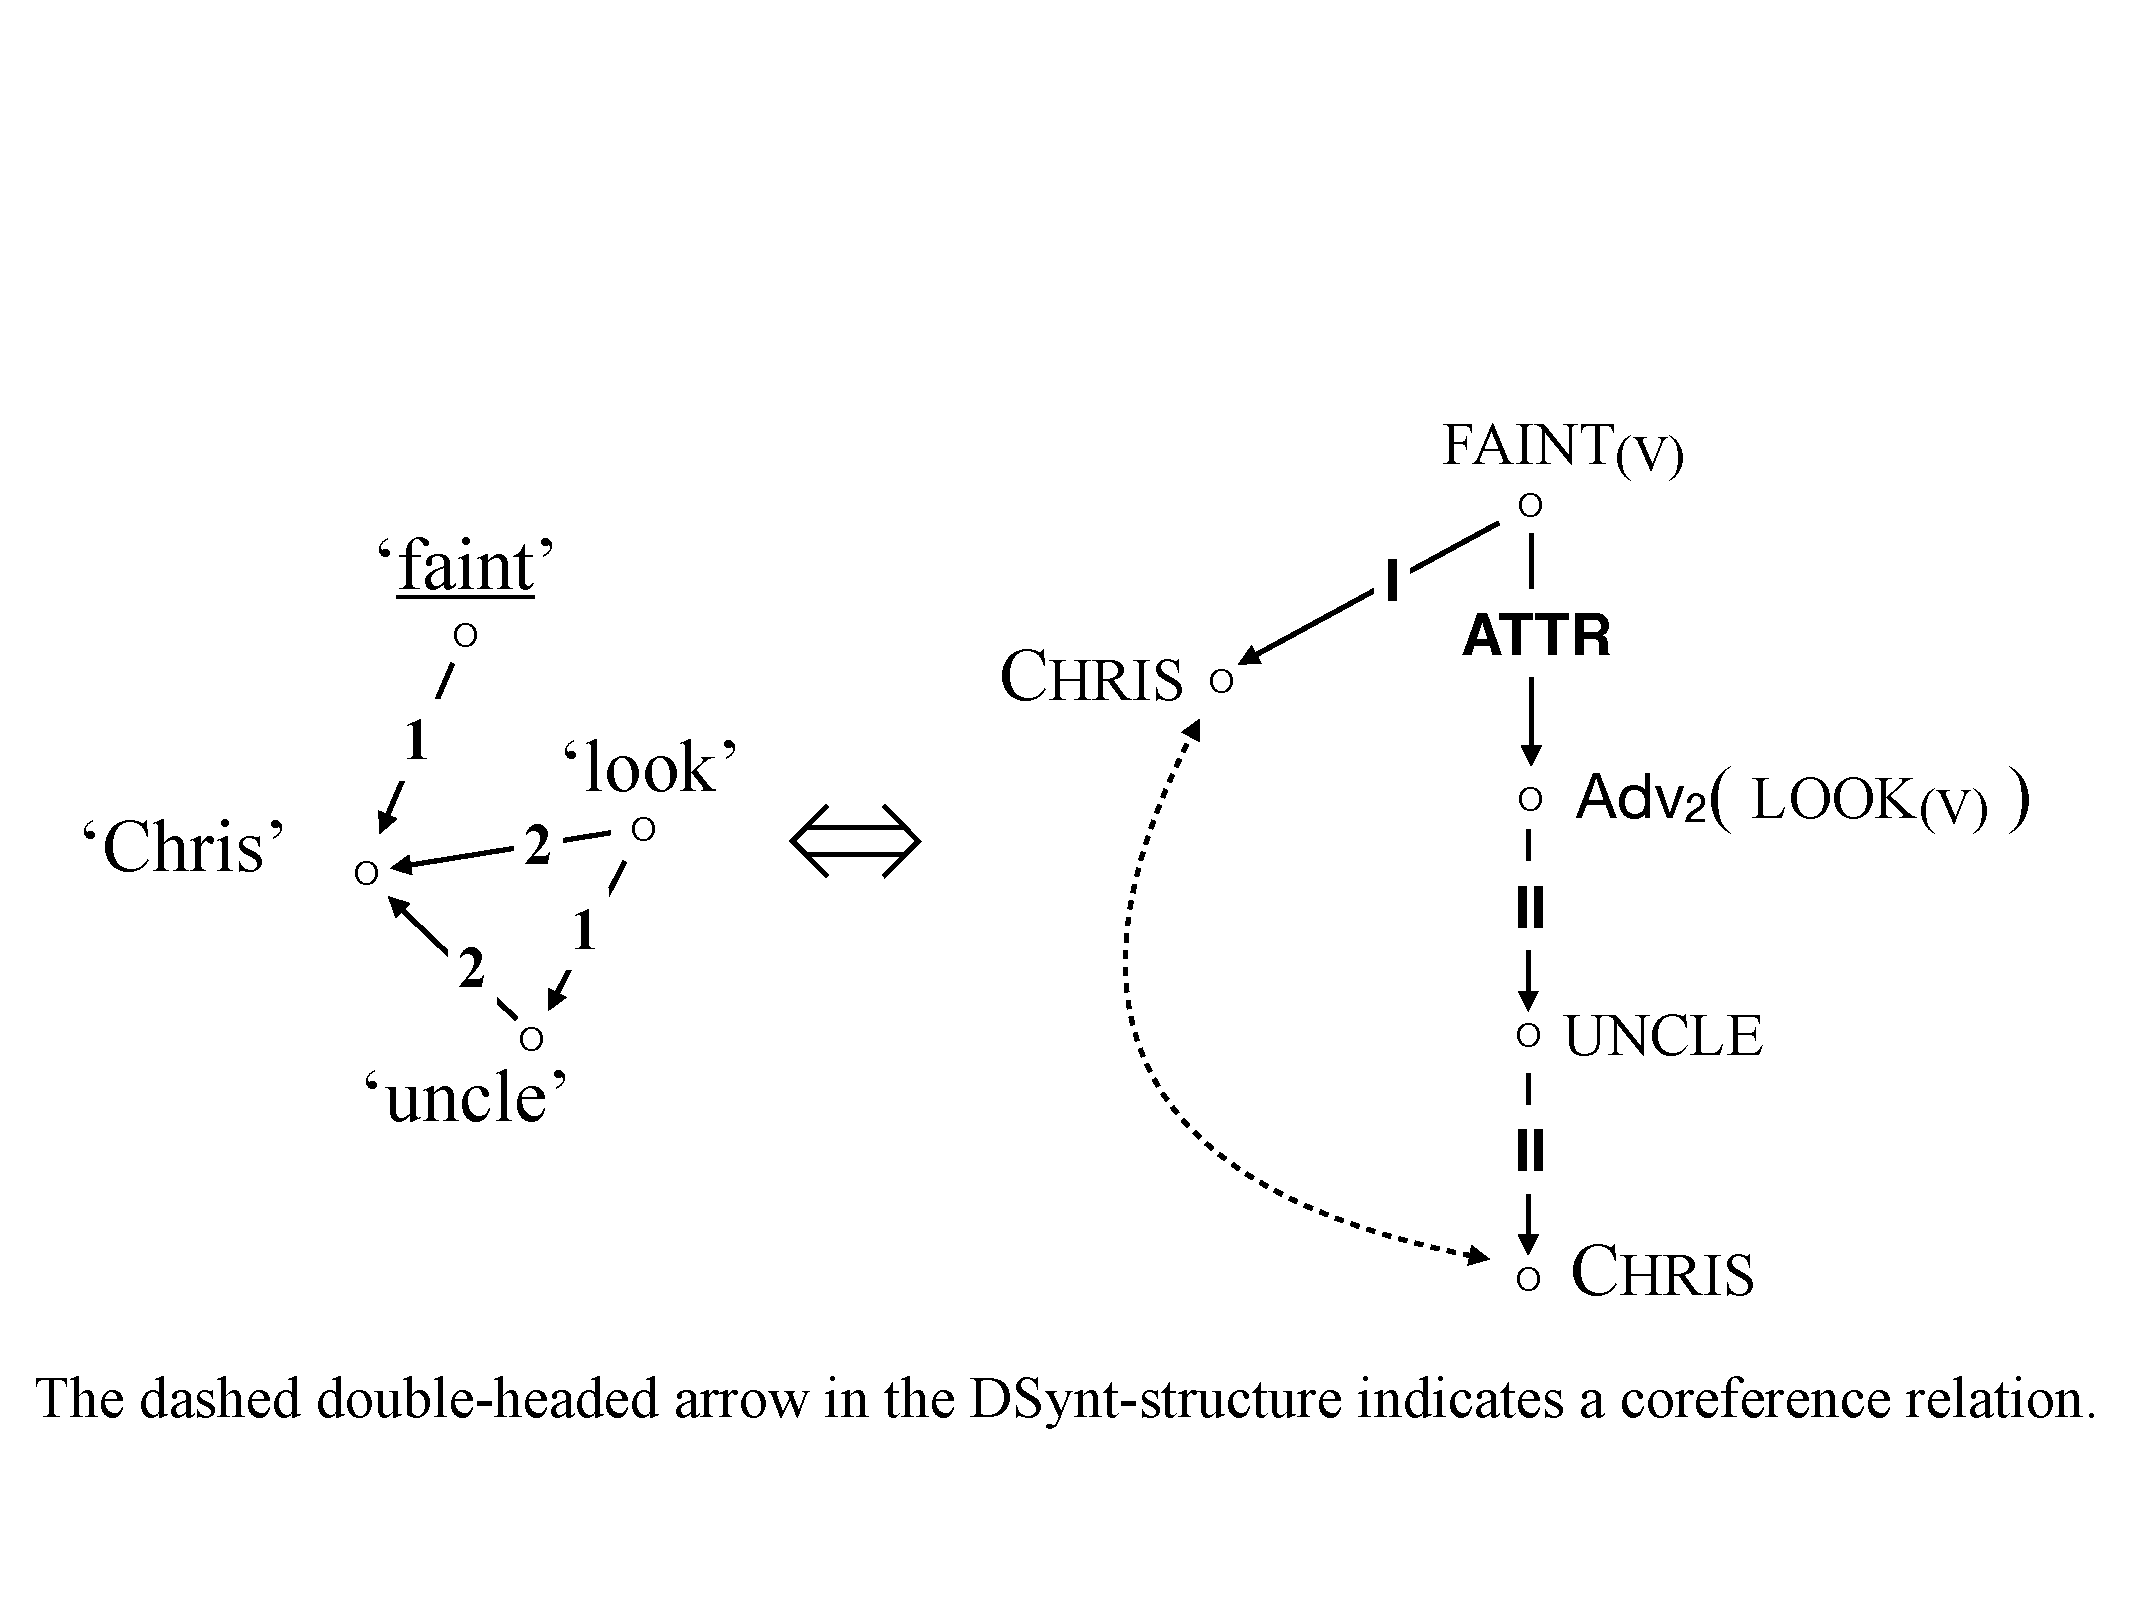
\includegraphics[width=9.5cm]{Fig/ParaLF/SemR-DSyntR-Adv2.pdf}
\caption{Sem\thinspace$\Leftrightarrow$\thinspace{}DSynt correspondence for the sentence \textit{Chris fainted under the eyes of his uncle.}}\label{fig:Ch3-SemRDSyntR-Adv2}
\end{figure}

In the DSynt-tree of \figref{fig:Ch3-SemRDSyntR-Adv2}, \textsc{uncle} appears as DSyntA\thinspace\syntDname{II} of \lfappl{Adv$_2$}{\textit{look}\tsub{(V)}} because this adverbial is equivalent to a passive form of \textsc{look}\tsub{(V)}: \idiom{\textit{under the eyes}} \textit{of his uncle}\enskip{\small $\equiv$}\enskip\textit{being looked at by his uncle}.

\paragraph*{Comment~2.}\label{para:comment2Advi}

A specific subset of lexical entities that are \lfappl{Adv\tsub{1}}{L} constitutes an exception to the statement in Comment~1: DSyntA\thinspace\syntDname{I} of these adverbials does not coincide with DSyntA\thinspace\syntDname{I} of the governing verb. Thus, in \Next, DSyntA\thinspace\syntDname{I} of \lf{Adv\tsub{1}} -- i.e. \textsc{Chris} -- does not coincide with DSyntA\thinspace\syntDname{I} of \textsc{vote}\tsub{(V)} -- i.e. \textsc{committee}:

\begingroup
\small

\ex. The committee voted \emph{in the absence} of Chris.

\endgroup

Other \lfappl{Adv\tsub{1}}{L} of the same type are \textit{in the presence} \lfgp{\textit{of} N\tsub{X}}, \textit{with the departure} \lfgp{\textit{of} N\tsub{X}}, \textit{with the illness}  \lfgp{\textit{of} N\tsub{X}}, etc.

All such adverbials are encoded by putting the \syntDname{1} actantial subscript\index[notion]{actantial subscript} between parentheses: \lfappl{Adv\tsub{(1)}}{L}\index[lf]{Advi@\lf{Adv\tsub{i}}!\lf{Adv\tsub{(i)}}|emph}. This notation indicates that the subscript does not do its normal job, but marks simultaneously two things:

\begin{itemize}

\item the non-coincidence between L's DSyntA\thinspace\syntDname{I} and that of the governing verb;

\item the obligatory character of the expression of L's DSyntA\thinspace\syntDname{I} with \lfappl{Adv\tsub{(1)}}{L}.

\end{itemize}

Consequently, the adverbial expression \textit{in the absence} in \Last is described by the LF formula \Next.

\begingroup
\small

\ex. \begingroup\setlength{\tabcolsep}{2pt}
\begin{tabular}[t]{ l l >{\raggedright\arraybackslash}p{6cm} }
\lfappl{Adv\tsub{(1)}}{\textit{absent}} & = & \textit{in the absence} \lfgp{\textit{of} N\tsub{X}} \\
\end{tabular}\endgroup

\endgroup

The \lf{Adv\tsub{1}} $\sim$ \lf{Adv\tsub{(1)}} contrast is parallel to the contrast between English regular V\tsub{\textsc{ing}} phrases with DSyntA\thinspace\syntDname{I} coinciding with DSyntA\thinspace\syntDname{I} of the governing verb \Next[a] and special V\tsub{\textsc{ing}} phrases whose DSyntA\thinspace\syntDname{I} does not \Next[b]:

\begingroup
\small

\ex. \a. \emph{Having left the house}, I heaved a sigh of relief.
     \b. \emph{My father having left the house}, I heaved a sigh of relief.

\endgroup

The V\tsub{\textsc{ing}} construction in \Last[b] is known as the \notion{absolute construction}\index[notion]{absolute construction}. Since \lf{Adv$_{(1)}$} lexical entities are, so to speak, the lexical embodiment of the absolute construction, it is convenient to call them \notion{absolutive adverbials}\index[notion]{adverb!absolutive \tld ial}.

\begin{historicalremark}
In several previous publications, \lf{Adv\tsub{i}} was erroneously classified as a syntagmatic LF -- see \textcite{Melcuk1982b}, \textcite{MelcukZholkovsky1984}, \textcite{Melcuketal1995-e} and \textcite{MelcukEtAl1999}.% The reason is that an element of an \lf{Adv\tsub{i}} is very often a preposition\index[notion]{preposition} governing a noun L, such as \textit{in silence} in the English illustrations on p.\thinspace\pageref{txt:Adv1IllustInSilence}.
\end{historicalremark}

\section{Singulative, collective and other inflection-like derivatives}\label{sec:flFlexion}

The LFs introduced in this section correspond to semantic derivatives manifesting a strong analogy with the expression of such inflectional\index[notion]{inflection} meanings as (noun) singular vs. plural, etc. These LFs come in two groups: (i)~those that have to do with quantity as regards L -- \lf{Sing} and \lf{Mult} -- and (ii) those that characterize the accomplishment of event L -- \lf{Imper}, \lf{Perf}, \lf{Imperf} and \lf{Result\tsub{i}}.

\refstepcounter{LFlist}
\subsubsection*{{\small [\arabic{LFlist}]} \lf{Sing} \lfgp{{\scriptsize Latin} \textit{singulus} `singular, unique'}: singulative}\label{lf:Sing}
\addcontentsline{toc}{subsection}{{\footnotesize [\arabic{LFlist}]} \lf{Sing}: singulative}\index[lf]{Sing@\lf{Sing}|emph}

\lfappl{Sing}{L} is a lexical entity that denotes a unit\slashs{}quantum of L's referent.

\begin{quote}
\begingroup
\small
\begin{tabular}{ l c c }
   \midrule
   \multicolumn{3}{l}{\lf{Sing}: verbal or nominal} \\
   \midrule
   \textbf{L} & V & N \\
   \midrule
   \textbf{\lfappl{Sing}{L}} & V & N \\
   \midrule
\end{tabular}
\endgroup
\end{quote}

\begin{longtable*}[l]{ l l >{\raggedright\arraybackslash}p{7cm} }

\multicolumn{3}{l}{\textbf{English}} \\*

\lfappl{S\tsub{0}Sing}{\textit{paint}\tsub{(V)}} & = & \idiom{\textit{brush stroke}} \\
\multicolumn{3}{ p{11cm} }{\leftskip=0.5cm{\small\remark{Note.}This is not a ``pure'' \lf{Sing} for a verb, but an \lf{S\tsub{0}Sing}, as it returns a nominal value. See the remark on verb singulatives after the illustrations.}} \\
\lfappl{Sing}{\textit{rice}} & = & \textit{grain of} \tld \\
\lfappl{Sing}{\textit{rain}\tsub{(N)}} & = & \textit{raindrop} \\
\lfappl{Sing}{\textit{parquet}} & = & \tld\ \textit{slat} \\
\lfappl{Sing}{\textit{body}} & = & \idiom{\textit{body part}} \\
\lfappl{Sing}{\textit{fur}\tsub{(N)}} & = & \textit{hair}\sensenum{3}\quad\lfgp{cf. \textit{hair}\sensenum{1} and \textit{hair}\sensenum{2} under \lf{Mult}, p.\thinspace\pageref{illustr:HAIR1-2}} \\
\lfappl{Sing}{\textit{vocabulary}} & = & \textit{word} \\[6pt]

\multicolumn{3}{l}{\textbf{French}} \\*

\lfappl{S\tsub{0}Sing}{\textit{peindre}} & = & \idiom{\textit{coup de pinceau}} \\
\lfappl{Sing}{\textit{riz}} & = & \textit{grain de} \tld \\
\lfappl{Sing}{\textit{pluie}} & = & \textit{goutte de} \tld \\
\lfappl{Sing}{\textit{parquet}} & = & \textit{lame de} \tld \\
\lfappl{Sing}{\textit{corps}} & = & \idiom{\textit{partie du corps}} \\
\lfappl{Sing}{\textit{pelage}} & = & \textit{poil} \\*
\lfappl{Sing}{\textit{vocabulaire}} & = & \textit{mot} \\[6pt]

\multicolumn{3}{l}{\textbf{Russian}} \\*

\lfappl{S\tsub{0}Sing}{\textit{pisat\palati} \lfgp{\textit{kartinu}}} & = & \textit{mazok} \\
\lfappl{Sing}{\textit{ris}} & = & \idiom{\textit{risovoe zërny\v{s}ko}}\textbf{,} \textit{risinka} \\
\lfappl{Sing}{\textit{do\v{z}d\suffixsplit\palati}} & = & \textit{kaplja} \tld\textit{ja} \\
\lfappl{Sing}{\textit{parket}} & = & \textit{parketina} \\
\lfappl{Sing}{\textit{telo}} & = & \idiom{\textit{\v{c}ast\palati\ tela}} \\
\lfappl{Sing}{\textit{mex}} & = & \textit{volos}\textbf{,} \textit{volosok} \\
\lfappl{Sing}{\textit{slovar\palati}} & = & \textit{slovo} \\

\end{longtable*}

In a \notion{Standard Average European} [SAE]\index[notion]{Standard Average European [SAE] language} language, the singulative typically applies to nouns, less frequently to verbs. Here are examples of verbal singulatives:

\begingroup
\small

\ex. \begingroup\setlength{\tabcolsep}{2pt}
\begin{tabular}[t]{ l l l >{\raggedright\arraybackslash}p{7cm} }
{\smaller English} & \lfappl{Sing}{\textit{beat}\tsub{(V)}} & = & \textit{hit}\tsub{(V)} \\
{\smaller French} & \lfappl{Sing}{\textit{battre}} & = & \textit{frapper} \\
{\smaller Russian} & \lfappl{Sing}{\textit{bit\palati}} & = & \textit{udarit\palati} \\
\end{tabular}\endgroup

\endgroup

Russian, with its inflectional category of aspect, has an important set of verbs whose perfective form expresses \lf{Sing}:

\begingroup
\small

\ex. \begingroup\setlength{\tabcolsep}{2pt}
\begin{tabular}[t]{ l l l l l }
\lfappl{Sing}{\textit{prygat\palati}} & `jump-\textsc{imperf}' & = & \textit{prygnut\palati} & `jump-\textsc{perf} = do one jump' \\
\lfappl{Sing}{\textit{udarjat\palati}} & `hit-\textsc{imperf}' & = & \textit{udarit\palati} & `hit-\textsc{perf} = give one blow' \\
\lfappl{Sing}{\textit{celovat\palati}} & `kiss-\textsc{imperf}' & = & \textit{pocelovat\palati} & `kiss-\textsc{perf} = give one kiss' \\
\end{tabular}\endgroup

\endgroup

\refstepcounter{LFlist}
\subsubsection*{{\small [\arabic{LFlist}]} \lf{Mult} \lfgp{{\scriptsize Latin} \textit{multum} `multitude'}: collective (for nouns)\slashs{}multiplicative (for verbs)}\label{lf:Mult}
\addcontentsline{toc}{subsection}{{\footnotesize [\arabic{LFlist}]} \lf{Mult}: collective (for nouns)\slashs{}multiplicative (for verbs)}\index[lf]{Mult@\lf{Mult}|emph}

\lfappl{Mult}{L} is a lexical entity that denotes a set of Ls forming a whole.

\begin{quote}
\begingroup

\begin{tabular}{ l c c }
   \midrule
   \multicolumn{3}{l}{\lf{Mult}: verbal or nominal} \\
   \midrule
   \textbf{L} & V & N \\
   \midrule
   \textbf{\lfappl{Mult}{L}} & V & N \\
   \midrule
\end{tabular}
\endgroup
\end{quote}

\phantomsection\label{illustr:HAIR1-2}\begin{longtable*}[l]{ l l >{\raggedright\arraybackslash}p{7cm} }

\multicolumn{3}{l}{\textbf{English}} \\*

\lfappl{Mult}{\textit{dog}} & = & \textit{pack}\tsub{(N)}\sensenum{II.1} \textit{of} \tld\textit{s} \\*
\lfappl{Mult}{\textit{lie}\tsub{(N)}} & = & \textit{pack}\tsub{(N)}\sensenum{II.4} \textit{of} \tld\textit{s} \\*
\lfappl{Mult}{\textit{hair}\sensenum{1}} & = & \textit{hair}\sensenum{2}\textbf{;} \idiom{\textit{head of hair}}\vspace{6pt} \\

\multicolumn{3}{l}{\textbf{French}} \\*

\lfappl{Mult}{\textit{chien}} & = & \textit{meute} \textit{de} \tld\textit{s} \\
\lfappl{Mult}{\textit{mensonge}} & = & \textit{tas} \textit{de} \tld\textit{s} \\
\lfappl{Mult}{\textit{cheveu}\sensenum{1}} & = & \textit{cheveux}\sensenum{2}\textbf{,} \textit{chevelure}\vspace{6pt} \\

\multicolumn{3}{l}{\textbf{Russian}} \\*

\lfappl{Mult}{\textit{sobak\suffixsplit{}a}} & = & \textit{svora} \tld \\
\lfappl{Mult}{\textit{l\suffixsplit{}o\v{z}\palati}} & = & \textit{ku\v{c}a} \tld\textit{\v{z}i} \\
\lfappl{Mult}{\textit{volos}\sensenum{1}} & = & \textit{volosy}\sensenum{2}\textbf{;} \textit{\v{s}eveljura} \\

\end{longtable*}

In parallel with singulative verbs, SAE languages\index[notion]{Standard Average European [SAE] language} show multiplicative verbs:\footnote{On the \lf{AntiMagn} LF used in \ref{ex:AntiMagn-Mult}, see \chapref{chap:syntLFs}, p.\thinspace\pageref{lf:AntiMagn}.}\index[lf]{AntiMagn@\lf{AntiMagn}}\index[lf]{Magn@\lf{Magn}!AntiMagn@\lf{AntiMagn}}

\begingroup
\small

\ex.\label{ex:AntiMagn-Mult} \begingroup\setlength{\tabcolsep}{2pt}
\begin{tabular}[t]{ l l l >{\raggedright\arraybackslash}p{6cm} }
{\smaller English} & \lfappl{AntiMagn+Mult}{\textit{jump}\tsub{(V)}} & = & \textit{hop}\tsub{(V)} \\
%French & \lfappl{AntiMagn\thinspace+\thinspace Mult}{\textit{sauter}} & = & \textit{sautiller} \\
{\smaller French} & \lfappl{AntiMagn+Mult}{\textit{taper}} & = & \textit{tapoter} \\
{\smaller Russian} & \lfappl{AntiMagn+Mult}{\textit{xlopat\palati}} & = & \textit{poxlopyvat\palati} \\
\end{tabular}\endgroup

\endgroup

\refstepcounter{LFlist}
\subsubsection*{{\small [\arabic{LFlist}]} \lf{Imper} \lfgp{{\scriptsize Latin} \textit{imper\={a}re} `[to] command, order'}: imperative}\label{lf:Imper}
\addcontentsline{toc}{subsection}{{\footnotesize [\arabic{LFlist}]} \lf{Imper}: imperative}\index[lf]{Imper@\lf{Imper}|emph}

\lfappl{Imper}{L} is an utterance by which the Speaker\index[notion]{Speaker, the} incites the Addressee\index[notion]{Addressee} to do L.

\begin{quote}
\begingroup
\small
\begin{tabular}{ l c }
   \midrule
   \multicolumn{2}{l}{\lf{Imper}: verbal or clausative\index[notion]{clausative}} \\
   \midrule
   \textbf{L} & V \\
   \midrule
   \textbf{\lfappl{Imper}{L}} & V\slashs{}Claus \\
   \midrule
\end{tabular}
\endgroup
\end{quote}

\begin{longtable*}[l]{ l l >{\raggedright\arraybackslash}p{6.5cm} }

\multicolumn{3}{l}{\textbf{English}} \\*

\lfappl{Imper}{\idiom{\textit{go away}}} & = & \uslabel{colloquial} \idiom{\textit{Beat it!}} \\
\lfappl{ImperPred}{\textit{quiet}\tsub{(Adj)}} & = & \textit{Quiet!}\textbf{,} \textit{Shush!}\textbf{,} \textit{Shh!} \\
\lfappl{Imper}{\idiom{\textit{give up}}} & = & \idiom{\textit{Let it go!}} \\
\lfappl{Imper}{\textit{Bang!}} & = & \textit{Fire!} \\
\lfappl{ImperPrepar\tsub{1}Real\tsub{1}}{\textit{meal}} & = & \textit{Breakfast} $\langle$\textit{Lunch} $\rangle$ $\langle$\textit{Supper}$\rangle$ \textit{is ready!} \\[6pt]

\multicolumn{3}{l}{\textbf{French}} \\*

\lfappl{Imper}{\textit{partir}} & = & \uslabel{offensive} \textit{Dégage !}\textbf{;} \uslabel{colloquial} \textit{Zou !} \\
\lfappl{Imper}{\textit{se taire}} & = & \textit{Chut !}\textbf{;} \uslabel{offensive} \idiom{\textit{Ta gueule !}} \\
\lfappl{Imper}{\idiom{\textit{tenir le coup}}} & = & \textit{Courage !} \\
\lfappl{Imper}{\textit{venir}} & = & \textit{Ici !} \\
\lfappl{Imper\tsub{$\supset$}}{\idiom{\textit{laisser le passage}}} & = & \idiom{\textit{Chaud devant !}} \\
\lfappl{Imper}{\textit{Pan !}} & = & \textit{Feu !} \\
\lfappl{Imper}{\textit{abandonner}} & = & \idiom{\textit{Laisse tomber !}} \\*
\lfappl{ImperPrepar\tsub{1}Real\tsub{1}}{\textit{repas}} & = & \textit{À table !} \\[6pt]

\multicolumn{3}{l}{\textbf{Russian}} \\*

\lfappl{Imper}{\textit{ujti}} & = & \uslabel{offensive} \textit{Von} (\textit{otsjuda})\textit{!}\textbf{,} \uslabel{colloquial offensive} \textit{Po\v{s}ël von} (\textit{otsjuda})\textit{!} \\
\lfappl{Imper}{\textit{ne \v{s}umet\palati}} & = & \textit{Tixo!}\textbf{,} \textit{Tss!}\textbf{,} \textit{T\v{s}\v{s}!} \\
\lfappl{Imper}{\textit{vzjat\palati}} & = & \textit{Na}(\textit{te})\textit{!} \\*
\lfappl{Imper}{\uslabel{child language} \textit{Pif-paf!}} & = & \textit{Ogon\palati!} \\
\lfappl{ImperPrepar\tsub{1}Real\tsub{1}}{\textit{eda}} & = & (\textit{Pro\v{s}u vsex}) \textit{za stol!}\textbf{,} (\textit{Pro\v{s}u vsex}) \textit{k stolu!} \\

\end{longtable*}

\refstepcounter{LFlist}
\subsubsection*{{\small [\arabic{LFlist}]} \lf{Perf} \lfgp{{\scriptsize Latin} \textit{perfectum}}: perfective}\label{lf:Perf}
\addcontentsline{toc}{subsection}{{\footnotesize [\arabic{LFlist}]} \lf{Perf}: perfective}\index[lf]{Perf@\lf{Perf}|emph}

\lfappl{Perf}{L} is a verbal or clausative\index[notion]{clausative} lexical unit that denotes the fact of reaching the goal\verythinspace/\verythinspace{}limit inherent to the meaning of L -- cf. the comment that follows the illustrations for the LF \lf{Result\tsub{i}} below ([\ref{lf:Result-i}], p.\thinspace\pageref{txt:ResultvsPerf}).

\lf{Perf} and the following LF \lf{Imperf}\index[lf]{Imperf@\lf{Imperf}} correspond to aspectual meanings grammaticalized in Slavic languages, where they are inflectional\index[notion]{inflection}.

\begin{quote}
\begingroup
\small
\begin{tabular}{ l c }
   \midrule
   \multicolumn{2}{l}{\lf{Perf}: verbal or clausative} \\
   \midrule
   \textbf{L} & V \\
   \midrule
   \textbf{\lfappl{Perf}{L}} & V\slashs{}Claus \\
   \midrule
\end{tabular}
\endgroup
\end{quote}

\begin{longtable*}[l]{ l l >{\raggedright\arraybackslash}p{6cm} }

\multicolumn{3}{l}{\textbf{English}} \\*

\lfappl{Perf}{\textit{end}\tsub{(V)}} & = & \idiom{\textit{be over}} \\
\lfappl{Perf}{\textit{undress}} & = & \textit{have undressed} \\
\lfappl{Claus\tsub{0}Perf}{\textit{dive}\tsub{(V)}}\index[lf]{Claus0Perf@\lf{Claus\tsub{0}Perf}} & = & \textit{Splash!} \\[6pt]

\multicolumn{3}{l}{\textbf{French}} \\*

\lfappl{Perf}{\textit{revenir}} & = & \idiom{\textit{être de retour}} \\
\lfappl{Perf}{\textit{se déshabiller}} & = & \textit{s'être déshabillé} \\
\lfappl{Claus\tsub{0}Perf}{\textit{plonger}} & = & \textit{Plouf !} \\[6pt]

\multicolumn{3}{l}{\textbf{Russian}} \\*

\lfappl{Perf}{\textit{razdevat\palati{}sja}}  & = & \textit{razdet\palati{}sja} \\
\lfappl{Perf}{\textit{odevat\palati{}sja}}  & = & \textit{odet\palati{}sja} \\
\lfappl{Claus\tsub{0}Perf}{\textit{padat\palati} \lfgp{in a liquid}}  & = & \textit{Bux!}\textbf{,} \textit{Pljux!} \\

\end{longtable*}

Values of \lfappl{Perf}{L} and \lfappl{Imperf}{L} are mostly trivial, in the sense that they are usually grammatical forms of a verb L. \lf{Perf} is mainly used in complex LF formulas such as \lf{S\tsub{i}Perf}\phantomsection\label{lf:S-iPerf}\index[lf]{Si@\lf{S\tsub{i}}}, \lf{A\tsub{i}Perf}\phantomsection\label{lf:A-iPerf}\index[lf]{Ai@\lf{A\tsub{i}}} or \lf{PerfOper\tsub{i}}\phantomsection\label{lf:PerfOper-i}\index[lf]{Operi@\lf{Oper\tsub{i}}}.

\begingroup
\small

\ex. \begingroup\setlength{\tabcolsep}{2pt}
\begin{tabular}[t]{ l l >{\raggedright\arraybackslash}p{7cm} }
\lfappl{S\tsub{1}Perf}{\idiom{\textit{give birth}}} & = & \idiom{\textit{new mother}} \\
\lfappl{A\tsub{2}Perf}{\textit{cook}\tsub{(V)}} & = & \textit{cooked} \\
\lfappl{PerfOper{\tsub{1}}}{\textit{divorce}\tsub{(N)}} & = & \textit{get} \lfgp{\textsc{art} \tld} \\
\end{tabular}\endgroup

\endgroup

\refstepcounter{LFlist}
\subsubsection*{{\small [\arabic{LFlist}]} \lf{Imperf} \lfgp{{\scriptsize Latin} \textit{imperfectum}}: imperfective}\label{lf:Imperf}
\addcontentsline{toc}{subsection}{{\footnotesize [\arabic{LFlist}]} \lf{Imperf}: imperfective}\index[lf]{Imperf@\lf{Imperf}|emph}

\lfappl{Imperf}{L} is a verbal or clausative\index[notion]{clausative} lexical unit that denotes fact L as ongoing process and, eventually (as in Slavic languages), as the iteration of fact L.

\begin{quote}
\begingroup
\small
\begin{tabular}{ l c }
   \midrule
   \multicolumn{2}{l}{\lf{Imperf}: verbal or clausative} \\
   \midrule
   \textbf{L} & V \\
   \midrule
   \textbf{\lfappl{Imperf}{L}} & V\slashs{}Claus \\
   \midrule
\end{tabular}
\endgroup
\end{quote}

\begin{longtable*}[l]{ l l >{\raggedright\arraybackslash}p{6cm} }

\multicolumn{3}{l}{\textbf{English}} \\*

\lfappl{Imperf}{\idiom{\textit{be over}}} & = & \textit{end}\tsub{(V)}\textbf{,} \textit{finish}\tsub{(V)}\vspace{6pt} \\

\multicolumn{3}{l}{\textbf{French}} \\*

\lfappl{Imperf}{\textit{se réveiller}} & = & \uslabel{colloquial} \textit{émerger}\vspace{6pt} \\

\multicolumn{3}{l}{\textbf{Russian}} \\*

\lfappl{Imperf}{\textit{vernut\palati{}sja}}  & = & \textit{vozvra\v{s}\v{c}at\palati{}sja} \\
\lfappl{Imperf}{\textit{odet\palati{}sja}}  & = & \textit{odevat\palati{}sja} \\

\end{longtable*}

\refstepcounter{LFlist}
\subsubsection*{{\small [\arabic{LFlist}]} \lf{Result\tsub{i}} \lfgp{{\scriptsize Latin} *\textit{result\={a}re} `[to] result'}: resultative}\label{lf:Result-i}
\addcontentsline{toc}{subsection}{{\footnotesize [\arabic{LFlist}]} \lf{Result\tsub{i}}: resultative}\index[lf]{Resulti@\lf{Result\tsub{i}}|emph}

\lfappl{Result\tsub{i}}{L} is a verbal or clausative\index[notion]{clausative} lexical unit that denotes a situation \emph{necessarily} resulting from reaching the goal\slashs{}limit inherent to the meaning of L. DSyntA\thinspace\syntDname{I} of \lfappl{Result\tsub{i}}{L} corresponds to DSyntA\thinspace\syntDname{i} of L.

Let it be emphasized that the situation denoted by \lfappl{Result\tsub{i}}{L} is the necessary result of reaching L's goal\slashs{}limit. This is in contrast with some cases of \lfappl{Real\tsub{i}}{L}\index[lf]{Reali@\lf{Real\tsub{i}}} that are considered in \chapref{chap:syntLFs} (\sectref{sec:verbeReal}, [\ref{lf:Real-i}], ``\nameref*{par:RealVFusion},'' p.\thinspace\pageref{par:RealVFusion}), where the situation referred to by \lfappl{\lf{Real\tsub{i}}}{L} can be achieved in different ways.

\begin{quote}
\begingroup
\small
\begin{tabular}{ l c }
   \midrule
   \multicolumn{2}{l}{\lf{Result\tsub{i}}: verbal or clausative} \\
   \midrule
   \textbf{L} & V  \\
   \midrule
   \textbf{\lfappl{Result\tsub{i}}{L}} & V\slashs{}Claus \\
   \midrule
\end{tabular}
\endgroup
\end{quote}

\begin{longtable*}[l]{ l l >{\raggedright\arraybackslash}p{5cm} }

\multicolumn{3}{l}{\textbf{English}} \\*

\lfappl{Result\tsub{1}}{\textit{reach}\tsub{(V)} \lfgp{N\tsub{Y}}} & = & \textit{be} \lfgp{\lf{Loc\tsub{in}} N\tsub{Y}} \\[1pt]
\multicolumn{3}{ p{11cm} }{\leftskip=0.5cm{\small\remark{Note.}For the syntagmatic LF \lf{Loc\tsub{in}} (locative preposition meaning `being located in'), see \chapref{chap:syntLFs}, [\ref{lf:Loc-in}], p.\thinspace\pageref{lf:Loc-in}.}}\index[lf]{Locin@\lf{Loc\tsub{in}}} \\[1pt]
\lfappl{Result\tsub{1}}{\uslabel{colloquial} \idiom{\textit{drift off}}} & = & \textit{sleep}\tsub{(V)}\textbf{;} \textit{Zzz!} \\
\lfappl{Result\tsub{1}}{\textit{agonize}} & = & \textit{die}\tsub{(V)} \\
\lfappl{Result\tsub{1}}{\textit{die}\tsub{(V)}} & = & \uslabel{colloquial} \idiom{\textit{push up daisies}} \\
\lfappl{Result\tsub{1}}{\textit{acquire}} & = & \textit{own}\tsub{(V)} \\*
\lfappl{Result\tsub{2}}{\uslabel{colloquial} \idiom{\textit{shut up}}\sensenum{2} \lfgp{N\tsub{Y}}} & = & \uslabel{colloquial} \lfgp{N\tsub{Y}} \idiom{\textit{shut up}}\sensenum{1} \\[6pt]

\multicolumn{3}{l}{\textbf{French}} \\*

%%%\lfappl{Result\tsub{1}}{\textit{s'approcher} \lfgp{\textit{de} N\tsub{Y}}} & = & \textit{atteindre} \lfgp{N\tsub{Y}} \\ @@@ Real1 ?
\lfappl{Result\tsub{1}}{\textit{atteindre} \lfgp{N\tsub{Y}}} & = & \textit{être} \lfgp{\lf{Loc\tsub{in}} N\tsub{Y}} \\
\lfappl{Result\tsub{1}}{\textit{s'endormir}} & = & \textit{dormir}\textbf{;} \textit{Zzz~!} \\
\lfappl{Result\tsub{1}}{\textit{agoniser}} & = & \textit{mourir} \\
\lfappl{Result\tsub{1}}{\textit{mourir}} & = & \uslabel{colloquial} $\ulcorner$\textit{manger les pissenlits par la racine}$\urcorner$ \\
\lfappl{Result\tsub{1}}{\textit{acquérir}} & = & \textit{posséder} \\
\lfappl{Result\tsub{2}}{\uslabel{colloquial} \idiom{\textit{clouer le bec}} \lfgp{\textit{à} N\tsub{Y}}} & = & \lfgp{N\tsub{Y}} \textit{se taire} \\[6pt]
%\lfappl{\lf{S\tsub{0}}Result\tsub{1}}{\textit{se souler}} & = & \idiom{\textit{gueule de bois}} \\ Intéressant, mais ce n'est pas une situation résultant NÉCESSAIREMENT du fait de se saouler.

\multicolumn{3}{l}{\textbf{Russian}} \\*

\lfappl{Result\tsub{1}}{\textit{dosti\v{c}\palati} \lfgp{N\tsub{Y-\textsc{gen}}}} & = & \textit{byt\palati} \lfgp{\lf{Loc\tsub{in}} N\tsub{Y}} \\
\lfappl{Result\tsub{1}}{\textit{zasnut\palati}} & = & \textit{spat\palati}\textbf{;} \textit{Xrrr...!} \\
\lfappl{Result\tsub{1}}{\textit{agonizirovat\palati}} & = & \textit{umeret\palati} \\
\lfappl{Result\tsub{1}}{\textit{umeret\palati}} & = & \uslabel{colloquial} \idiom{\textit{byt\palati na tom svete}} \\
\lfappl{Result\tsub{1}}{\textit{priobresti}} & = & \textit{vladet\palati} \\
\lfappl{Result\tsub{2}}{\uslabel{colloquial} \idiom{\textit{zatknut\palati\ rot}} \lfgp{N\tsub{Y-\textsc{dat}}}} & = & \lfgp{N\tsub{Y-\textsc{nom}}} \textit{zamol\v{c}at\palati}\textbf{,} \uslabel{colloquial} \textit{zatknut\palati{}sja}\textbf{;} \textit{Ni\onewdf{}gugu}\tsub{(Interj)} \\

\end{longtable*}

\phantomsection\label{txt:ResultvsPerf}\lf{Result\tsub{i}} must be distinguished from \lf{Perf}\index[lf]{Perf@\lf{Perf}}, for which it could be mistaken. For instance, \Next[a] has a different meaning from \Next[b]:

\begingroup
\small

\ex. \a. \textit{have reached}\tsub{\lfappl{Perf}{\textit{reach}\tsub{(V)}}} \textit{Montreal}
     \b. \textit{be}\tsub{\lfappl{Result\tsub{1}}{\textit{reach}\tsub{(V)}}} \textit{in Montreal}

\endgroup

\lfappl{Perf}{L} denotes the same fact as L but in a different state: `have reached' is still `reach', but `completed'. On the contrary, \lfappl{Result\tsub{i}}{L} denotes a different fact: the situation which is necessarily entailed by reaching L's goal\verythinspace/\verythinspace{}limit and in which L's DSyntA\thinspace\syntDname{i} finds itself. 

\clearpage{\pagestyle{empty}\cleardoublepage}

